\documentclass[12pt,chapterheads,oneside]{ucsd}

\usepackage{amsmath, amscd, amssymb, amsthm}
\usepackage{graphicx}
\usepackage{xfrac}
\usepackage{color}
\usepackage{multirow}
\usepackage{multicol}
\usepackage{ifthen}
\usepackage{xspace}
\usepackage{calc}
\usepackage{diagbox}
\usepackage{subfig}
\usepackage[T1]{fontenc}
\usepackage{mathptmx}
\usepackage{makeidx}
\usepackage[bottom]{footmisc}
\usepackage[hyphens]{url}
\usepackage[color=red!40,textwidth=24mm,textsize=footnotesize]{todonotes}
\usepackage[hidelinks,linktocpage,breaklinks]{hyperref}                                  
\usepackage{rotating}
\usepackage{afterpage}
\usepackage{xparse}
\usepackage{lineno}
\usepackage{slashed}
\usepackage{bm}
\usepackage{caption}
\usepackage{ragged2e}
%\usepackage{setspace} 
\usepackage{lmodern}% http://ctan.org/pkg/lm
%% \usepackage[style=base]{caption}
%% \captionsetup{style=base}
\usepackage{url}

\hypersetup{ pdfauthor   = {Doe, John},
             pdftitle    = {The Title},
             pdfkeywords = {},
             pdfcreator  = {LaTeX with hyperref package},
             pdfproducer = {LaTeX} }

%%%%%%%%%%%%%%%%%%%%%%%%%%%%%%%%%%%%%%%%%%%%%%%%%%%%%%%%%%%%%%%%%%%%
%
%  CMS Common definitions style file
%
%  N.B. use of \newcommand rather than \newcommand means
%       that a definition is ignored if already specified
%
%                                              L. Taylor 18 Feb 2005
%%%%%%%%%%%%%%%%%%%%%%%%%%%%%%%%%%%%%%%%%%%%%%%%%%%%%%%%%%%%%%%%%%%%

% Some shorthand
% turn off italics
\newcommand {\etal}{\mbox{et al.}\xspace} %et al. - no preceding comma
\newcommand {\ie}{\mbox{i.e.}\xspace}     %i.e.
\newcommand {\eg}{\mbox{e.g.}\xspace}     %e.g.
\newcommand {\etc}{\mbox{etc.}\xspace}     %etc.
\newcommand {\vs}{\mbox{\sl vs.}\xspace}      %vs.
\newcommand {\mdash}{\ensuremath{\mathrm{-}}} % for use within formulas

% some terms whose definition we may change
\newcommand {\Lone}{Level-1\xspace} % Level-1 or L1 ?
\newcommand {\Ltwo}{Level-2\xspace}
\newcommand {\Lthree}{Level-3\xspace}

% Some software programs (alphabetized)
\newcommand{\ACERMC} {\textsc{AcerMC}\xspace}
\newcommand{\ALPGEN} {{\textsc{alpgen}}\xspace}
\newcommand{\CHARYBDIS} {{\textsc{charybdis}}\xspace}
\newcommand{\CMKIN} {\textsc{cmkin}\xspace}
\newcommand{\CMSIM} {{\textsc{cmsim}}\xspace}
\newcommand{\CMSSW} {{\textsc{cmssw}}\xspace}
\newcommand{\COBRA} {{\textsc{cobra}}\xspace}
\newcommand{\COCOA} {{\textsc{cocoa}}\xspace}
\newcommand{\COMPHEP} {\textsc{CompHEP}\xspace}
\newcommand{\CTTEN} {\textsc{cteq10}\xspace}
\newcommand{\EVTGEN} {{\textsc{evtgen}}\xspace}
\newcommand{\FAMOS} {{\textsc{famos}}\xspace}
\newcommand{\GARCON} {\textsc{garcon}\xspace}
\newcommand{\GARFIELD} {{\textsc{garfield}}\xspace}
\newcommand{\GEANE} {{\textsc{geane}}\xspace}
\newcommand{\GEANTfour} {{\textsc{geant4}}\xspace}
\newcommand{\GEANTthree} {{\textsc{geant3}}\xspace}
\newcommand{\GEANT} {{\textsc{geant}}\xspace}
\newcommand{\HDECAY} {\textsc{hdecay}\xspace}
\newcommand{\HERWIG} {{\textsc{herwig}}\xspace}
\newcommand{\HIGLU} {{\textsc{higlu}}\xspace}
\newcommand{\HIJING} {{\textsc{hijing}}\xspace}
\newcommand{\IGUANA} {\textsc{iguana}\xspace}
\newcommand{\ISAJET} {{\textsc{isajet}}\xspace}
\newcommand{\ISAPYTHIA} {{\textsc{isapythia}}\xspace}
\newcommand{\ISASUGRA} {{\textsc{isasugra}}\xspace}
\newcommand{\ISASUSY} {{\textsc{isasusy}}\xspace}
\newcommand{\ISAWIG} {{\textsc{isawig}}\xspace}
\newcommand{\JIMMY} {{\textsc{jimmy}}\xspace}
\newcommand{\MADGRAPH} {\textsc{MadGraph}\xspace}
\newcommand{\MSTW} {\textsc{mstw2008}\xspace}
\newcommand{\NNPDF} {\textsc{nnpdf}\xspace}
\newcommand{\GGTWW}  {{\textsc{gg2ww}}\xspace}
\newcommand{\POWHEG} {\textsc{powheg}\xspace}
\newcommand{\HqT} {\textsc{HqT}\xspace}
\newcommand{\MCATNLO} {\textsc{mc@nlo}\xspace}
\newcommand{\MCFM} {\textsc{mcfm}\xspace}
\newcommand{\FEWZ} {\textsc{fewz}\xspace}
\newcommand{\MILLEPEDE} {{\textsc{millepede}}\xspace}
\newcommand{\ORCA} {{\textsc{orca}}\xspace}
\newcommand{\OSCAR} {{\textsc{oscar}}\xspace}
\newcommand{\PHOTOS} {\textsc{photos}\xspace}
\newcommand{\PROSPINO} {\textsc{prospino}\xspace}
\newcommand{\PYTHIA} {{\textsc{pythia}}\xspace}
\newcommand{\SHERPA} {{\textsc{sherpa}}\xspace}
\newcommand{\TAUOLA} {\textsc{tauola}\xspace}
\newcommand{\TOPREX} {\textsc{TopReX}\xspace}
\newcommand{\XDAQ} {{\textsc{xdaq}}\xspace}


%  Experiments
\newcommand {\DZERO}{D0\xspace}     %etc.


% Measurements and units...

\newcommand{\de}{\ensuremath{^\circ}}
\newcommand{\ten}[1]{\ensuremath{\times \text{10}^\text{#1}}}
\newcommand{\unit}[1]{\ensuremath{\text{\,#1}}\xspace}
\newcommand{\mum}{\ensuremath{\,\mu\text{m}}\xspace}
\newcommand{\micron}{\ensuremath{\,\mu\text{m}}\xspace}
\newcommand{\cm}{\ensuremath{\,\text{cm}}\xspace}
\newcommand{\cmcm}{\ensuremath{\,\text{cm^2}}\xspace}
\newcommand{\s}{\ensuremath{\,\text{s}}\xspace}
\newcommand{\ns}{\ensuremath{\,\text{ns}}\xspace}
% \newcommand{\mm}{\ensuremath{\,\text{mm}}\xspace}
\newcommand{\mus}{\ensuremath{\,\mu\text{s}}\xspace}
\newcommand{\keV}{\ensuremath{\,\text{ke\hspace{-.08em}V}}\xspace}
\newcommand{\MeV}{\ensuremath{\,\text{Me\hspace{-.08em}V}}\xspace}
\newcommand{\GeV}{\ensuremath{\,\text{Ge\hspace{-.08em}V}}\xspace}
\newcommand{\gev}{\GeV}
\newcommand{\TeV}{\ensuremath{\,\text{Te\hspace{-.08em}V}}\xspace}
\newcommand{\PeV}{\ensuremath{\,\text{Pe\hspace{-.08em}V}}\xspace}
\newcommand{\keVc}{\ensuremath{{\,\text{ke\hspace{-.08em}V\hspace{-0.16em}/\hspace{-0.08em}}c}}\xspace}
\newcommand{\MeVc}{\ensuremath{{\,\text{Me\hspace{-.08em}V\hspace{-0.16em}/\hspace{-0.08em}}c}}\xspace}
\newcommand{\GeVc}{\ensuremath{{\,\text{Ge\hspace{-.08em}V\hspace{-0.16em}/\hspace{-0.08em}}c}}\xspace}
\newcommand{\TeVc}{\ensuremath{{\,\text{Te\hspace{-.08em}V\hspace{-0.16em}/\hspace{-0.08em}}c}}\xspace}
\newcommand{\keVcc}{\ensuremath{{\,\text{ke\hspace{-.08em}V\hspace{-0.16em}/\hspace{-0.08em}}c^\text{2}}}\xspace}
\newcommand{\MeVcc}{\ensuremath{{\,\text{Me\hspace{-.08em}V\hspace{-0.16em}/\hspace{-0.08em}}c^\text{2}}}\xspace}
\newcommand{\GeVcc}{\ensuremath{{\,\text{Ge\hspace{-.08em}V\hspace{-0.16em}/\hspace{-0.08em}}c^\text{2}}}\xspace}
\newcommand{\TeVcc}{\ensuremath{{\,\text{Te\hspace{-.08em}V\hspace{-0.16em}/\hspace{-0.08em}}c^\text{2}}}\xspace}

\newcommand{\barn} {\mbox{\ensuremath{\,\text{b}}}\xspace}
\newcommand{\binv} {\mbox{\ensuremath{\,\text{b}^\text{$-$1}}}\xspace}
\newcommand{\pb} {\mbox{\ensuremath{\,\text{pb}}}\xspace}
\newcommand{\fb} {\mbox{\ensuremath{\,\text{fb}}}\xspace}
\newcommand{\pbinv} {\mbox{\ensuremath{\,\text{pb}^\text{$-$1}}}\xspace}
\newcommand{\fbinv} {\mbox{\ensuremath{\,\text{fb}^\text{$-$1}}}\xspace}
\newcommand{\usedLumi} {\mbox{\ensuremath{19.5\,\text{fb}^\text{$-$1}}}\xspace}
\newcommand{\nbinv} {\mbox{\ensuremath{\,\text{nb}^\text{$-$1}}}\xspace}
\newcommand{\percms}{\ensuremath{\,\text{cm}^\text{$-$2}\,\text{s}^\text{$-$1}}\xspace}
\newcommand{\lumi}{\ensuremath{\mathcal{L}}\xspace}
\newcommand{\Lumi}{\ensuremath{\mathcal{L}}\xspace}%both upper and lower
%
% Need a convention here:
\newcommand{\LvLow}  {\ensuremath{\mathcal{L}=\text{10}^\text{32}\,\text{cm}^\text{$-$2}\,\text{s}^\text{$-$1}}\xspace}
\newcommand{\LLow}   {\ensuremath{\mathcal{L}=\text{10}^\text{33}\,\text{cm}^\text{$-$2}\,\text{s}^\text{$-$1}}\xspace}
\newcommand{\lowlumi}{\ensuremath{\mathcal{L}=\text{2}\times \text{10}^\text{33}\,\text{cm}^\text{$-$2}\,\text{s}^\text{$-$1}}\xspace}
\newcommand{\LMed}   {\ensuremath{\mathcal{L}=\text{2}\times \text{10}^\text{33}\,\text{cm}^\text{$-$2}\,\text{s}^\text{$-$1}}\xspace}
\newcommand{\LHigh}  {\ensuremath{\mathcal{L}=\text{10}^\text{34}\,\text{cm}^\text{$-$2}\,\text{s}^\text{$-$1}}\xspace}
\newcommand{\hilumi} {\ensuremath{\mathcal{L}=\text{10}^\text{34}\,\text{cm}^\text{$-$2}\,\text{s}^\text{$-$1}}\xspace}

% Physics symbols ...

\newcommand{\dzero}{\ensuremath{d_{\mathrm{0}}}\xspace}
\newcommand{\dz}{\ensuremath{d_{\mathrm{z}}}\xspace}
\newcommand{\PT}{\ensuremath{p_{\mathrm{T}}}\xspace}
\newcommand{\pt}{\ensuremath{p_{\mathrm{T}}}\xspace}
\newcommand{\ET}{\ensuremath{E_{\mathrm{T}}}\xspace}
\newcommand{\HT}{\ensuremath{H_{\mathrm{T}}}\xspace}
\newcommand{\vHT}{\ensuremath{\vec{H}_{\mathrm{T}}}\xspace}
\newcommand{\et}{\ensuremath{E_{\mathrm{T}}}\xspace}
\newcommand{\Em}{\ensuremath{E\hspace{-0.6em}/}\xspace}
\newcommand{\Pm}{\ensuremath{p\hspace{-0.5em}/}\xspace}
\newcommand{\PTm}{\ensuremath{{p}_\mathrm{T}\hspace{-1.02em}/}\xspace}
\newcommand{\PTslash}{\ensuremath{{p}_\mathrm{T}\hspace{-1.02em}/}\xspace}
\newcommand{\ETm}{\ensuremath{E_{\mathrm{T}}^{\text{miss}}}\xspace}
\newcommand{\vMET}{\ensuremath{\vec{E}_{\mathrm{T}}^{\text{miss}}}\xspace}
\newcommand{\MET}{\ETm}
\newcommand{\ETmiss}{\ETm}
\newcommand{\ETslash}{\ensuremath{E_{\mathrm{T}}\hspace{-1.1em}/\kern0.45em}\xspace}
\newcommand{\VEtmiss}{\ensuremath{{\vec E}_{\mathrm{T}}^{\text{miss}}}\xspace}

% roman face derivative
\newcommand{\dd}[2]{\ensuremath{\frac{\mathrm{d} #1}{\mathrm{d} #2}}}
\newcommand{\ddinline}[2]{\ensuremath{\mathrm{d} #1/\mathrm{d} #2}}
% absolute value
\newcommand{\abs}[1]{\ensuremath{\lvert #1 \rvert}}

% SS definintions
\newcommand{\hpt}{high \ensuremath{p_{T}}\xspace}
\newcommand{\lpt}{low \ensuremath{p_{T}}\xspace}
\newcommand{\vpt}{very low \ensuremath{p_{T}}\xspace}


% \ifthenelse{\boolean{cms@italic}}{\newcommand{\cmsSymbolFace}{\relax}}{\newcommand{\cmsSymbolFace}{\mathrm}}
\newcommand{\cmsSymbolFace}{\relax}                                            
% \newcommand{\cmsSymbolFace}{\mathrm}                                           

% I think this came from the OS definitions
\newcommand{\z}{$Z$ }
\newcommand{\zjets}{$\rm{Z}+\rm{jets}$ }
\newcommand{\zbb}{$\rm{Z+b\bar{b}}$ }
\newcommand{\gjets}{$\gamma+\rm{jets}$ }
\newcommand{\ttV}{\ensuremath{t\bar{t}\rm{V}}}
%% \newcommand{\emu}{\ensuremath{e\mu}}
\newcommand{\eepm}{\ensuremath{e^+ e^-}}
\newcommand{\mmpm}{\ensuremath{\mu^+ \mu^-}}
\newcommand{\empm}{\ensuremath{e^\pm \mu^\mp}}
\newcommand{\ase}[2]{\ensuremath{_{~- #1}^{~+ #2}}}
\newcommand{\effr}{$R_{e\mu}$} %used to be \epsilon
\newcommand{\effrm}{$R_{\mu e}$} %used to be \epsilon
\newcommand{\sta}{$\sigma\times A$} %notation is such that A includes BR
\newcommand{\statistics}{CL$_\mathrm{S}$}
\newcommand{\MTj}{\ensuremath{\rm{M_{T2}^{j}}}}
\newcommand{\MT}{\ensuremath{\rm{M_{T2}}}}
\newcommand{\mbb}{\ensuremath{\rm{M_{\bbbar}}}}
\newcommand{\chizi}{\ensuremath{\tilde{\chi}^{0}_{1}}}
\newcommand{\chizii}{\ensuremath{\tilde{\chi}^{0}_{2}}}
\newcommand{\wjets}{$\rm{W}+{\rm jets}$}
\newcommand{\zzmet}{$\rm{ZZ}+\MET$}
\newcommand{\wzmet}{$\rm{WZ}+\MET$}
\newcommand{\wzzmet}{$\rm{WZ/ZZ}+\MET$}
\newcommand{\cls}  {\ensuremath{\mathrm{CL_S}}}


% Extensions for missing names in PENNAMES % note no xspace, to match syntax in PENNAMES
\newcommand{\Paq}{\ensuremath{\cmsSymbolFace{\overline{q}}}}
\newcommand{\Pq}{\ensuremath{\cmsSymbolFace{q}}}
\newcommand{\PWm}{\ensuremath{{\cmsSymbolFace{W^-}}}}
\newcommand{\PWp}{\ensuremath{{\cmsSymbolFace{W^+}}}}
\newcommand{\Pp}{\ensuremath{\cmsSymbolFace{p}}}
\newcommand{\cPgn}{\ensuremath{\nu}} % generic neutrino
\newcommand{\cPagn}{\ensuremath{\overline{\nu}}} % generic neutrino
\newcommand{\cPgg}{\ensuremath{\gamma}} % gamma
\newcommand{\cPJgy}{\ensuremath{\cmsSymbolFace{J}\hspace{-.08em}/\hspace{-.14em}\psi}} % J/Psi (no mass)
\newcommand{\cPZ}{\ensuremath{\cmsSymbolFace{Z}}} % plain Z (no superscript 0)
\newcommand{\cPZpr}{\ensuremath{\cmsSymbolFace{Z}^\prime}} % plain Z'
\newcommand{\cPqt}{\ensuremath{\cmsSymbolFace{t}}} % t for t quark
\newcommand{\cPqb}{\ensuremath{\cmsSymbolFace{b}}} % b for b quark
\newcommand{\cPqc}{\ensuremath{\cmsSymbolFace{c}}} % c for c quark
\newcommand{\cPqs}{\ensuremath{\cmsSymbolFace{s}}} % s for s quark
\newcommand{\cPqu}{\ensuremath{\cmsSymbolFace{u}}} % u for u quark
\newcommand{\cPqd}{\ensuremath{\cmsSymbolFace{d}}} % d for d quark
\newcommand{\cPq}{\ensuremath{\cmsSymbolFace{q}}} % generic quark
\newcommand{\cPg}{\ensuremath{\cmsSymbolFace{g}}} % generic gluon
\newcommand{\cPG}{\ensuremath{\cmsSymbolFace{G}}} % Graviton
\newcommand{\cPaqt}{\ensuremath{\overline{\cmsSymbolFace{t}}}} % t for t anti-quark
\newcommand{\cPaqb}{\ensuremath{\overline{\cmsSymbolFace{b}}}} % b for b anti-quark
\newcommand{\cPaqc}{\ensuremath{\overline{\cmsSymbolFace{c}}}} % c for c anti-quark
\newcommand{\cPaqs}{\ensuremath{\overline{\cmsSymbolFace{s}}}} % s for s anti-quark
\newcommand{\cPaqu}{\ensuremath{\overline{\cmsSymbolFace{u}}}} % u for u anti-quark
\newcommand{\cPaqd}{\ensuremath{\overline{\cmsSymbolFace{d}}}} % d for d anti-quark
\newcommand{\cPaq}{\ensuremath{\overline{\cmsSymbolFace{q}}}} % generic anti-quark
% future symbols from heppennames
% \providecommand{\PH}{\ensuremath{\cmsSymbolFace{H}}\xspace} % plain Higgs
% \providecommand{\PJGy}{\ensuremath{\cmsSymbolFace{J}\hspace{-.08em}/\hspace{-.14em}\psi}\xspace} % J/Psi (no mass)
% \providecommand{\PBzs}{\ensuremath{\cmsSymbolFace{B}^0_\cmsSymbolFace{s}}\xspace} % B^0_s
\newcommand{\relIso}{\ensuremath{Iso}\xspace}

% Particle names which track the italic/non-italic face convention
\newcommand{\zp}{\ensuremath{\cmsSymbolFace{Z}^\prime}\xspace} % plain Z'
\newcommand{\JPsi}{\ensuremath{\cmsSymbolFace{J}\hspace{-.08em}/\hspace{-.14em}\psi}\xspace} % J/Psi (no mass)
\newcommand{\Z}{\ensuremath{\cmsSymbolFace{Z}}\xspace} % plain Z (no superscript 0)
\newcommand{\epem}{\ensuremath{\cmsSymbolFace{e^{+}e^{-}}}\xspace} % e+e- 
\newcommand{\tW}{\ensuremath{\cmsSymbolFace{t}\cmsSymbolFace{W}}\xspace} % t-tbar
\newcommand{\PH}{\ensuremath{\cmsSymbolFace{H}}\xspace} % plain Higgs
\newcommand{\Pe}{\ensuremath{\cmsSymbolFace{e}}\xspace} % plain Higgs
\newcommand{\WW}{\ensuremath{\cmsSymbolFace{WW}}\xspace} 
\newcommand{\WpWm}{\ensuremath{\W^+\W^-}\xspace} 
\newcommand{\HWW}{\ensuremath{\PH\to\WpWm}\xspace} 
\newcommand{\HWWllnn}{\ensuremath{\PH\to\WpWm\to\ell\nu\ell^\prime\overline{\nu}}\xspace} 
\newcommand{\Wgamma}{\ensuremath{\cmsSymbolFace{W}\gamma}\xspace} 
\newcommand{\HZZ}{\ensuremath{\PH\to\ZZ}\xspace} 
\newcommand{\Hgg}{\ensuremath{\PH\to\gamma\gamma}\xspace} 
\newcommand{\ggWW}{\ensuremath{\cmsSymbolFace{gg}\to\cmsSymbolFace{WW}}\xspace} 
\newcommand{\ggH}{\ensuremath{\cmsSymbolFace{gg}\to\cmsSymbolFace{H}}\xspace} 

\newcommand{\ee}{\ensuremath{\cmsSymbolFace{ee}}\xspace} 
\newcommand{\mm}{\ensuremath{\cmsSymbolFace{\mu\mu}}\xspace} 
%% \renewcommand{\em}{\ensuremath{\cmsSymbolFace{e\mu}}\xspace} 
\newcommand{\me}{\ensuremath{\cmsSymbolFace{\mu e}}\xspace} 
\renewcommand{\ll}{\ensuremath{\cmsSymbolFace{\ell\ell}}\xspace} 
\newcommand{\bj}{\ensuremath{\cmsSymbolFace{b}}-tagged jet\xspace} 
\newcommand{\bjs}{\ensuremath{\cmsSymbolFace{b}}-tagged jets\xspace} 
\newcommand{\bqs}{\ensuremath{\cmsSymbolFace{b}}-quarks\xspace} 
\newcommand{\bq}{\ensuremath{\cmsSymbolFace{b}}-quark\xspace} 
\newcommand{\njets}{\ensuremath{\mathrm{N_{jets}}}} 
\newcommand{\nbtags}{\ensuremath{\mathrm{N_{b-tags}}}} 
\newcommand{\btag}{\ensuremath{\cmsSymbolFace{b}}-tag\xspace} 
\newcommand{\btagged}{\ensuremath{\cmsSymbolFace{b}}-tagged\xspace} 
\newcommand{\tnp}{tag-and-probe\xspace} 
\newcommand{\dmc}{data-to-simulation\xspace} 

\newcommand{\ttbar}{\ensuremath{\cmsSymbolFace{t}\overline{\cmsSymbolFace{t}}}\xspace} % t-tbar
\newcommand{\ttdil}{\ensuremath{\ttbar\to\ell\ell X}}               % t-tbar --> 2 x lnb
\newcommand{\ttslb}{\ensuremath{\ttbar\to\ell(b\to\ell) X}}         % t-tbar --> lnb + jjb
\newcommand{\ttslo}{\ensuremath{\ttbar\to\ell(b\!\!\!/\to\ell) X}}  % t-tbar --> not lnb + jjb 
\newcommand{\ttslq}{\ensuremath{\ttbar\to\ell(q\to\ell) X}}         % t-tbar --> lnb + jjb
\newcommand{\tthad}{\ensuremath{\ttbar\to\rm{hadronic}}}            % t-tbar --> hadronic
\newcommand{\ttZ}{\ensuremath{\cmsSymbolFace{t}\overline{\cmsSymbolFace{t}}\cmsSymbolFace{Z}}\xspace} % t-tbar Z
\newcommand{\ttW}{\ensuremath{\cmsSymbolFace{t}\overline{\cmsSymbolFace{t}}\cmsSymbolFace{W}}\xspace} % t-tbar W
\newcommand{\ttWW}{\ensuremath{\cmsSymbolFace{t}\overline{\cmsSymbolFace{t}}\cmsSymbolFace{W}\cmsSymbolFace{W}}\xspace} % t-tbar WW
\newcommand{\ttG}{\ensuremath{\cmsSymbolFace{t}\overline{\cmsSymbolFace{t}}\cmsSymbolFace{\gamma}}\xspace} % t-tbar G
\newcommand{\tbZ}{\ensuremath{\cmsSymbolFace{t}\overline{\cmsSymbolFace{b}}\cmsSymbolFace{Z}}\xspace} % t-bbar Z
\newcommand{\WWG}{\ensuremath{\cmsSymbolFace{WW\gamma}}\xspace} 
\newcommand{\WWW}{\ensuremath{\cmsSymbolFace{WWW}}\xspace} 
\newcommand{\WWZ}{\ensuremath{\cmsSymbolFace{WWZ}}\xspace} 
\newcommand{\WZZ}{\ensuremath{\cmsSymbolFace{WZZ}}\xspace} 
\newcommand{\ZZZ}{\ensuremath{\cmsSymbolFace{ZZZ}}\xspace} 
\newcommand{\WZ}{\ensuremath{\cmsSymbolFace{WZ}}\xspace} 
\newcommand{\ZZ}{\ensuremath{\cmsSymbolFace{ZZ}}\xspace} 
\newcommand{\qqWW}{\ensuremath{\cmsSymbolFace{qqW^{\pm}W^{\pm}}}\xspace} 
\newcommand{\qqWmWm}{\ensuremath{\cmsSymbolFace{qqW^{-}W^{-}}}\xspace} 
\newcommand{\qqWpWp}{\ensuremath{\cmsSymbolFace{qqW^{+}W^{+}}}\xspace} 
\newcommand{\WWdps}{\ensuremath{\cmsSymbolFace{W^{\pm}W^{\pm}}(DPS)}\xspace} 
\newcommand{\Wgs}{\ensuremath{\cmsSymbolFace{W}\gamma^{*}}\xspace} 
\newcommand{\Wgsmm}{\ensuremath{\cmsSymbolFace{W}\gamma^{*} \to \ell\nu\mu\mu}\xspace} 
\newcommand{\Wgsee}{\ensuremath{\cmsSymbolFace{W}\gamma^{*} \to \ell\nuee}\xspace} 
\newcommand{\Wgstt}{\ensuremath{\cmsSymbolFace{W}\gamma^{*} \to \ell\nu\tau\tau}\xspace} 
\newcommand{\HToZZ}{\ensuremath{WH, ZH, \ttbar H;\ H\to\ZZ}\xspace} 
\newcommand{\HToWW}{\ensuremath{WH, ZH, \ttbar H;\ H\to\WW}\xspace} 
\newcommand{\HToTauTau}{\ensuremath{WH, ZH, \ttbar H;\ H\to\tau\tau}\xspace} 

% SM (still to be classified)

\newcommand{\AFB}{\ensuremath{A_\text{FB}}\xspace}
\newcommand{\wangle}{\ensuremath{\sin^{2}\theta_{\text{eff}}^\text{lept}(M^2_\Z)}\xspace}
\newcommand{\stat}{\ensuremath{\,\text{(stat.)}}\xspace}
\newcommand{\syst}{\ensuremath{\,\text{(syst.)}}\xspace}
\newcommand{\kt}{\ensuremath{k_{\mathrm{T}}}\xspace}

\newcommand{\BC}{\ensuremath{\cmsSymbolFace{B_{c}}}\xspace}
\newcommand{\bbarc}{\ensuremath{\cPqb\cPaqc}\xspace}
\newcommand{\bbbar}{\ensuremath{\cPqb\cPaqb}\xspace}
\newcommand{\ccbar}{\ensuremath{\cPqc\cPaqc}\xspace}
\newcommand{\bspsiphi}{\ensuremath{\cmsSymbolFace{B_s} \to \JPsi\, \phi}\xspace}
\newcommand{\EE}{\ensuremath{\Pep\Pem}\xspace}
\newcommand{\MM}{\ensuremath{\Pgmp\Pgmm}\xspace}
\newcommand{\TT}{\ensuremath{\Pgt^{+}\Pgt^{-}}\xspace}

%%%  E-gamma definitions
% \newcommand{\HGG}{\ensuremath{\cmsSymbolFace{H}\to\gamma\gamma}\xspace}        
% \newcommand{\GAMJET}{\ensuremath{\gamma + \text{jet}}\xspace}                  
\newcommand{\gs}{\ensuremath{\gamma^{*}}\xspace}
\newcommand{\gj}{\ensuremath{\gamma + \text{jets}}\xspace}
\newcommand{\Wj}{\ensuremath{\W + \text{jets}}\xspace}
\newcommand{\Zj}{\ensuremath{\Z + \text{jets}}\xspace}
\newcommand{\Wlnu}{\ensuremath{\W \to \ell\bar{\nu}_{\ell}}\xspace}
\newcommand{\Wplpnu}{\ensuremath{\W^+ \to \ell^+\bar{\nu}_{\ell}}\xspace}
\newcommand{\Wmlmnu}{\ensuremath{\W^- \to \ell^-\bar{\nu}_{\ell}}\xspace}
\newcommand{\Wpmlpmnu}{\ensuremath{\W^{\pm} \to \ell^{\pm}\bar{\nu}_{\ell}}\xspace}
\newcommand{\Wqq}{\ensuremath{\W \to q\bar{q}}\xspace}
% \newcommand{\PPTOJETS}{\ensuremath{\Pp\Pp\to\text{jets}}\xspace}               
% \newcommand{\PPTOGG}{\ensuremath{\Pp\Pp\to\gamma\gamma}\xspace}                
% \newcommand{\PPTOGAMJET}{\ensuremath{\Pp\Pp\to\gamma + \mathrm{jet}}\xspace}   
% \newcommand{\MH}{\ensuremath{M_{\mathrm{H}}}\xspace}                           
% \newcommand{\RNINE}{\ensuremath{R_\mathrm{9}}\xspace}                          





%%%%%%
% From Albert
%

\newcommand{\ga}{\ensuremath{\gtrsim}}
\newcommand{\la}{\ensuremath{\lesssim}}
%
\newcommand{\swsq}{\ensuremath{\sin^2\theta_\cmsSymbolFace{W}}\xspace}
\newcommand{\cwsq}{\ensuremath{\cos^2\theta_\cmsSymbolFace{W}}\xspace}
\newcommand{\tanb}{\ensuremath{\tan\beta}\xspace}
\newcommand{\tanbsq}{\ensuremath{\tan^{2}\beta}\xspace}
\newcommand{\sidb}{\ensuremath{\sin 2\beta}\xspace}
\newcommand{\alpS}{\ensuremath{\alpha_S}\xspace}
\newcommand{\alpt}{\ensuremath{\tilde{\alpha}}\xspace}

\newcommand{\QL}{\ensuremath{\cmsSymbolFace{Q}_\cmsSymbolFace{L}}\xspace}
\newcommand{\sQ}{\ensuremath{\tilde{\cmsSymbolFace{Q}}}\xspace}
\newcommand{\sQL}{\ensuremath{\tilde{\cmsSymbolFace{Q}}_\cmsSymbolFace{L}}\xspace}
\newcommand{\ULC}{\ensuremath{\cmsSymbolFace{U}_\cmsSymbolFace{L}^\cmsSymbolFace{C}}\xspace}
\newcommand{\sUC}{\ensuremath{\tilde{\cmsSymbolFace{U}}^\cmsSymbolFace{C}}\xspace}
\newcommand{\sULC}{\ensuremath{\tilde{\cmsSymbolFace{U}}_\cmsSymbolFace{L}^\cmsSymbolFace{C}}\xspace}
\newcommand{\DLC}{\ensuremath{\cmsSymbolFace{D}_\cmsSymbolFace{L}^\cmsSymbolFace{C}}\xspace}
\newcommand{\sDC}{\ensuremath{\tilde{\cmsSymbolFace{D}}^\cmsSymbolFace{C}}\xspace}
\newcommand{\sDLC}{\ensuremath{\tilde{\cmsSymbolFace{D}}_\cmsSymbolFace{L}^\cmsSymbolFace{C}}\xspace}
\newcommand{\LL}{\ensuremath{\cmsSymbolFace{L}_\cmsSymbolFace{L}}\xspace}
\newcommand{\sL}{\ensuremath{\tilde{\cmsSymbolFace{L}}}\xspace}
\newcommand{\sLL}{\ensuremath{\tilde{\cmsSymbolFace{L}}_\cmsSymbolFace{L}}\xspace}
\newcommand{\ELC}{\ensuremath{\cmsSymbolFace{E}_\cmsSymbolFace{L}^\cmsSymbolFace{C}}\xspace}
\newcommand{\sEC}{\ensuremath{\tilde{\cmsSymbolFace{E}}^\cmsSymbolFace{C}}\xspace}
\newcommand{\sELC}{\ensuremath{\tilde{\cmsSymbolFace{E}}_\cmsSymbolFace{L}^\cmsSymbolFace{C}}\xspace}
\newcommand{\sEL}{\ensuremath{\tilde{\cmsSymbolFace{E}}_\cmsSymbolFace{L}}\xspace}
\newcommand{\sER}{\ensuremath{\tilde{\cmsSymbolFace{E}}_\cmsSymbolFace{R}}\xspace}
\newcommand{\sFer}{\ensuremath{\tilde{\cmsSymbolFace{f}}}\xspace}
\newcommand{\sQua}{\ensuremath{\tilde{\cmsSymbolFace{q}}}\xspace}
\newcommand{\sUp}{\ensuremath{\tilde{\cmsSymbolFace{u}}}\xspace}
\newcommand{\suL}{\ensuremath{\tilde{\cmsSymbolFace{u}}_\cmsSymbolFace{L}}\xspace}
\newcommand{\suR}{\ensuremath{\tilde{\cmsSymbolFace{u}}_\cmsSymbolFace{R}}\xspace}
\newcommand{\sDw}{\ensuremath{\tilde{\cmsSymbolFace{d}}}\xspace}
\newcommand{\sdL}{\ensuremath{\tilde{\cmsSymbolFace{d}}_\cmsSymbolFace{L}}\xspace}
\newcommand{\sdR}{\ensuremath{\tilde{\cmsSymbolFace{d}}_\cmsSymbolFace{R}}\xspace}
\newcommand{\sTop}{\ensuremath{\tilde{\cmsSymbolFace{t}}}\xspace}
\newcommand{\stL}{\ensuremath{\tilde{\cmsSymbolFace{t}}_\cmsSymbolFace{L}}\xspace}
\newcommand{\stR}{\ensuremath{\tilde{\cmsSymbolFace{t}}_\cmsSymbolFace{R}}\xspace}
\newcommand{\stone}{\ensuremath{\tilde{\cmsSymbolFace{t}}_1}\xspace}
\newcommand{\sttwo}{\ensuremath{\tilde{\cmsSymbolFace{t}}_2}\xspace}
\newcommand{\sBot}{\ensuremath{\tilde{\cmsSymbolFace{b}}}\xspace}
\newcommand{\sbL}{\ensuremath{\tilde{\cmsSymbolFace{b}}_\cmsSymbolFace{L}}\xspace}
\newcommand{\sbR}{\ensuremath{\tilde{\cmsSymbolFace{b}}_\cmsSymbolFace{R}}\xspace}
\newcommand{\sbone}{\ensuremath{\tilde{\cmsSymbolFace{b}}_1}\xspace}
\newcommand{\sbtwo}{\ensuremath{\tilde{\cmsSymbolFace{b}}_2}\xspace}
\newcommand{\sLep}{\ensuremath{\tilde{\cmsSymbolFace{l}}}\xspace}
\newcommand{\sLepC}{\ensuremath{\tilde{\cmsSymbolFace{l}}^\cmsSymbolFace{C}}\xspace}
\newcommand{\sEl}{\ensuremath{\tilde{\cmsSymbolFace{e}}}\xspace}
\newcommand{\sElC}{\ensuremath{\tilde{\cmsSymbolFace{e}}^\cmsSymbolFace{C}}\xspace}
\newcommand{\seL}{\ensuremath{\tilde{\cmsSymbolFace{e}}_\cmsSymbolFace{L}}\xspace}
\newcommand{\seR}{\ensuremath{\tilde{\cmsSymbolFace{e}}_\cmsSymbolFace{R}}\xspace}
\newcommand{\snL}{\ensuremath{\tilde{\nu}_L}\xspace}
\newcommand{\sMu}{\ensuremath{\tilde{\mu}}\xspace}
\newcommand{\sNu}{\ensuremath{\tilde{\nu}}\xspace}
\newcommand{\sTau}{\ensuremath{\tilde{\tau}}\xspace}
\newcommand{\Glu}{\ensuremath{\cmsSymbolFace{g}}\xspace}
\newcommand{\sGlu}{\ensuremath{\tilde{\cmsSymbolFace{g}}}\xspace}
\newcommand{\Wpm}{\ensuremath{\cmsSymbolFace{W}^{\pm}}\xspace}
\newcommand{\sWpm}{\ensuremath{\tilde{\cmsSymbolFace{W}}^{\pm}}\xspace}
\newcommand{\Wz}{\ensuremath{\cmsSymbolFace{W}^{0}}\xspace}
\newcommand{\sWz}{\ensuremath{\tilde{\cmsSymbolFace{W}}^{0}}\xspace}
\newcommand{\sWino}{\ensuremath{\tilde{\cmsSymbolFace{W}}}\xspace}
\newcommand{\Bz}{\ensuremath{\cmsSymbolFace{B}^{0}}\xspace}
\newcommand{\sBz}{\ensuremath{\tilde{\cmsSymbolFace{B}}^{0}}\xspace}
\newcommand{\sBino}{\ensuremath{\tilde{\cmsSymbolFace{B}}}\xspace}
\newcommand{\Zz}{\ensuremath{\cmsSymbolFace{Z}^{0}}\xspace}
\newcommand{\sZino}{\ensuremath{\tilde{\cmsSymbolFace{Z}}^{0}}\xspace}
\newcommand{\sGam}{\ensuremath{\tilde{\gamma}}\xspace}
\newcommand{\chiz}{\ensuremath{\tilde{\chi}^{0}}\xspace}
\newcommand{\chip}{\ensuremath{\tilde{\chi}^{+}}\xspace}
\newcommand{\chim}{\ensuremath{\tilde{\chi}^{-}}\xspace}
\newcommand{\chipm}{\ensuremath{\tilde{\chi}^{\pm}}\xspace}
\newcommand{\Hone}{\ensuremath{\cmsSymbolFace{H}_\cmsSymbolFace{d}}\xspace}
\newcommand{\sHone}{\ensuremath{\tilde{\cmsSymbolFace{H}}_\cmsSymbolFace{d}}\xspace}
\newcommand{\Htwo}{\ensuremath{\cmsSymbolFace{H}_\cmsSymbolFace{u}}\xspace}
\newcommand{\sHtwo}{\ensuremath{\tilde{\cmsSymbolFace{H}}_\cmsSymbolFace{u}}\xspace}
\newcommand{\sHig}{\ensuremath{\tilde{\cmsSymbolFace{H}}}\xspace}
\newcommand{\sHa}{\ensuremath{\tilde{\cmsSymbolFace{H}}_\cmsSymbolFace{a}}\xspace}
\newcommand{\sHb}{\ensuremath{\tilde{\cmsSymbolFace{H}}_\cmsSymbolFace{b}}\xspace}
\newcommand{\sHpm}{\ensuremath{\tilde{\cmsSymbolFace{H}}^{\pm}}\xspace}
\newcommand{\hz}{\ensuremath{\cmsSymbolFace{h}^{0}}\xspace}
\newcommand{\Hz}{\ensuremath{\cmsSymbolFace{H}^{0}}\xspace}
\newcommand{\Az}{\ensuremath{\cmsSymbolFace{A}^{0}}\xspace}
\newcommand{\Hpm}{\ensuremath{\cmsSymbolFace{H}^{\pm}}\xspace}
\newcommand{\sGra}{\ensuremath{\tilde{\cmsSymbolFace{G}}}\xspace}
%
\newcommand{\mtil}{\ensuremath{\tilde{m}}\xspace}
%
\newcommand{\rpv}{\ensuremath{\rlap{\kern.2em/}R}\xspace}
\newcommand{\LLE}{\ensuremath{LL\bar{E}}\xspace}
\newcommand{\LQD}{\ensuremath{LQ\bar{D}}\xspace}
\newcommand{\UDD}{\ensuremath{\overline{UDD}}\xspace}
\newcommand{\Lam}{\ensuremath{\lambda}\xspace}
\newcommand{\Lamp}{\ensuremath{\lambda'}\xspace}
\newcommand{\Lampp}{\ensuremath{\lambda''}\xspace}
%
\newcommand{\spinbd}[2]{\ensuremath{\bar{#1}_{\dot{#2}}}\xspace}

\newcommand{\MD}{\ensuremath{{M_\mathrm{D}}}\xspace}% ED mass
\newcommand{\Mpl}{\ensuremath{{M_\mathrm{Pl}}}\xspace}% Planck mass
\newcommand{\Rinv} {\ensuremath{{R}^{-1}}\xspace}



% mwl
\newcommand{\W}{\ensuremath{\cmsSymbolFace{W}}\xspace} % plain W (no superscript 0)
%\newcommand{\eta}{\ensuremath{\eta}\xspace}                                  
\newcommand{\aeta}{\ensuremath{\left|\eta\right|}\xspace}                                  
\newcommand{\sieie}{\ensuremath{\sigma_{\mathrm{i}\eta\mathrm{i}\eta}}\xspace} 
\newcommand{\sipip}{\ensuremath{\sigma_{\mathrm{i}\phi\mathrm{i}\phi}}\xspace} 
\newcommand{\DR}{\ensuremath{\Delta R}\xspace}
\newcommand{\met}{\ensuremath{E_{\mathrm{T}}\hspace{-1.0em}/\kern0.45em}\xspace}
\newcommand{\pfmet}{\ensuremath{\text{pf}\met}\xspace}
\newcommand{\tkmet}{\ensuremath{\text{tk}\met}\xspace}
\newcommand{\pmet}{\ensuremath{\text{proj--}\met}\xspace}
\newcommand{\mmet}{\ensuremath{\text{min--}\met}\xspace}
\newcommand{\ppfmet}{\ensuremath{\text{proj--}\pfmet}\xspace}
\newcommand{\ptkmet}{\ensuremath{\text{proj--}\tkmet}\xspace}
\newcommand{\Ht}{\ensuremath{H_{\mathrm{T}}}\xspace}
\newcommand{\Htmiss}{\ensuremath{H_{\mathrm{T}}^{\mathrm{miss}}}\xspace}
\newcommand{\ptmiss}{\ensuremath{p_{\mathrm{T}}^{\mathrm{miss}}}\xspace}
\newcommand{\Et}{\ensuremath{E_{\mathrm{T}}}\xspace}
\newcommand{\Mt}{\ensuremath{M_{\mathrm{T}}}\xspace}
\newcommand{\rarr}{\ensuremath{\rightarrow}\xspace}
\newcommand{\Zgs}{\ensuremath{\cmsSymbolFace{Z}/\gamma^*}\xspace} 
\newcommand{\Zgll}{\ensuremath{\Zgs\to\ell\ell}\xspace} 
\newcommand{\Zll}{\ensuremath{\Z\to\ell\ell}\xspace} 
\newcommand{\Gll}{\ensuremath{\gamma\to\ell\ell}\xspace} 
\newcommand{\Zlplm}{\ensuremath{\Z\to\ell^+\ell^-}\xspace} 
\newcommand{\Glplm}{\ensuremath{\gamma\to\ell^+\ell^-}\xspace} 
\newcommand{\Zgtt}{\ensuremath{\Zgs\to\tau\tau}\xspace} 
\newcommand{\DY}{Drell-Yan\xspace}
\newcommand{\mh}[1]{\ensuremath{m_\mathrm{H}=#1}\xspace}
\newcommand{\ep}[2][~]{\ensuremath{\epsilon_\mathrm{#2}^\mathrm{#1}}\xspace}
\newcommand{\ept}[2][~]{\ensuremath{\epsilon_\mathrm{#2}\left(\eta_\mathrm{#1},p_{\mathrm{T}#1}\right)}\xspace}
\newcommand{\N}[2][~]{\ensuremath{N^\mathrm{#1}_\mathrm{#2}}\xspace}
\newcommand{\siggt}[2][~]{\ensuremath{\sigma^\mathrm{#1}_{\geq \mathrm{#2}}}\xspace}
\newcommand{\kapgt}[2][~]{\ensuremath{\kappa^\mathrm{#1}_{\geq \mathrm{#2}}}\xspace}
\newcommand{\nvtx}{\ensuremath{\N{vtx}}\xspace}
\newcommand{\mH}{\ensuremath{m_\mathrm{H}}\xspace}
\newcommand{\mll}{\ensuremath{m_{\ell\ell}}\xspace}
\newcommand{\mee}{\ensuremath{m_{ee}}\xspace}
\newcommand{\dphill}{\ensuremath{\Delta\phi_{\ell\ell}}\xspace}
\newcommand{\mtll}{\ensuremath{m_{T}^{\ell\ell}}\xspace}
\newcommand{\ptll}{\ensuremath{p_{T}^{\ell\ell}}\xspace}
\newcommand{\drll}{\ensuremath{\Delta R_{\ell\ell}}\xspace}
\newcommand{\ptmax}{\ensuremath{\pt^{\ell,\text{max}}}\xspace}
\newcommand{\ptmin}{\ensuremath{\pt^{\ell,\text{min}}}\xspace}
\newcommand{\mjj}{\ensuremath{m_{jj}}\xspace}
\newcommand{\mt}{\ensuremath{m_T}\xspace}
\newcommand{\mth}{\ensuremath{m_T^{H}}\xspace}
\newcommand{\deta}{\ensuremath{\Delta\eta}\xspace}
\newcommand{\detajj}{\ensuremath{\deta_{jj}}\xspace}
\newcommand{\detall}{\ensuremath{\deta_{\ell\ell}}\xspace}
\newcommand{\dphi}{\ensuremath{\Delta\phi}\xspace}
\newcommand{\m}{\ensuremath{\,\text{m}}\xspace}
\newcommand{\um}{\ensuremath{\,\mu\text{m}}\xspace}
\newcommand{\pbw}{\ensuremath{\mathrm{PbWO}_4}\xspace}
\newcommand{\ak}{anti-\ensuremath{k_T}\xspace}
\newcommand{\sqs}{\ensuremath{\sqrt{s}=7\TeV}\xspace}

\newcommand{\dyRMC}{\ensuremath{R^{\mathrm{out/in}}_{\mathrm{sim}}}\xspace}

\newcommand{\eM} {\ensuremath{\cmsSymbolFace{e}^{-}}}
\newcommand{\eP} {\ensuremath{\cmsSymbolFace{e}^{+}}}
\newcommand{\ePM}{\ensuremath{\cmsSymbolFace{e}^{\pm}}}
\newcommand{\eMP}{\ensuremath{\cmsSymbolFace{e}^{\mp}}}
\newcommand{\mM} {\ensuremath{\mu^{-}}}
\newcommand{\mP} {\ensuremath{\mu^{+}}}
\newcommand{\mPM}{\ensuremath{\mu^{\pm}}}
\newcommand{\mMP}{\ensuremath{\mu^{\mp}}}
\newcommand{\mPMeMP}{\mPM\eMP}
\newcommand{\OF}{\ensuremath{\Pe\mu/\mu\Pe}}
\newcommand{\SF}{\ensuremath{\Pe\Pe/\mu\mu}}
\newcommand{\dxy}{\ensuremath{d_0}\xspace}

\newcommand{\bx}{\ensuremath{\bm{x}}\xspace}
\newcommand{\bt}{\ensuremath{\bm{\theta}}\xspace}
\newcommand{\CL}{\ensuremath{\mathrm{CL}}\xspace}
\newcommand{\cl}{CL\xspace}
\newcommand{\pdf}{p.d.f.\xspace}
\newcommand{\pdfs}{p.d.f.s\xspace}
\newcommand{\spb}{signal\ensuremath{+}background\xspace}
\newcommand{\bo}{background-only\xspace}
\newcommand{\pr}{pseudorapidity\xspace}

%% taken from edge AN
\newcommand{\nj}{\ensuremath{N_{\text{jets}}}\xspace}
\newcommand{\nb}{\ensuremath{N_{\text{b-jets}}}\xspace}
\newcommand{\lint}{2.1\,fb$^{-1}$\xspace}
\newcommand{\ETA}{$|\eta|$\xspace}
\newcommand{\dr}{$\Delta R$\xspace}

\newcommand{\mglu}{$m_{\tilde{g}}$\xspace}
\newcommand{\mlsp}{$m_{\text{LSP}}$\xspace}
\newcommand{\mLSP}{$m_{\tilde{\chi}^0_1}$\xspace}
\newcommand{\mcha}{$m_{\tilde{\chi}^\pm_1}$\xspace}
\newcommand{\mneu}{$m_{\tilde{\chi}^0_2}$\xspace}
\newcommand{\mstop}{$m_{\tilde{t}}$\xspace}
\newcommand{\msbottom}{$m_{\tilde{b}}$\xspace}
\newcommand{\mslep}{$m_{\tilde{l}}$\xspace}
\newcommand{\msnu}{$m_{\tilde{\nu}}$\xspace}

\newcommand{\secondchi}{\ensuremath{{\tilde{\chi}^0_2}}\xspace}
\newcommand{\firstchi}{\ensuremath{{\tilde{\chi}^0_1}}\xspace}

\newcommand{\lsp}{\ensuremath{\tilde{\chi}^0_1}\xspace}
\newcommand{\nlsp}{$\tilde{\chi}^0_2$\xspace}
\newcommand{\slep}{\ensuremath{\tilde{\ell}}\xspace}
\newcommand{\sbottom}{\ensuremath{\tilde{b}}\xspace}

\newcommand{\EM}{\ensuremath{e^\pm\mu^\mp}\xspace}


\newcommand{\rmue}{$r_{\mu/e}$\xspace}
\newcommand{\rsfof}{$R_{SF/OF}$\xspace}
\newcommand{\Rsfof}{$R_{SF/OF}$\xspace}
\newcommand{\reeof}{$R_{ee/OF}$\xspace}
\newcommand{\rmmof}{$R_{\mu\mu/OF}$\xspace}
\newcommand{\Reeof}{$R_{ee/OF}$\xspace}
\newcommand{\Rmmof}{$R_{\mu\mu/OF}$\xspace}
\newcommand{\rt}{$R_{T}$\xspace}
\newcommand{\RT}{$R_{T}$\xspace}
\newcommand{\rinout}{$r_{in/out}$\xspace}


\newcommand{\DYjets}{\ensuremath{\text{DY}+\text{jets}}\xspace}

\newcommand{\fm}[1]{\textcolor{red}{{\bf{FIXME: #1}}}}

\newcommand{\mttwo}{\ensuremath{M_{\mathrm{T2}}} }
\newcommand{\mttwomath}{M_{\mathrm{T2}}}
\newcommand{\znunu}{\ensuremath{Z\rightarrow\nu\bar{\nu}}\xspace}
\newcommand{\zll}{\ensuremath{Z\rightarrow l^+ l^-}\xspace}
\newcommand{\dphilong}{\ensuremath{\Delta\phi(\mathrm{j}_{1234},E_{\mathrm{T}}^{\mathrm{miss}})}\xspace}
\newcommand{\htovermet}{\ensuremath{|\vec{H}_{\mathrm{T}}^{\mathrm{miss}}-\vec{E}_{\mathrm{T}}^{\mathrm{miss}}| / E_{\mathrm{T}}^{\mathrm{miss}}}\xspace}
\newcommand{\dphimin}{\ensuremath{\Delta\phi_{\mathrm{min}}} }
\newcommand{\dphiminmath}{\Delta\phi_{\mathrm{min}}}
\newcommand{\rphi}{$r_\phi$ }
\newcommand{\fj}{$f_j$ }
\newcommand{\rb}{$r_b$ }
\newcommand{\wlnu}{\ensuremath{\W \to \ell\nu}\xspace}
\newcommand{\nbsoft}{\ensuremath{N_{\text{b-jets}}^{\text{soft}}}\xspace}
\newcommand{\nbhard}{\ensuremath{N_{\text{b-jets}}^{\text{hard}}}\xspace}


\endinput 
                                                        
\includeonly{include/frontmatter}                                                    


\setlength{\parindent}{0.5in}
\setcounter{secnumdepth}{2}
\setcounter{tocdepth}{2}

\makeindex
\synctex=1

\hyphenation{back-ground-only}

\begin{document}
\graphicspath{
  % {figs/}
  % {intro/figs/}
  % {cms/figs/}
  % {MET/figs/}
  % {bkgd/figs/}
  % {results/figs/}
}

% No symbols, formulas, superscripts, or Greek letters are allowed
% in your title.
\title{A Search for New Physics Using the Stransverse Mass Variable in All-Hadronic Final States Produced in Proton-Proton Collisions With a Center of Mass Energy of 13 TeV}

\author{Mark Derdzinski}
\degreeyear{2018}

% Master's Degree theses will NOT be formatted properly with this file.
\degreetitle{Doctor of Philosophy} 

\field{Physics}
\chair{Professor Frank W\"urthwein}
\cochair{Avraham Yagil}

%  The rest of the committee members  must be alphabetized by last name.
\othermembers{
Professor Farhat Beg\\
Professor Ian Galton\\
Professor Benjamin Grinstein\\
}
\numberofmembers{5} % |chair| + |cochair| + |othermembers|


\begin{frontmatter}
\makefrontmatter

%% ----------------------------------------------------------------------- %%
%% DEDICATION
%% ----------------------------------------------------------------------- %%

\begin{dedication}                                                             
To my family, who has always supported me in all my pursuits.
\end{dedication}                                                               
\clearpage 

%% ----------------------------------------------------------------------- %%
%% EPIGRAPH
%% ----------------------------------------------------------------------- %%

%  The same choices that applied to the dedication apply here.
% \begin{epigraph} % The style file will position the text for you.              
%   \it{Mon seul d\'esir est de m'enrichir de nouvelles pens\'ees exaltantes.} \\
%   ---Ren\'e Magritte
% \end{epigraph}                                                                 
\begin{myepigraph} % You position the text yourself.                           
  \vfil                                                                        
  \vfil 
\begin{centering}
\noindent{\it For knowledge comes slowly, and when it comes, it is often at great personal expense.} 
\end{centering}
  \vfil 
  %% \noindent {\it translation} \hfill 
  \vfil 
  \hfill --- Paul Auster, {\it Ghosts}
  \vfil 
\end{myepigraph}                                                               

\tableofcontents
\listoffigures  % Uncomment if you have any Figures                            
\listoftables   % Uncomment if you have any Tables                             

\begin{acknowledgements}                                                       
First and foremost I want to acknowledge my entire family, namely my parents Anna Derdzinska and Kris Derdzinski, and my sisters, Andrea and Magdalena. It was at home I first discovered my love of science, and without their constant support and encouragement I would not be where I am today.

I would like to thank the entire Surf \& Turf group, without whom I could not have completed this research. The support network provided by my colleagues both professionally and personally not only made this work possible, but made my life in particle physics enjoyable.

Both of my graduate advisors, Frank W\"urthwein and Avi Yagil, were incredibly supportive faculty mentors. Their guidance helped shape me as a physicist, and their patience granted me the opportunity to explore my other passions at the same time.

I am deeply indebted to my post-doc mentor, Giovanni Zevi Della Porta. My daily interactions with Gio were not just integral integral to this work, but personally rewarding. I have never met a more collegial, supportive, and patient physicist, and could not have wished for a better mentor as a graduate student.

I am very grateful to my undergraduate advisor, Yury Kolomensky, for first indulging my curiosity in particle physics. Yury gave me the opportunity to explore my interests in the field, and his thoughtful mentorship set me on the path to where I am today.

In Chapter \ref{ch:detector}, figures from the CMS Technical Design Report and Particle Flow reconstruction paper illustrate the experimental design. The work presented in this dissertation would not be possible without the many contributions from CMS members who designed the detector and algorithms used in this analysis.

In Chapters \ref{ch:analysis}-\ref{ch:results}, figures and tables from the \mttwo paper and internal analysis note illustrate the analysis design, methodology, and results. This work was made possible by contributions from the rest of the Surf \& Turf group, our collaborators at ETH Zurich, and the many other CMS members in the SUSY group and beyond.

In Chapter \ref{ch:soft}, figures and tables from the soft lepton physics analysis summary illustrate the analysis design, methodology, and results. This work was made possible by contributions from Giovanni Zevi Della Porta, the rest of the Surf \& Turf group, our collaborators at ETH Zurich, and the many other CMS members in the SUSY group and beyond.

Finally, I would like to acknowledge the thousands of faculty, students, and staff that make experiments like the LHC and CMS possible. This work could not have happened without all the physicists that laid the foundation before me, and I am eternally grateful for being given the opportunity to contribute to the legacy of our field. 

In particular, I would like to congratulate everyone in the CERN accelerator departments for the excellent performance of the LHC and thank the technical and administrative staffs at CERN and at other CMS institutes for their contributions to the success of the CMS effort. In addition, I gratefully acknowledge the computing centers and personnel of the Worldwide LHC Computing Grid for delivering so effectively the computing infrastructure essential to our analyses. Lastly, I acknowledge the enduring support for the construction and operation of the LHC and the CMS detector provided by the following funding agencies: BMWFW and FWF (Austria); FNRS and FWO (Belgium); CNPq, CAPES, FAPERJ, and FAPESP (Brazil); MES (Bulgaria); CERN; CAS, MoST, and NSFC (China); COLCIENCIAS (Colombia); MSES and CSF (Croatia); RPF (Cyprus); SENESCYT (Ecuador); MoER, ERC IUT, and ERDF (Estonia); Academy of Finland, MEC, and HIP (Finland); CEA and CNRS/IN2P3 (France); BMBF, DFG, and HGF (Germany); GSRT (Greece); OTKA and NIH (Hungary); DAE and DST (India); IPM (Iran); SFI (Ireland); INFN (Italy); MSIP and NRF (Republic of Korea); LAS (Lithuania); MOE and UM (Malaysia); BUAP, CINVESTAV, CONACYT, LNS, SEP, and UASLP-FAI (Mexico); MBIE (New Zealand); PAEC (Pakistan); MSHE and NSC (Poland); FCT (Portugal); JINR (Dubna); MON, RosAtom, RAS, RFBR and RAEP (Russia); MESTD (Serbia); SEIDI, CPAN, PCTI and FEDER (Spain); Swiss Funding Agencies (Switzerland); MST (Taipei); ThEPCenter, IPST, STAR, and NSTDA (Thailand); TUBITAK and TAEK (Turkey); NASU and SFFR (Ukraine); STFC (United Kingdom); DOE and NSF (USA).

\end{acknowledgements}                                                         

\begin{vitapage}                                                               
\begin{vita}                                                                   
  \item[2011] B.~A. in Physics and Mathematics, University of California, Berkeley                                                    
  \item[2015] M.~S. in Physics, University of California, San Diego                                                    
  \item[2018] Ph.~D. in Physics, University of California, San Diego    
\end{vita}                                                                     
\begin{publications}                                                           
\item \textbf{Search for new physics with the $M_{T2}$ variable in all-jets final states produced in pp collisions at $\sqrt{s}=13~\mathrm{TeV}$}, {\it CMS Collaboration},  \href{http://dx.doi.org/10.1007/JHEP10(2016)006}{\textcolor{black}{J. High Energ. Phys. \textbf{10} (2016) 006}}, {\tt arXiv:\href{http://arxiv.org/abs/1603.04053}{\textcolor{black}{1603.04053 [hep-ex]}}}
\item \textbf{Search for new physics in the one soft lepton final state using 2015 data at $\sqrt{s}=13~\mathrm{TeV}$}, {\it CMS Collaboration}, Physics Analysis Summary (2016), CMS-PAS-SUS-16-011, \textcolor{black}{\href{https://cds.cern.ch/record/2161097}{cds.cern.ch/record/2161097}}
\item \textbf{Search for new phenomena with the $M_{T2}$ variable in the all-hadronic final state produced in proton-proton collisions at $\sqrt{s}=13~\mathrm{TeV}$}, {\it CMS Collaboration}, \href{http://dx.doi.org/10.1140/epjc/s10052-017-5267-x}{\textcolor{black}{Eur. Phys. J. C {\bf77} (2017) no. 10, 710}}, {\tt arXiv:\href{http://arxiv.org/abs/1705.04650}{\textcolor{black}{1705.04650 [hep-ex]}}}

\end{publications}                                                             
\end{vitapage}                                                                 
                                                                               

%% ABSTRACT
%  Doctoral dissertation abstracts should not exceed 350 words. 
%   The abstract may continue to a second page if necessary.
\begin{abstract}
A search for physics beyond the Standard Model (SM) is performed in events with final states including hadronic activity, missing energy, and significant momentum imbalance as measured with the \mttwo variable. The results are based on data collected by the Compact Muon Solenoid detector at the Large Hadron Collider, and correspond to a total integrated luminosity of 35.9\fbinv of proton-proton collisions at a center-of-mass energy of 13\TeV. No significant excess above the predicted SM background is observed. The results are interpreted as 95\% confidence-level exclusion limits on the masses of hypothesized particles in a variety of simplified models of $R$-parity conserving supersymmetry (SUSY). Additional techniques for extending the search to target final states with low-momentum leptons is discussed, interpreted in in the context of SUSY models with ewkino decays, and compared to the exclusion strength of a typical all-hadronic targeting such models.
\end{abstract}


\end{frontmatter}

% \linenumbers

% --------------------------------------------------------------------------- %
% --------------------------------------------------------------------------- %
\chapter{Introduction}
\label{ch:introduction}

This dissertation documents a search for new physics in proton-proton collisions at the Harge Hadron Collider, wth data collected by the Compact Muon Solenoid at a center-of-mass energy of 13 TeV. The current state of particle physics and motivations for such a search are summarized in Chapter \ref{ch:intro}, including the current understanding of the Standard Model of Particle Physics and theorized extensions of the Standard Model which motivate these physics searches.

Chapter \ref{ch:detector} describes the experimental apparatus used to collect the data analyzed in this analysis. Section \ref{sec:lhc} describes the physics of the Large Hadron Collider which delivers protons to the collision point, and section \ref{sec:cms} details the different subsystems of the Compact Muon Solenoid detector which collect particle data from collisions. The data are reconstructed into abstract physics objects as described in section \ref{sec:physicsobjects}, which are subsequently analyzed in this search for new physics.

Chapters \ref{ch:analysis}, \ref{ch:bkgs}, and \ref{ch:results} describe the analysis design and execution. In chapter \ref{ch:analysis}, the overall analysis strategy and signal definitions are discussed, and in chapter \ref{ch:bkgs} the background predictions are described in detail. Chapter \ref{ch:results} presents the results of the search, including interpretations constraining parameters of new physics models.

Finally, chapter \ref{ch:soft} presents an extension of the all-hadronic search that targets specific signatures motivated by new physics models and limitations of the typical all-hadronic analysis. A pilot analysis of this type was presented in \cite{CMS-PAS-SUS-16-011}.

The all-hadronic analyses detailed in this dissertation are published in \cite{mt2_2016} and \cite{mt2_2017}.

% --------------------------------------------------------------------------- %
% --------------------------------------------------------------------------- %

% --------------------------------------------------------------------------- %
% --------------------------------------------------------------------------- %
\chapter{Theory and Motivation}
\label{ch:intro}

Particle physics is concerned with the study of the most fundamental constituents of nature and the rules that govern their interactions. Over the course of the twentieth century, physicists developed models using quantum field theory to describe the fundamental forces binding elementary particles together, and experimentalists discovered an abundance of particles predicted by such theories. Today, the Standard Model of particle physics represents the best experimental verified theoretical framework for describing the elementary components of the universe, and experimental particle physicists work in tandem with theorists to identify possible extensions to the Standard Model which may explain some theoretical and experimental issues with the current framework.

\section{The Standard Model of Particle Physics}
\label{sec:sm}

The Standard Model (SM) is a quantum field theory which describes the fundamental particles which make up the universe and the various interactions between those particles \cite{Glashow:1961tr,Weinberg:1967tq,Salam:1968rm}. It is widely regarded as one of the most successful theories ever constructed to describe nature, and has been rigorously verified experimentally. The announcement in 2012 by the ATLAS \cite{Aad:2012tfa} and CMS \cite{Chatrchyan:2012xdj} detectors of a new particle consistent with the Higgs Boson marked the discovery of the last fundamental particle predicted by the SM over 50 years before its discovery, and many precision measurements of the Standard model parameters have been verified to better than one part in a billion.

The SM classifies all the elementary particles into two categories, depending on their intrinsic angular momentum, {\it spin}. Particles with a half-integer spin are known as {\it fermions} while those with integer spin are referred to as {\it bosons}. Fermions obey the Pauli exclusion principle (where identical fermions cannot occupy the same quantum state), and are often thought of as the constituents of matter. Bosons are not subject to the Pauli exclusion principle, and are often thought of as the ``force carriers'' which mediate different fundamental forces between different particles. The various fundamental particles of the SM and their properties are detailed in figure \ref{fig:sm}.

Fermions can be divided into two groups, {\it leptons} and {\it quarks}. Both leptons and quarks can be further divided into two subgroups based on their electromagnetic charge. Charged leptons carry either positive or negative charge {\it e} (where {\it e} is the fundamental charge constant), whereas the neutral leptons known as {\it neutrinos} carry no electromagnetic charge. Different species of quarks can be either positively charged (+2/3{\it e}) or negatively charged (-1/3{\it e}). Both leptons and quarks can also be divided into three ``flavors'' of particles grouped into different families with similar electromagnetic properties but different masses. The leptons in order of increasing mass are {\it electron}, {\it muon}, or {\it tau} flavored (with both charged lepton and neutrino species), and the quarks are grouped into {\it up/down}, {\it charmed/strange}, and {\it top/bottom} pairs (that are positively and negatively charged, respectively).

The bosons of the standard model are associated with the different fundamental forces by which particles (including the bosons themselves) interact. The Standard Model Lagrangian is invariant under local transformations of an $SU(3) \times SU(2) \times U(1)$ gauge symmetry, and the various gauge symmetries correspond to different forces through which particles interact. $SU(3)$ is associated with the Quantum Chromodynamics (QCD) color charge (or strong force), and mediated by the {\it gluon} which binds quarks together (leptons are represented by an $SU(3)$ singlet and do not interact via the strong force). The $SU(2) \times U(1)$ groups are associated with weak isospin and hypercharge respectively, and responsible for electroweak interactions between particles, mediated by the {\it $W^\pm$} and {\it Z} bosons and the {\it photon}, $\gamma$.

While the gauge symmetries of the standard model are preserved, explicit mass terms are forbidden in the Lagrangian and the associated gauge bosons might otherwise remain massless. However, the SM Lagrangian also includes a complex scalar doublet which allows for the Higgs mechanism; the neutral component of the scalar doublet acquires a non-zero vacuum expectation value which manifests as the {\it Higgs boson}, and the other degrees of freedom become Goldstone bosons which grant mass to the {\it $W^\pm$} and {\it Z} bosons. In this manner the electroweak $SU(2) \times U(1)$ is spontaneously broken into the familiar weak and electromagnetic forces.

\begin{figure}
	\centering
	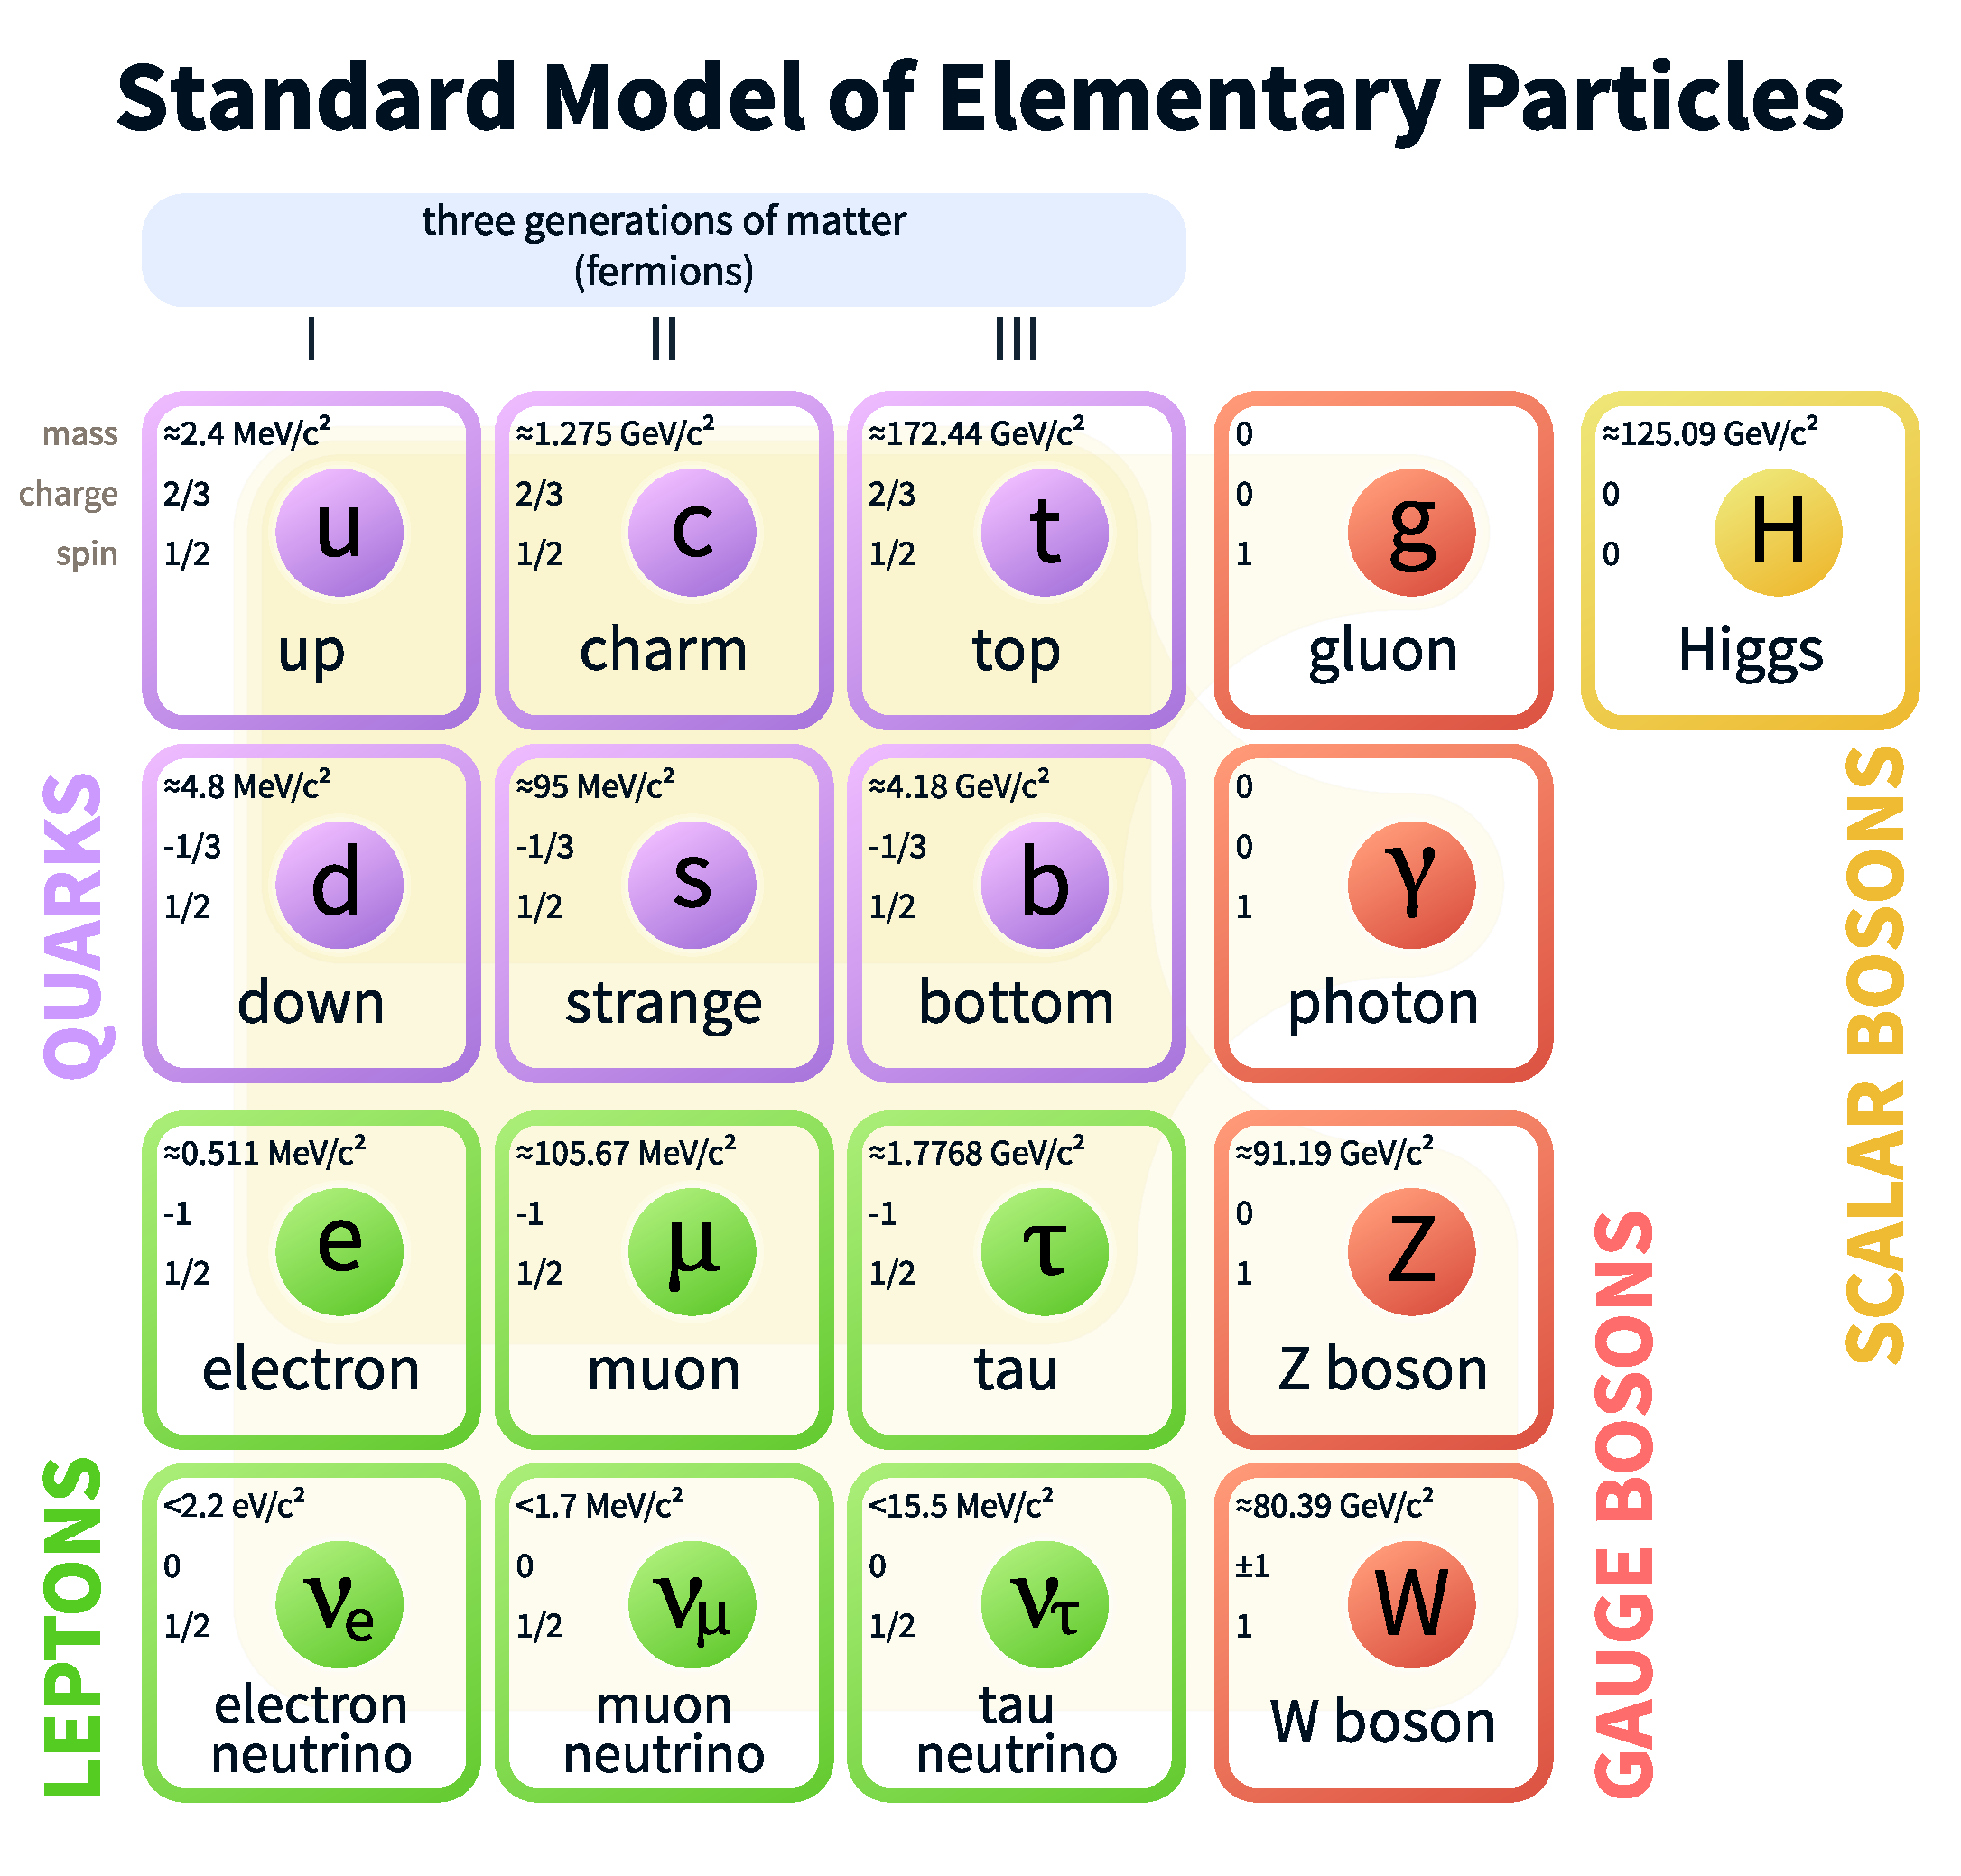
\includegraphics[width=0.9\textwidth]{intro/figs/Standard_Model_of_Elementary_Particles}
	\renewcommand{\baselinestretch}{1.0}
	\caption[An illustration of the elementary particles in the Standard Model and their properties.]{An illustration of the elementary particles in the Standard Model and their properties. The three left columns represent the different generations of fermions, with quarks in purple and leptons in green. The gauge bosons are represented in the fourth column in red, and the only scalar boson, the Higgs, in the fifth column in yellow. \cite{cc}}
	\label{fig:sm}
\end{figure}

\section{Issues with the Standard Model}
\label{sec:smIssues}

Despite the great success of the Standard Model in describing many of the fundamental interactions of particles, it is insufficient to explain all physical phenomena. There are several outstanding theoretical questions left unanswered by the Standard Model, and experimental evidence to suggest it is incomplete.

One of the most perplexing theoretical features of the SM is the fact that we have been able to detect all the elementary particles at energies accessible in our experiments. Because the bare masses of particles in the SM Lagrangian receive corrections from quantum loop diagrams, it is not clear why new particles (which must be massive) do not contribute significantly to these corrections. In particular, the quantum loop corrections to the Higgs boson mass include all massive particles, and contributions from undiscovered massive particles could drive the Higgs mass far beyond what is currently accessible, yet this is not observed. This is often referred to as the {\it hierarchy problem}.

Experimental evidence also suggests there are physical phenomena not explained by the SM. Measurements of the rotational velocity of galaxies compared to the visible matter indicate there is an abundance of {\it dark matter} in the universe which cannot be accounted for by the particle content of the SM \cite{Corbelli:1999af}. Furthermore, while the SM predicts neutrinos to be massless, measurements of neutrino flavor oscillations imply that neutrinos mass is very small, but nonzero \cite{Alberico:2003kd}. Such measured phenomena indicate there may be additional particle content beyond what is posited by the SM, and additional interaction terms between SM particles and a ``dark sector'' of weakly-interacting particles.

\section{Beyond the Standard Model: Supersymmetry}
\label{sec:bsm}

In order to solve many of the theoretical and experimental issues with the SM, theorists had considered extending SM particle content and interactions to include additional species which might satisfy some of the theoretical constraints of the SM in a consistent manner with observation. However, in 1975 the Haag-\L{}opusza\'{n}ski-Sohnius theorem \cite{Haag:1974qh} demonstrated that the only non-trivial extensions of quantum theories do not only include internal symmetries and the Poincar� symmetry, but also a non-trivial extension of the Poincar� algebra known as {\it supersymmetry} \cite{PhysRevD.3.2415, NEVEU197186, Golfand:1971iw, NILLES19841, FAYET1975104, WESS197439, WESS197452, Volkov:1972jx}.

A quantum field theory of supersymmetry (SUSY) can be visualized as a dual version of a typical field theory. For each particle, there exists a superpartner with different spin; fermions have boson-like superpartners and bosons have fermion-like superpartners. This is a particularly appealing and elegant solution to many of the issues with the SM; loop diagram corrections to particle mass are partially cancelled out by contributions from superpartner loop diagrams, providing a natural solution to the hierarchy problem \cite{Martin:1997ns}. In typical ``R-parity conserving'' SUSY theories, particle interactions also conserve ``SUSY-ness'' in decays, and thus when a superparticle decays into SM particles, the cascade will always end in the lightest supersymmetric particle (LSP). The LSP must be stable, and because it interacts very weakly with the SM sector provides a suitable dark matter candidate.

While there are many beyond-SM (BSM) theories that seek to explain phenomena beyond the scope of the SM, SUSY provides both elegant solutions to the theoretical concerns of the SM as well as a robust framework to unexplained physical phenomena. The analysis described here is designed to be model independent in a search for new physics, but also sets constraints on SUSY models as it is one of the more promising BSM theories that might be realized by nature.
% --------------------------------------------------------------------------- %
% --------------------------------------------------------------------------- %

% --------------------------------------------------------------------------- %
% --------------------------------------------------------------------------- %
\chapter{The Large Hadron Collider and the CMS Detector}
\label{ch:detector}

In order to probe the most fundamental constituents of nature, accelerators ramp particles up to great energies and then collide them to probe particle interactions. Detectors situated at the collision point can measure the outgoing products from particle collisions, and physicists can study the interactions to measure SM parameters, determine particle properties, quantify interaction rates, or search for new particles and processes.

The Large Hadron Collider is the most powerful particle accelerator ever constructed, and collides protons at a rate of nearly one billion times per second at a record energy of 13 Teraelectronvolts. The Compact Muon Solenoid is one of the all-purpose physics detectors that monitors the products of proton-proton collisions delivered by the LHC. Together with the ATLAS detector (A Toroidal LHC ApparatuS), the CMS detector is responsible for collecting data to measure a wide range of physics phenomena.

% --------------------------------------------------------------------------- %
% --------------------------------------------------------------------------- %
\section{The Large Hadron Collider}
\label{sec:lhc}

% --------------------------------------------------------------------------- %
% --------------------------------------------------------------------------- %

% --------------------------------------------------------------------------- %
% --------------------------------------------------------------------------- %
\section{The Compact Muon Solenoid}
\label{sec:cms}
The Compact Muon Solenoid (CMS) is a general-purpose physics detector at the LHC, situated at one of the five collision points along the main ring. The detector encapsulates the collision point with layers of various subsystems designed to interact with the outgoing particles of the proton-proton collisions, and measure the position and energies of the collision products. Because of the extremely high rate of interactions at the collision point (on the order of one billion interactions per second), saving data from every bunch crossing would be unsustainable, and so the detector is also equipped with a system of hardware and software implemented "triggers" which identify events of interest for physics analyses to be saved to disk for further analysis.

The physical construction of the detector is motivated by the different interaction of particles with different types of materials, and consists of several subsystems layered as coaxial cylinders around the interaction point. Each subsystem consists of (sometimes different) components covering the fiducial area coaxial with the beamline (the {\it barrel}) and also the ends of the cylinder (the {\it endcap}). The innermost subsystem of CMS is the silicon tracker, which consists of many layered silicon pixels designed to pinpoint the locations of charged particles while minimally interacting with the particle's trajectory. The layer beyond the tracker is the electromagnetic calorimeter (ECAL), a grid of lead-tungstate crystals which scintillate to measure the energies of electromagnetic particles. Beyond the ECAL is the hadronic calorimeter (HCAL), a sampling calorimeter designed to measure the energies of hadronic particles (which deposit minimal energy in the ECAL). The final, outer layer is the CMS muon detector, where the muon detection stations are interweaved with the magnetic return yoke that generates the toroidal 3.8T magnetic field inside the detector volume. The total dimensions of the detector are 21.6m long and 14.6m in diameter, weighing over 12,500 tons.

\subsection{Silicon Tracker} 
\label{subsec:tracker}
The silicon vertex tracker (SVT) is a series of silicon pixels and strips designed to measure the position of charged particles in the detector, while disturbing their path as little as possible. The position of particles in the interior is of particular importance in event reconstruction; charged particles traveling in a magnetic field will deflect in a curved path with radius proportional to the particles momentum as described in equation \ref{eq:momentum}, and so the track reconstruct can be used to not only determine a particle's momentum with high precision, but also the sign of its charge based on the direction of curvature.
\begin{equation}
	\label{eq:momentum}
	p = qrB
\end{equation}
As the innermost detector subsystem, the SVT experiences the highest flux of particle radiation. In the barrel region, the tracker layers are oriented in 3 coaxial layers. Closest to the interaction point where particle flux is the greatest, very precise silicon pixels are used, measuring $100\times150 \mu \text{m}^2$, whereas in other layers the flux is low enough to use microstrip detectors, measuring $10 \text{cm}\times80\mu \text{m}$ and  $25 \text{cm}\times180\mu \text{m}$ in the middle and outer layers respectively. In the endcaps, the pixel strips are arranged in a turbine-like pattern in two separate layers on each end. This configuration allows for the precise measurement of particle position for track reconstruction, while minimizing the amount of material which might deflect particles from their original trajectories. A partial geometry of the SVT layout can be seen in figure \ref{fig:pixelLayout}.
\begin{figure}
	\centering
	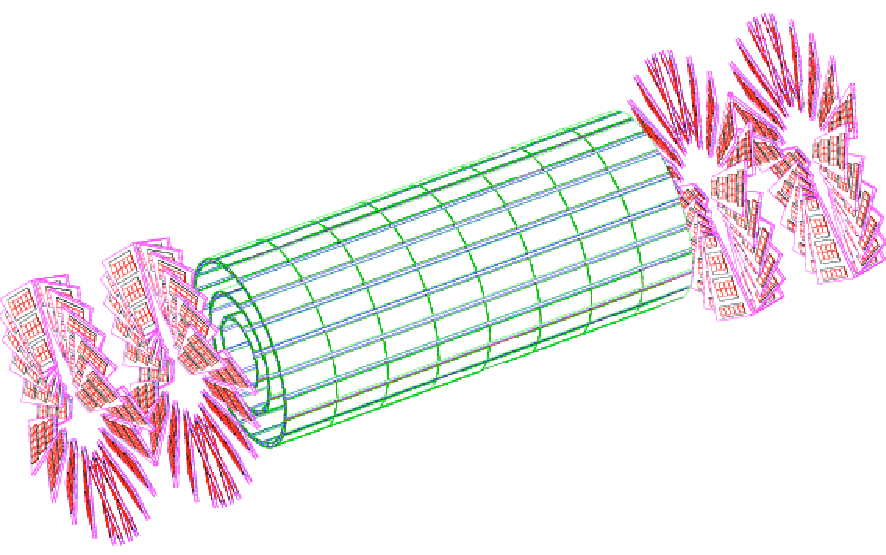
\includegraphics[width=0.95\textwidth]{detector/figs/trackerGeometry}
	\caption{Geometry of silicon tracker inner layers in CMS.}
	\label{fig:pixelLayout}
\end{figure}

\subsection{Electromagnetic Calorimeter}
\label{subsec:ecal}
The ECAL is used to measure the energies of particles which interact electromagnetically, both absorbing the incident particles and scintillating to provide an energy-readout to photodiodes attached to each crystal. Constructed of lead-tungstate ($\text{PbWO}_4$), electromagnetically interacting particles (such as electrons or photons) will interact with the crystal material, losing energy through a cascade of electromagnetic interactions including election-positron pair production and bremsstrahlung. This phenomenon --- also referred to as "showering" --- causes the crystals to scintillate proportional to the energy deposited in the crystal, which is then measured by various photodiodes to extract an accurate measurement of the particle energy, now fully absorbed by the calorimeter.
%\begin{figure}
%	\centering
%	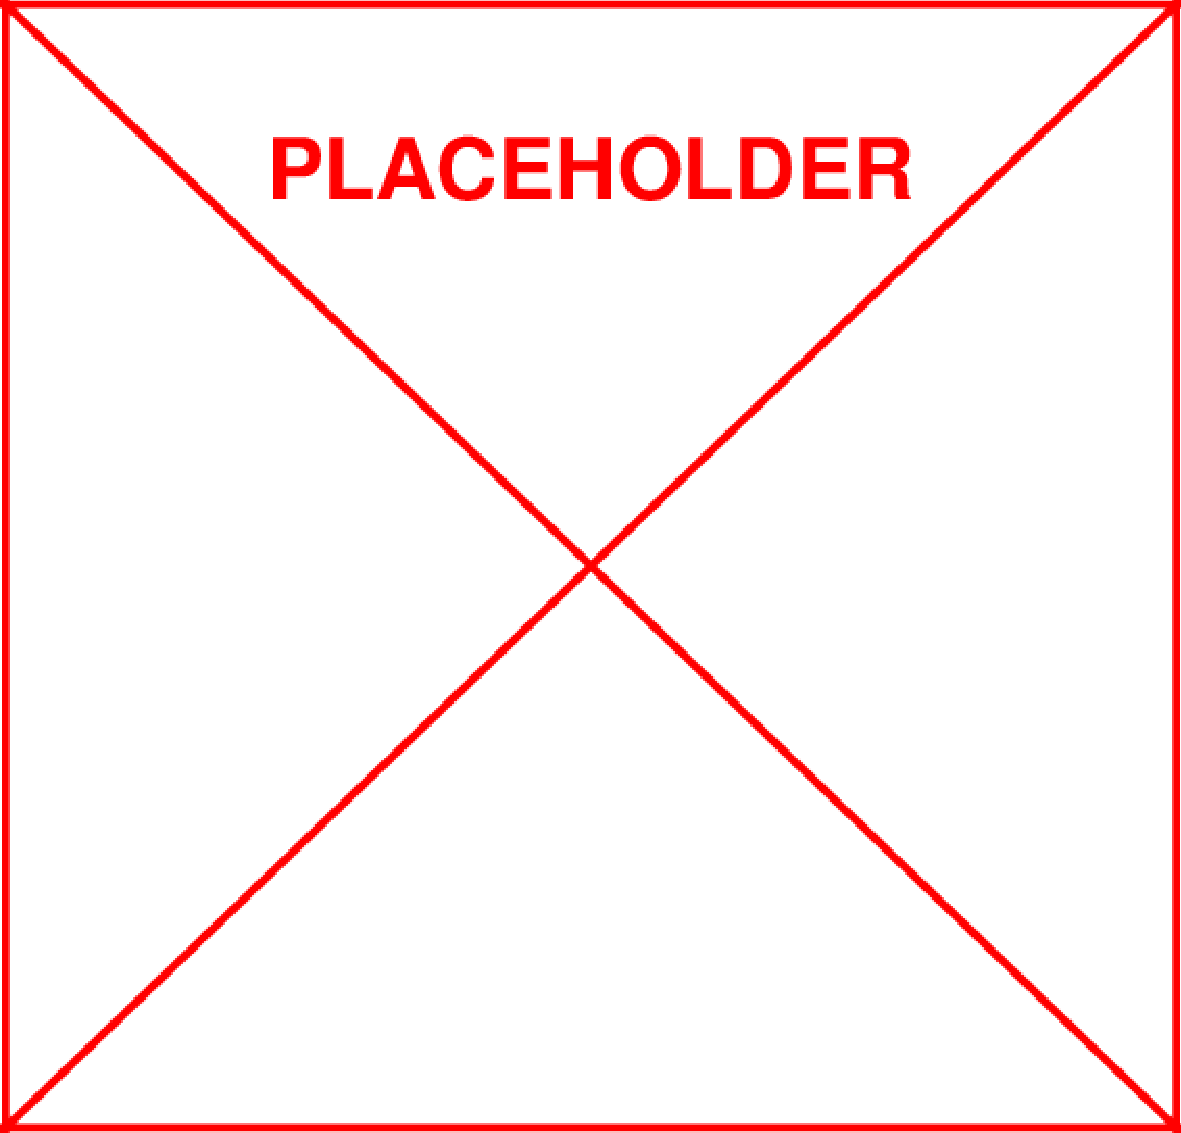
\includegraphics[width=0.4\textwidth]{figs/placeholder}
%	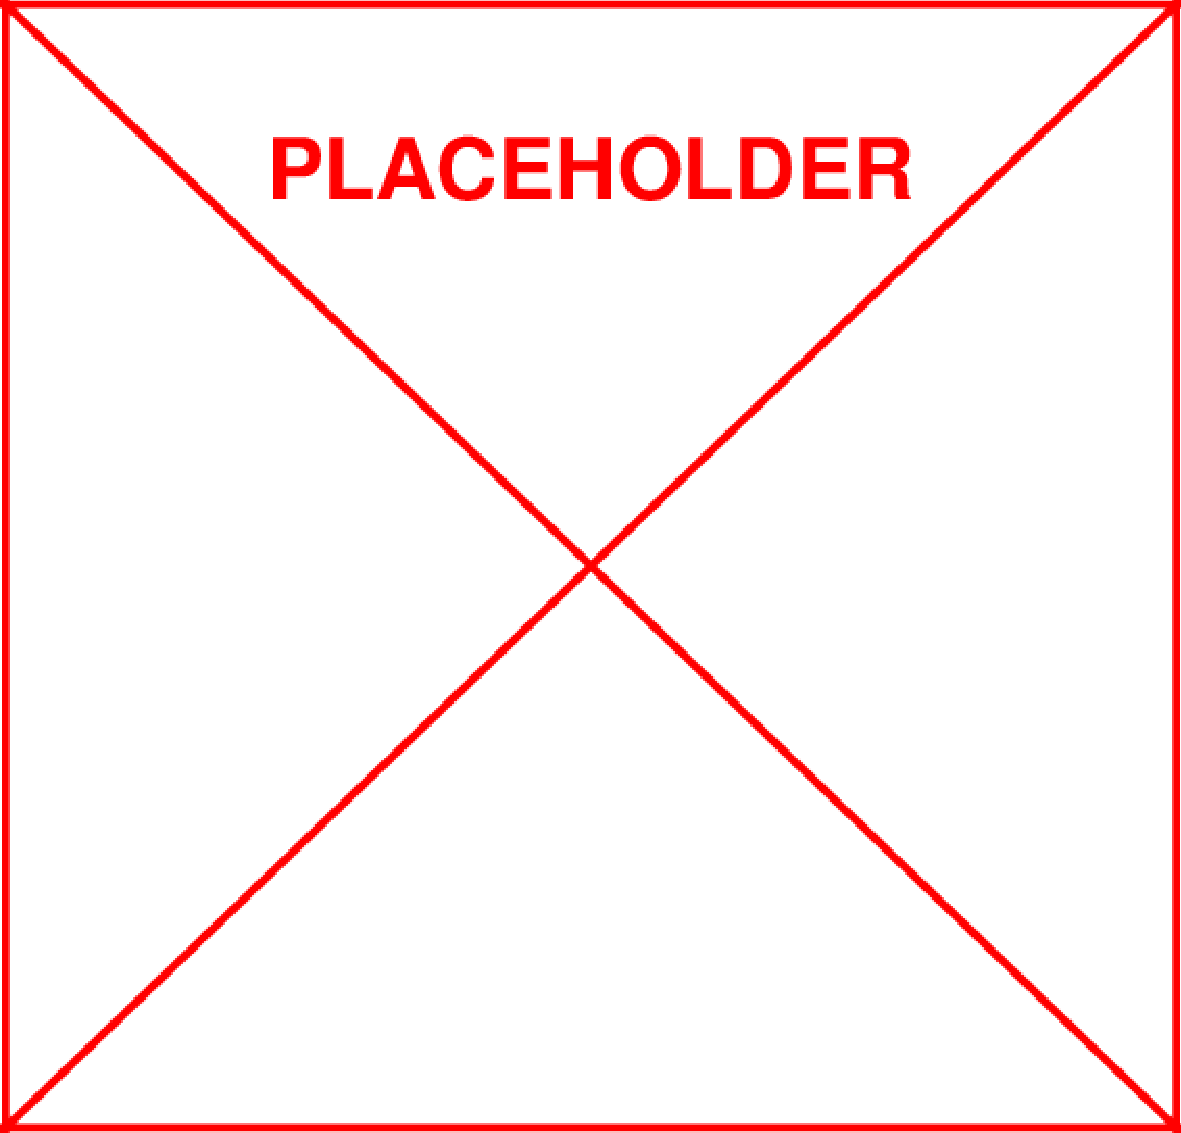
\includegraphics[width=0.4\textwidth]{figs/placeholder}
%	\caption{Feynman diagrams depicting the main processes by which particles shower in the ECAL. The left diagram depicts electron-positron pair production from a photon, and the right diagram depicts bremsstrahlung, where an electron radiates energy away through a photon.}
%	\label{fig:ecalFeynman}
%\end{figure}

The fundamental principle of the calorimeter measurement relies on the energy loss of particles interacting with matter. In general, the energy of a particle traveling a distance $X$ through some material is given by equation \ref{eq:energyDist}, where $E_0$ is the initial energy of the particle and $X_0$ is the material-dependent radiation length. 
\begin{equation}
	\label{eq:energyDist}
	E(x)=E_0 e^{\frac{-x}{X_0}}
\end{equation}
The design of the calorimeter is motivated by the choice of a scintillating, radiation-hard material with short $X_0$ such that incident electromagnetic particles deposit all their energy and are stopped by the ECAL. The resolution of the energy measurement is also dependent on the "stochastic term", which parametrizes the uncertainty due to statistical and measurement fluctuations in the calorimeter, and is given by equation \ref{eq:ecalSigma}, where $S$ is the stochastic term, $N$ the noise, and $C$ the constant term. 
\begin{equation}
	\label{eq:ecalSigma}
	\left(\frac{\sigma}{E}\right)^2=\left(\frac{S}{\sqrt{E}}\right)^2+\left(\frac{N}{E}\right)^2+C^2
\end{equation}
The energy resolution can be measured by a test beam of known energy, as shown in figure \ref{fig:ecalSigma}.
\begin{figure}
	\centering
	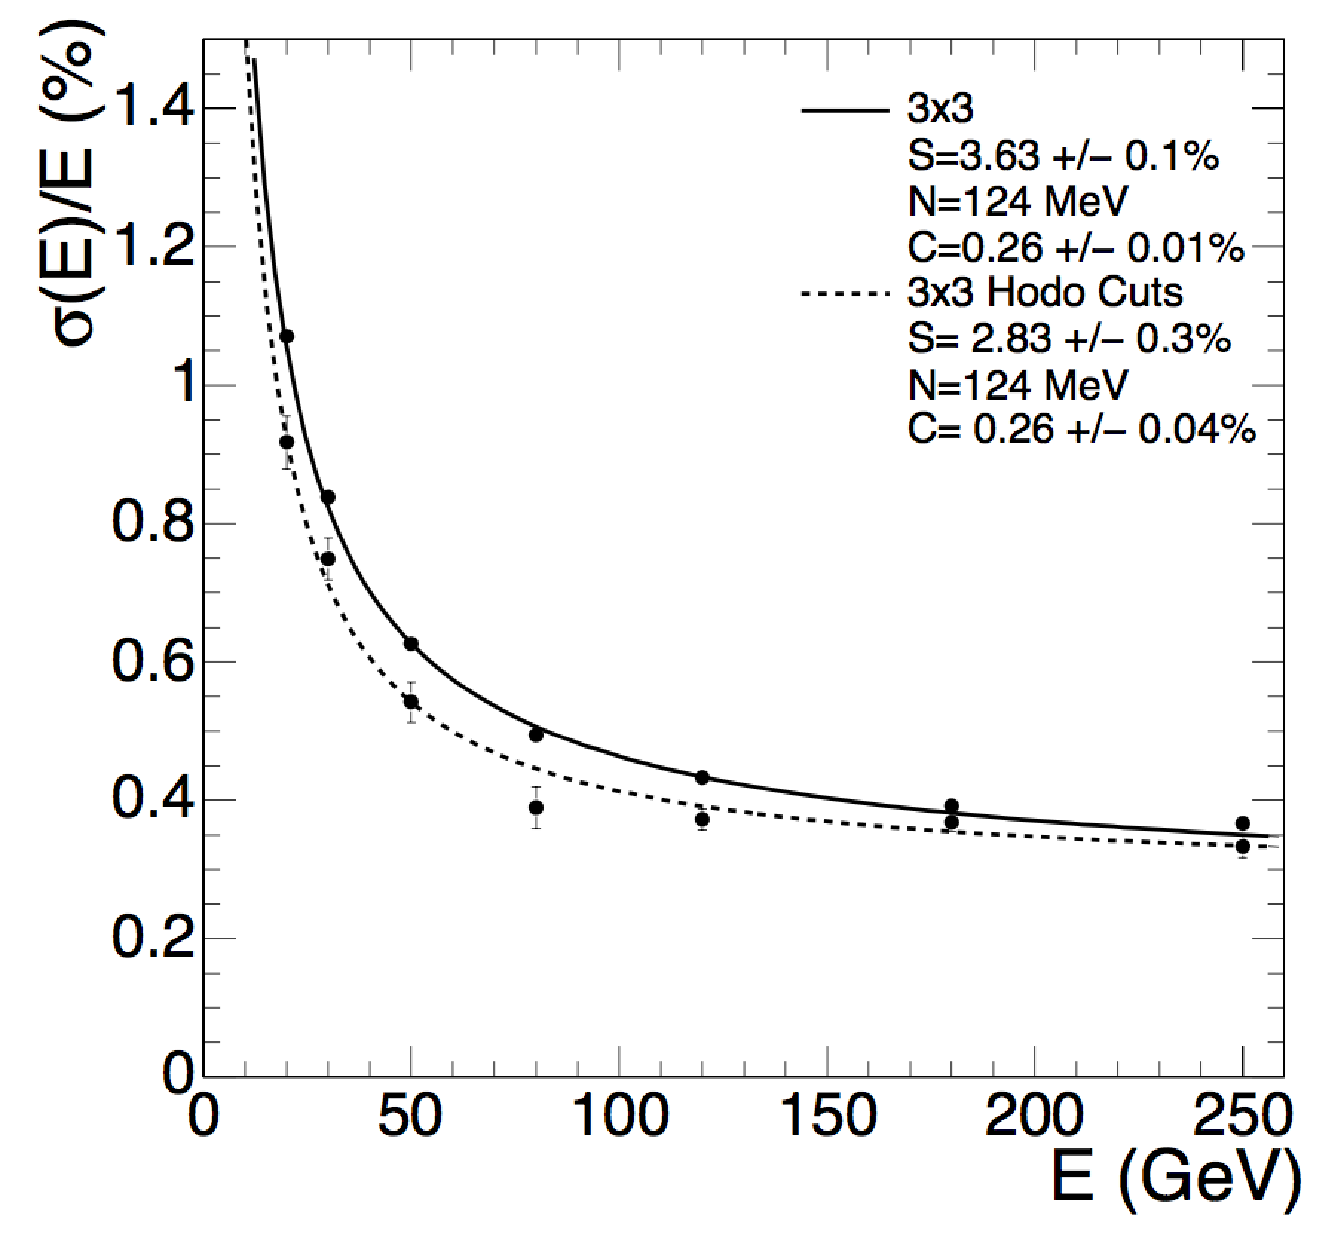
\includegraphics[width=0.65\textwidth]{detector/figs/ecalRes}
	\caption{Energy resolution $\sigma/E$ of the ECAL as a function of electron energy measured using a test beam. The energy was measured in a $3\times3$ crystal array with electrons incident on the center crystal, with electrons falling in a $4\times4\text{mm}^2$ region (lower points) and $20\times20\text{mm}^2$ region (upper points).}
	\label{fig:ecalSigma}
\end{figure}

The construction of the calorimeter is also divided into two sections by the cylindrical geometry, the ECAL barrel section (EB) and ECAL endcap sections (EE). The EB consists of 61,200 crystals arranged into 36 "supermodules", each spanning half the barrel length, and uses silicon avalanche photodiodes (APDs) as photodetectors. The individual crystals are tilted slightly (3\textdegree) in an $\eta-\phi$ grid with respect to the nominal interaction point, with a front-facing area of $22\times22\text{mm}^2$ and a length of 230mm. The EE instead uses vacuum phototriodes (VPTs) as photodetectors, and consists of approximately 15,000 crystals clustered in $5\times5$ units, also offset from the interaction point but arranged in an $x-y$ grid, with a cross section of $28.6\times28.6\text{mm}^2$ and a length of 220mm. The EE is also equipped with a "preshower" device placed in front of the crystal calorimeter, consisting of two strips of silicon strip detectors to enhance $\pi^0$ rejection. The layout of the ECAL can be seen in figure \ref{fig:ecalGeometry}. Because of the depth of the ECAL crystals (which are $\sim25X_0$, and the confining properties of the crystals (which have a Moliere radius of 2.2cm, the radius of a cylinder containing 90\% of a shower's energy on average), electrons and photons are typically well reconstructed in CMS, except in the transition region where EB and EE meet.
\begin{figure}
	\centering
	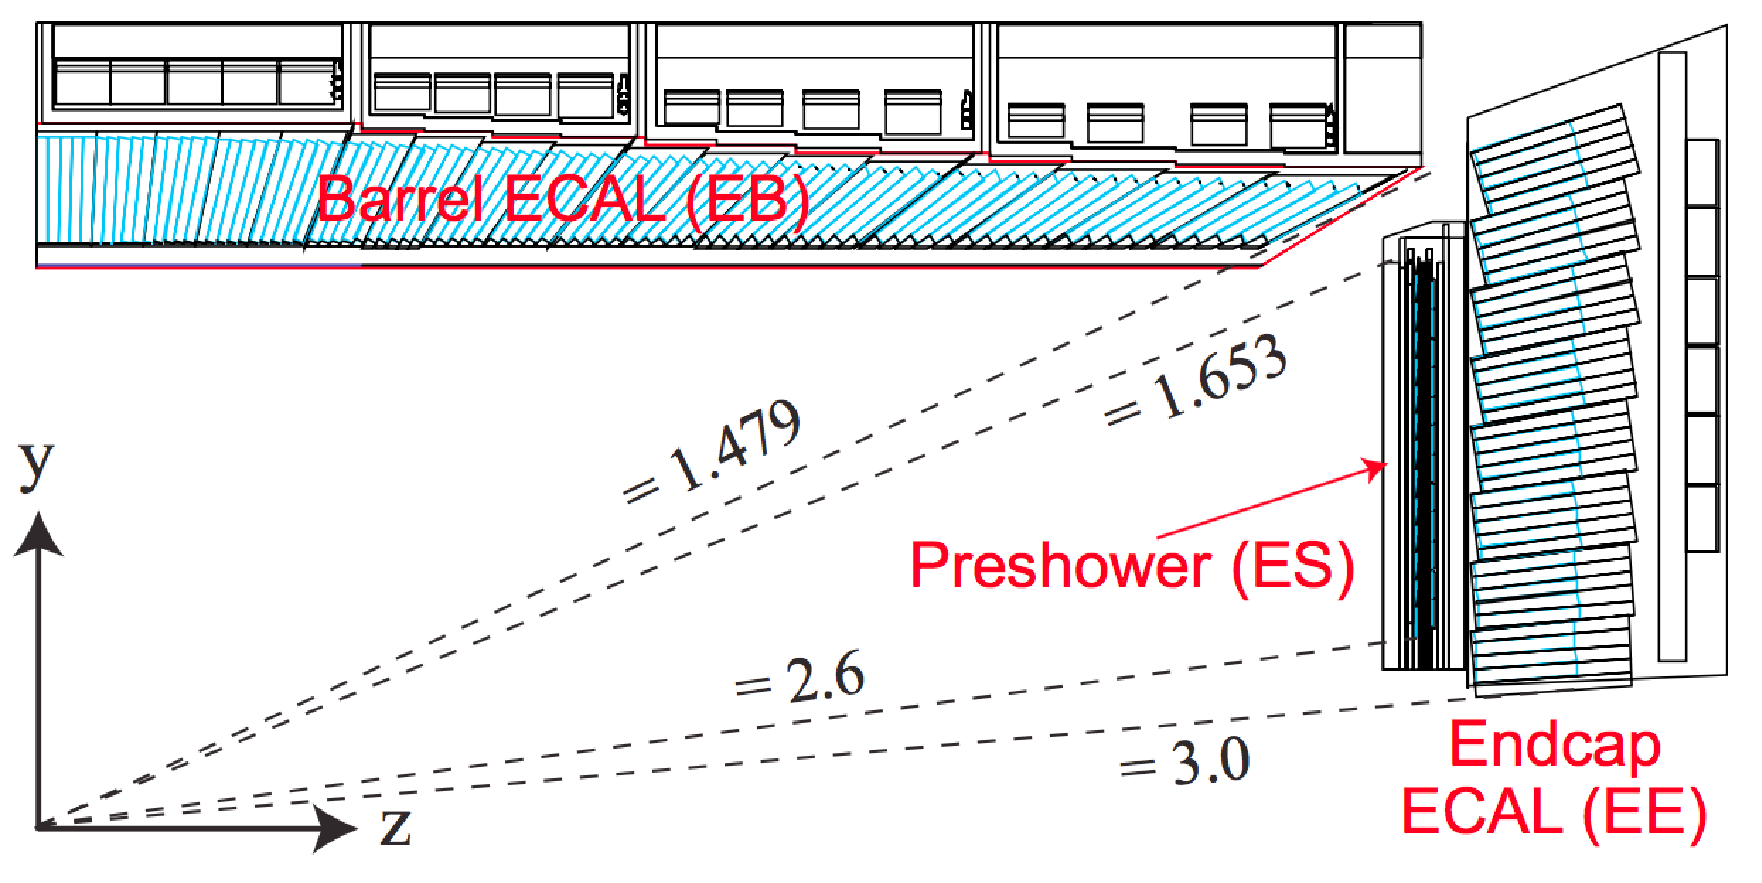
\includegraphics[width=0.95\textwidth]{detector/figs/ecalGeometry}
	\caption{A cross section of the ECAL geometry, with the dashed lines marking the pseudorapidity values $\eta$ covered by the various subsystems.}
	\label{fig:ecalGeometry}
\end{figure}

\subsection{Hadronic Calorimeter}
\label{subsec:hcal}
The CMS HCAL is a sampling calorimeter. Designed with alternating layers of scintillating and absorbing material, incident hadronic particles (such as charged pions, kaons, protons, etc.) interact with the absorber material and consequently shower into electromagnetic particles, whose energy can be read out by photodiodes connected to the scintillating material. Brass is used as the absorber material for both its interaction length and non-magnetic properties, and plastic scintillator tiles connected to embedded wavelength-shifting fibers carry the light to a readout system.

As with the ECAL, the energy loss of hadronic particles in the absorber is characterized by the (hadronic) interaction length and equation \ref{eq:energyDist}. However, unlike the ECAL, the HCAL contains both hadronic and electromagnetic showers. Electromagnetic particles generated in hadronic showers  often fail to escape the absorber layers, and thus some electromagnetic energy is lost in the absorbers. The CMS HCAL is sometimes referred to as a {\it non-compensating calorimeter} because it is not constructed to actively compensate for the energy lost to these electromagnetic effects and the energy measurements must be corrected offline, known as "jet energy corrections" (JECs).  JECs are typically calculated by examining data from collisions producing a boson recoiling against  hadronic particles. By accurately measuring the boson energy in the ECAL, the sum of the recoiling hadronic energy in the HCAL is inferred (by momentum conservation) and compared to the detector response. Because the performance of the HCAL can fluctuate with time and run conditions, JECs are regularly recalculated and applied to the raw energy measurements taken by the HCAL to compensate for these effects. Additional information on the corrections contained in JECs is detailed in section \ref{subsec:jets}. The energy resolution of the HCAL in different regions of pseudorapidity can be seen in figure \ref{fig:hcalSigma}.
 \begin{figure}
	\centering
	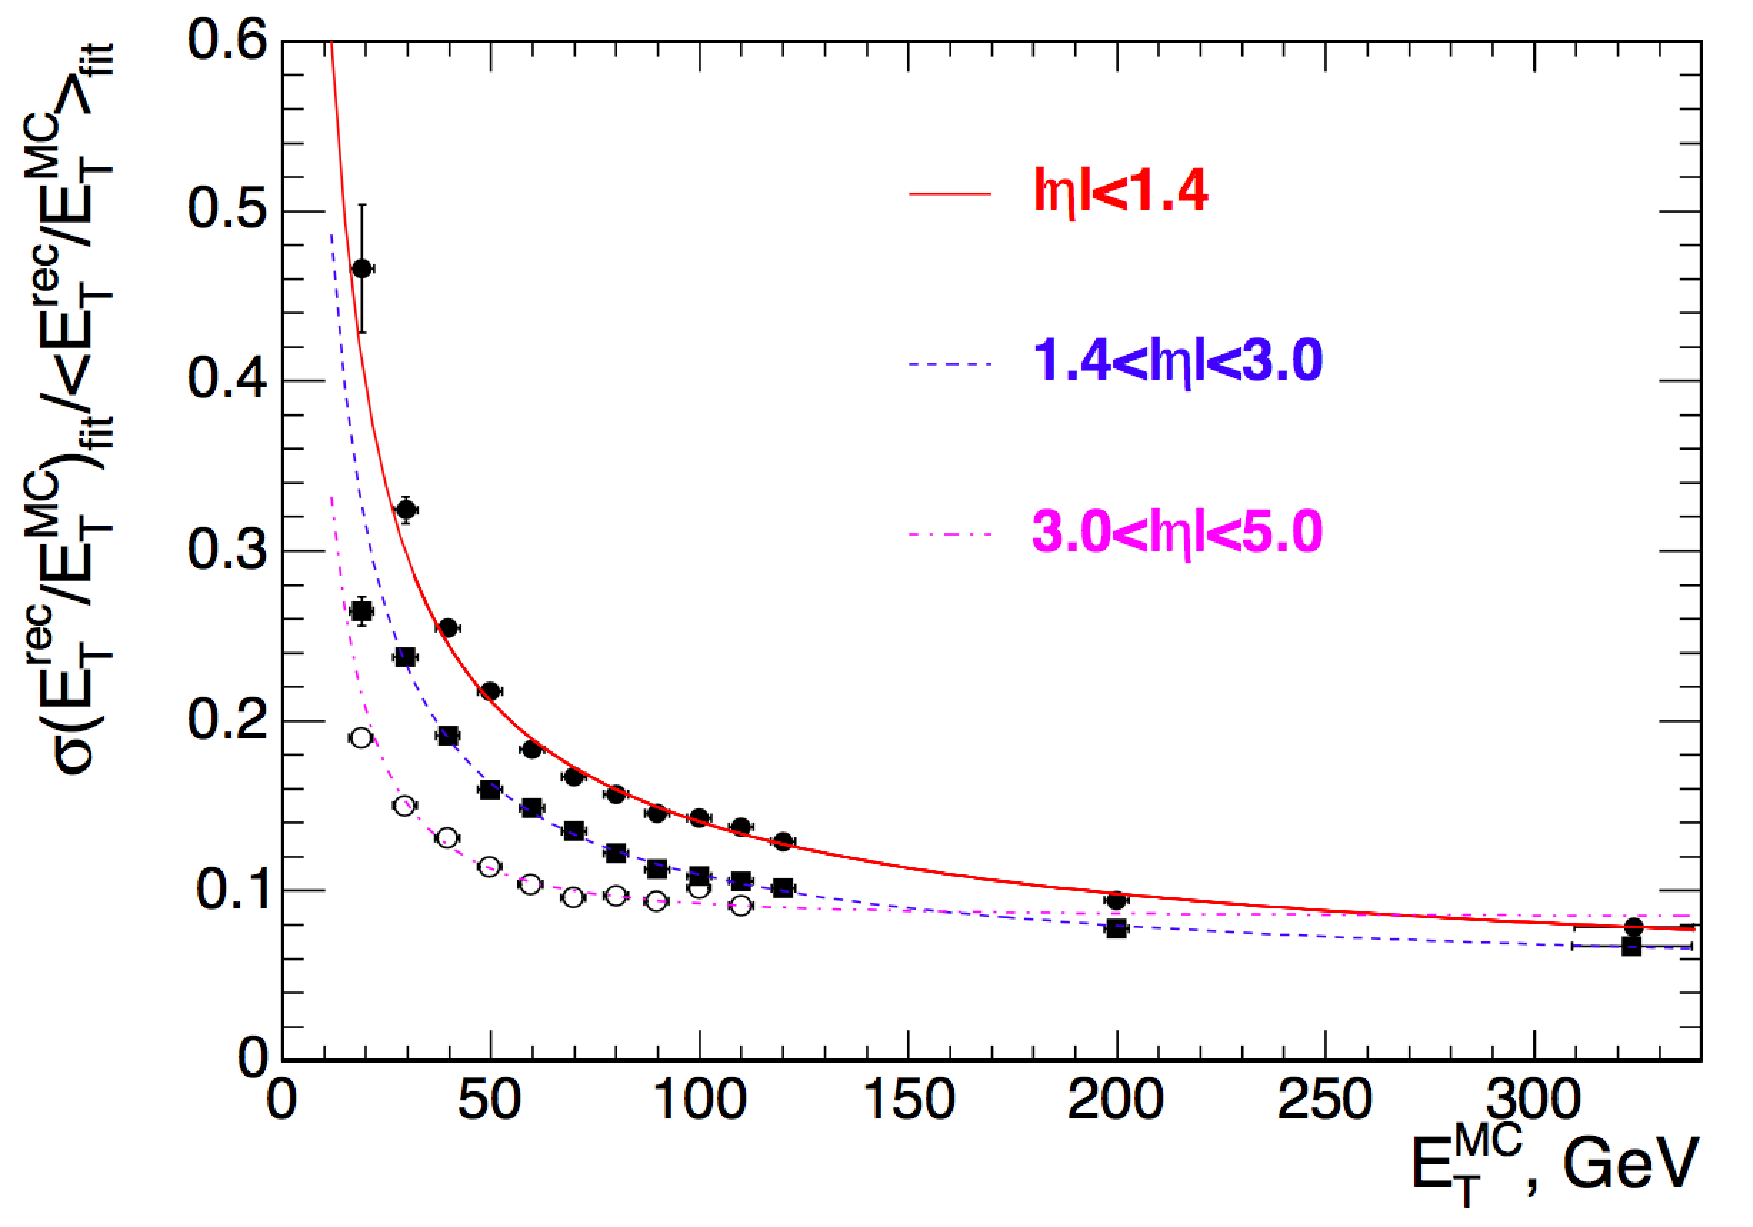
\includegraphics[width=0.75\textwidth]{detector/figs/jetEnergyRes}
	\caption{The jet transverse energy resolution as a function of the jet transverse energy, in different regions of pseudorapidity. For an explanation of jets, see section \ref{subsec:jets}}
	\label{fig:hcalSigma}
\end{figure}

The geometry of the HCAL can be reduced to four sections. The HCAL barrel (HB) consist of 32 "towers" of alternating absorber/scintillator material spanning the pseudorapidity region $-1.4<\eta<1.4$. The HCAL outer (HO) detector lies outside the vacuum tank of the magnetic coil and measures energy from any hadronic particles "leaking" through the HB, covering the pseudorapidity region $-1.26<\eta<1.26$. The HCAL endcap (HE) consists of 14 $\eta$ towers spanning the pseudorapidity range $1.3<|\eta|<3.0$. Finally, the HCAL forward (HF) is a different steel/quartz fibre calorimeter spanning the very-forward $3.0<|\eta|<5.0$ region. Instead utilizing Cherenkov radiation generated in the quartz fibers, the HF preferentially samples neutral hadronic energy and is ideally designed for the hadronic-heavy radiation environment in the forward region.

\subsection{Muon Detectors}
\label{subsec:muondetector}
The muon detector is the only subsystem which is constructed outside of the toroidal magnetic field. Interleaved with the magnetic return yoke, different muon detectors are used to aid in the identification and reconstruction of muon tracks. Because muons typically penetrate every other layer of the detector and have a large bending radius, additional measurements in the muon system --- combined with measurements in the SVT --- can lead to vastly improved resolution of muon momentum. The non-uniform magnetic field in the muon detector region (beyond the toroidal regime) causes an s-shaped trajectory and tighter bending radius (than in the SVT) for the muons, which improves the resolution for particles with transverse momentum above $\sim200\text{GeV}$ as seen in figure \ref{fig:muonSigma}.
 \begin{figure}
	\centering
	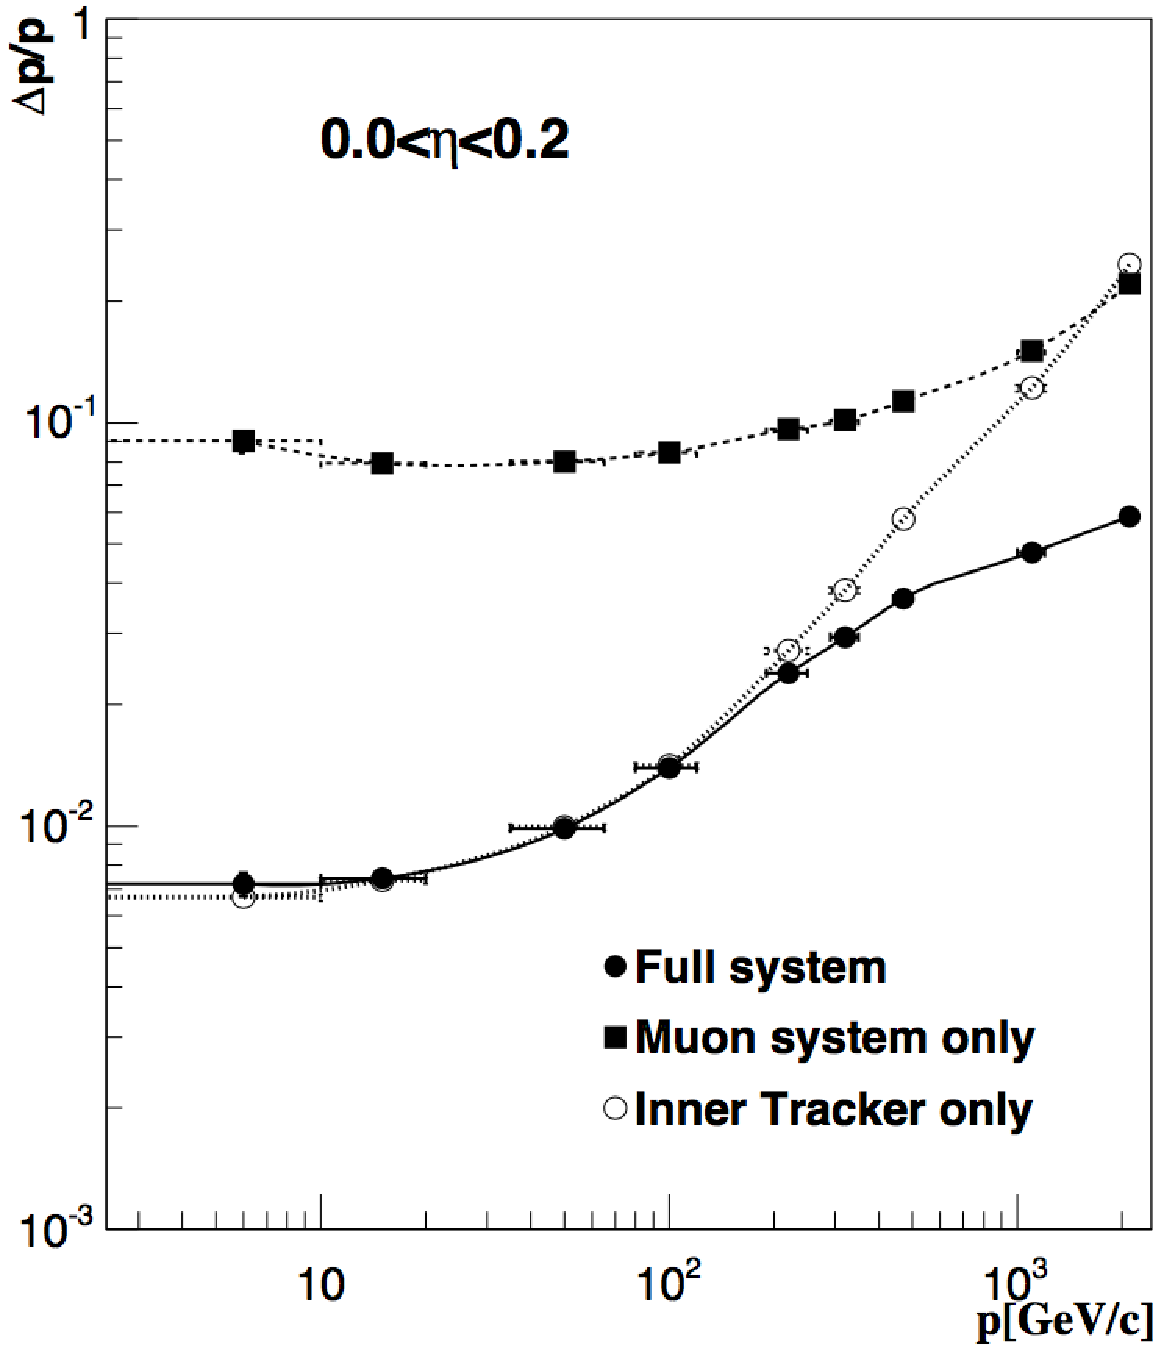
\includegraphics[width=0.45\textwidth]{detector/figs/muonResInner}
	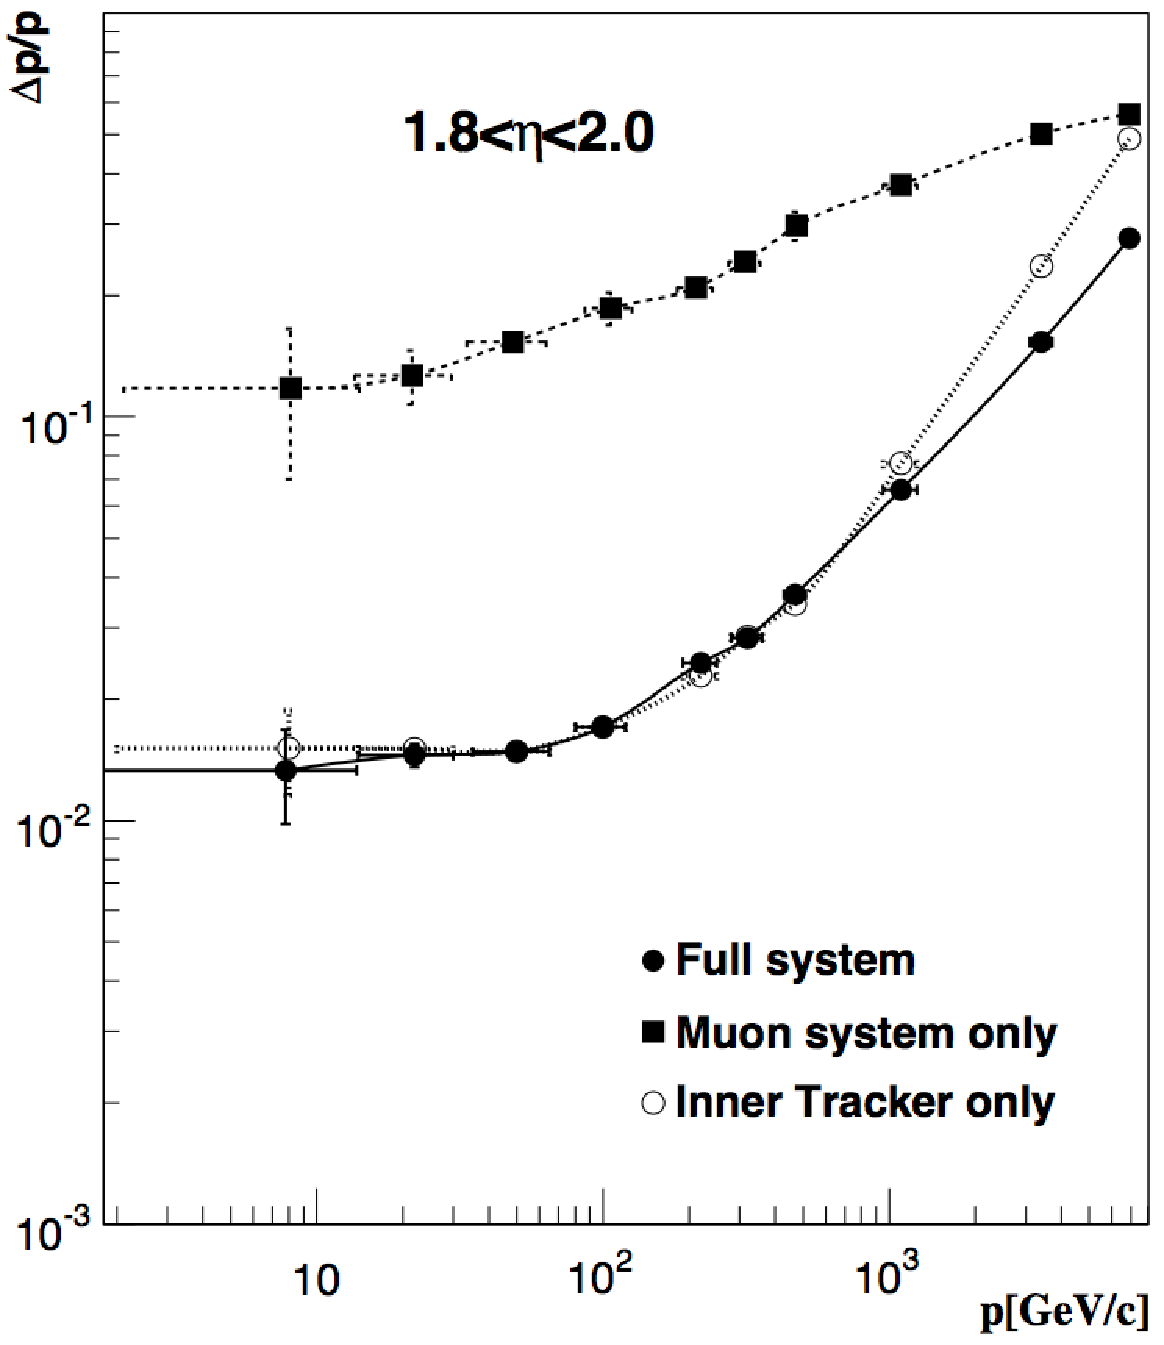
\includegraphics[width=0.45\textwidth]{detector/figs/muonResOuter}
	\caption{Muon momentum resolution as a function of muon momentum using only the inner tracking system, only the muon system, or both combined in the barrel region (left) or endcap region (right).}
	\label{fig:muonSigma}
\end{figure}

Different types of muon detectors are deployed (sometimes in combination) in different sections of the full muon system. In the barrel region ($-1.2<\eta<1.2$) where the muon flux, neutral background, and magnetic field are small, drift tube (DT) chambers are used. In the endcaps where the the muon flux, neutral background, and magnetic field are much greater, cathode strip chambers (CSCs) are used to increase coverage up to $|\eta|<2.4$. In addition to these technologies, both the barrel and endcap systems are supplemented with resistive plate chambers (RPCs) to provide complementary information to the DT and CSC detectors. The layout of the different muon detector components in the barrel and endcap can be seen in figure \ref{fig:muonGeometry}.
 \begin{figure}
	\centering
	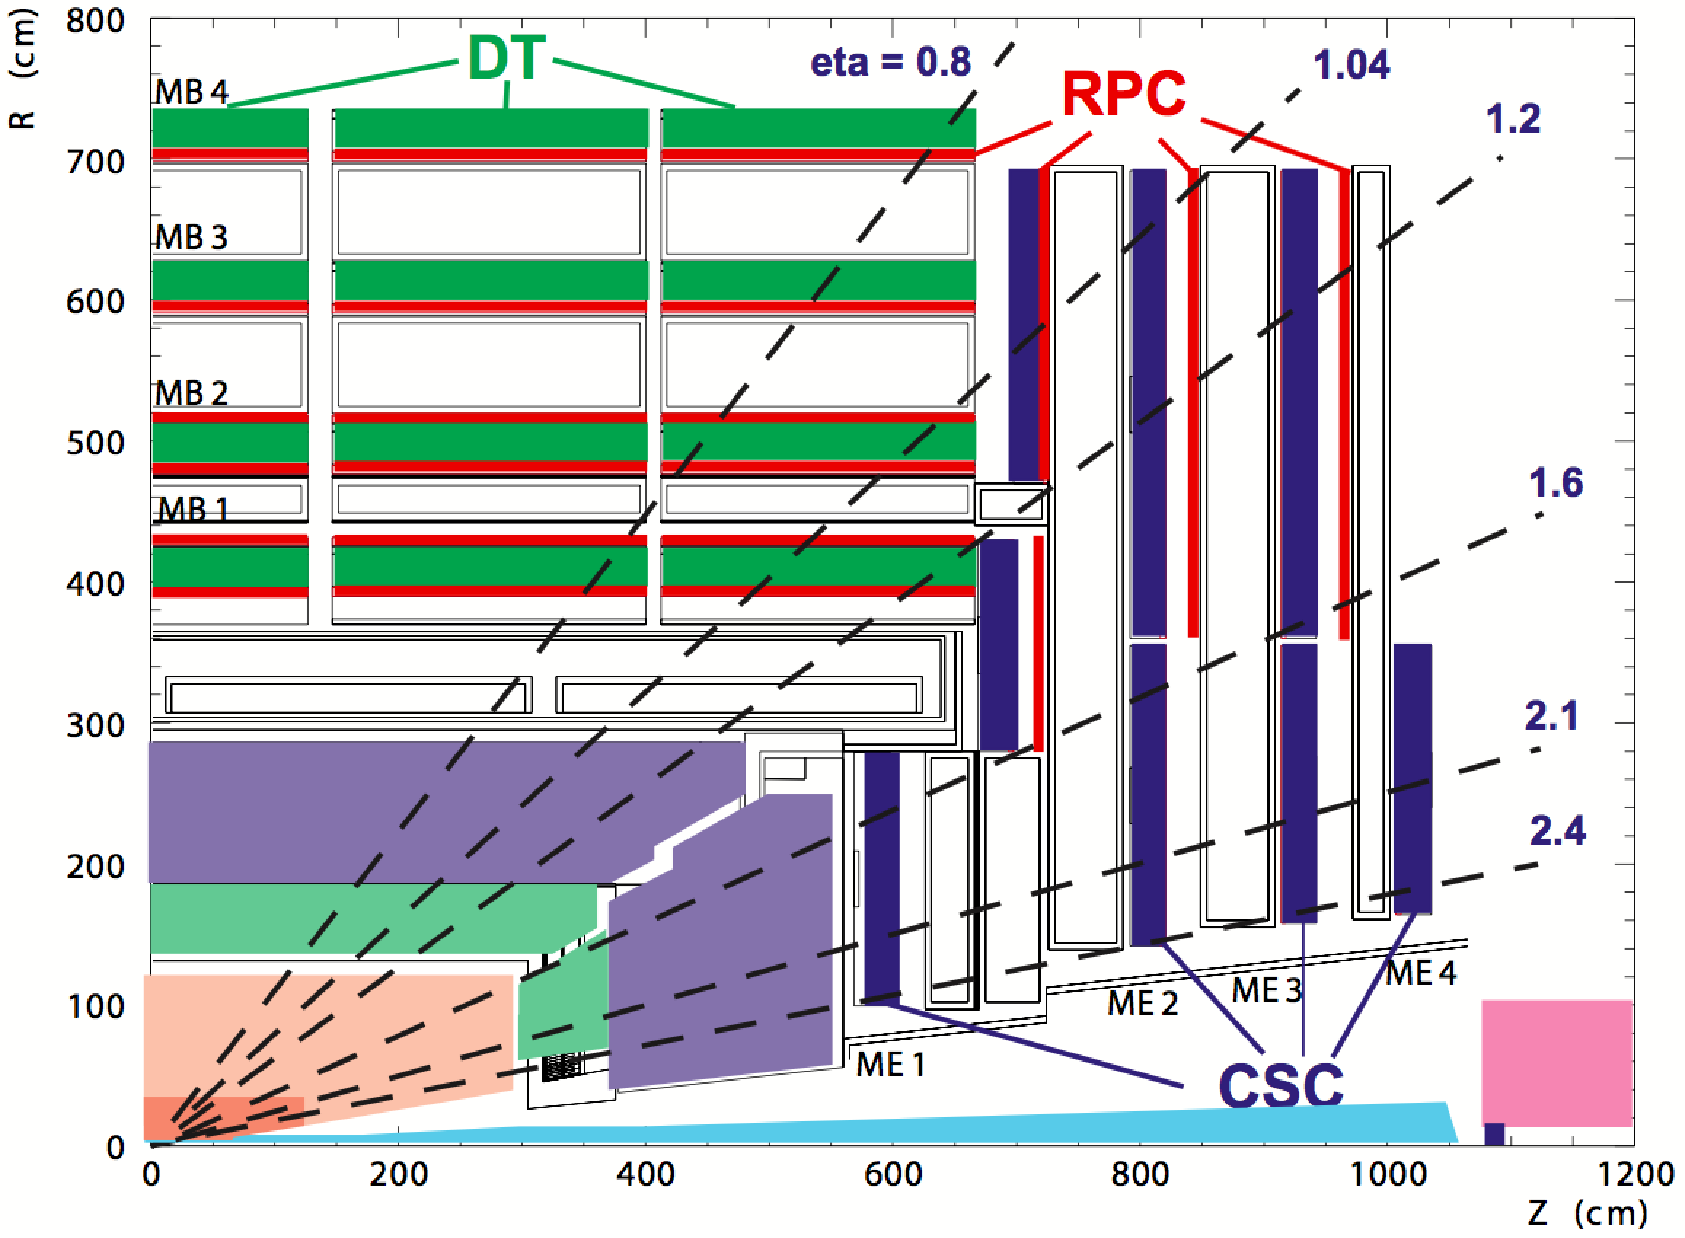
\includegraphics[width=0.75\textwidth]{detector/figs/muonGeometry}
	\caption{Layout of the CMS muon system for initial run configurations. The DT system is used only in the barrel region and CSCs in the endcap region, while RPCs are deployed in both the barrel and endcap.}
	\label{fig:muonGeometry}
\end{figure}

The DT detectors are chambers filled with gas surrounding a wire, with a voltage difference between the wire and outside of the DT. When charged particles pass through the drift chamber, they ionize the gas, and the ionization products will drift across the voltage difference in the tube, resulting in a detectable voltage change in the DT. By measuring both the position along the DT wire where charge is deposited, as well as reconstructing the "drift time" it takes for the ionized particles to reach the wire, DTs provide a 2-dimensional measurement of a particle's position. In CMS, the DT chambers consist of a dozen layers arranged into 3 groups, each with up to 60 DTs. The layers are arranged in such a way that some measure the direction of the muon parallel to the proton beam and others along the perpendicular coordinate, such that the full muon trajectory can be reconstructed by using the DT station information.

The CSCs in each endcap are trapezoidal in shape and overlap in the phi coordinate, increasing the fiducial coverage of the muon system. Each CSC consists of 6 gas gaps, where each gap is comprised of radially aligned cathode strips and a plane of anodes wires nearly perpendicular to the strips. When a muon passes through the CSCs, the ensuing ionization and electron avalanche deposits a charge on the anode wire and an image charge on the cathode strips. A measurement of the muon position can be reconstructed by determining the center-of-gravity of the charge distribution on the cathode strips, and the fast readout of the anode wire is used in low-latency trigger decisions as described in section \ref{subsec:triggers}.

The RPCs are complementary systems in both the barrel and endcap used to improve the time resolution of muon measurements. Each RPC consists of two parallel anode and cathode plates, separated by a gas chamber. The ionization of the gas as muons travel through the chamber is quickly deposited on the plates, and used for a precise time measurement of the muon crossing. Though the spatial resolution of the RPCs is poor, in conjunction with the other muon systems they allow for an unambiguous association of muons with different bunch crossings.
 
\subsection{Trigger Systems}
\label{subsec:triggers}
When operating at design luminosity, the LHC can deliver proton bunches to the collision point at a rate of 40MHz (or 25ns between bunches), resulting in an average collision rate on the order of one billion collisions per second. In order to achieve reasonable rates of data collection for offline storage and processing, the detector must suppress the event rate by six orders of magnitude when selecting events of interest to be saved for physics analyses. This is accomplished through a combination of readout electronics and the trigger systems: the Level-1 trigger (L1) processors and online High-Level triggers (HLT).

The L1 trigger system is comprised of specialized hardware processors to rapidly pre-select events of interest based on the calorimeter and muon systems. Based on the beam crossing frequency, the L1 electronics have only a few microseconds to collect readout data from the front end electronics and execute logic to select events of interest, such that the total time allotted for L1 trigger calculations is $<1\mu s$. During this time the bulk of detector data is held in a buffer while L1 trigger decisions are made based on data with reduced granularity and resolution rapidly collected from the calorimeter and muon systems, where triggers typically check for "trigger primitive" objects (such as photons, muons, electrons, etc.). Trigger primitives must meet certain momentum or energy thresholds, and L1 triggers may also check global data about the event such as the sum of transverse energy or the missing transverse energy (inferred from momentum conservation). 

After an L1 trigger tags an event, high-resolution data is read out from buffers for additional data processing before reaching the HLT. Each event of $\sim1.5MB$ is transferred to front-end readout buffers which then pipes data to a processor containing the HLT code. HLT code is designed to discard events as soon as possible when making trigger decisions and only a subset of objects or partial reconstruction of events may occur before the final trigger decision is made, though HLT algorithms typically approach the quality of final reconstruction. The HLT reduces the L1 output rate to $\mathcal{O}(100\text{Hz})$ for event storage and full reconstruction.
% --------------------------------------------------------------------------- %
% --------------------------------------------------------------------------- %

% --------------------------------------------------------------------------- %
% --------------------------------------------------------------------------- %
\section{CMS Physics Objects}
\label{sec:physicsobjects}

When physics events are fully reconstructed, detector data is used to identify {\it physics objects} representing real particles and event quantities for use in a physics analysis. The physics objects in an event --- such as leptons, jets, or missing energy --- and their properties are used to select events of interest for physics analyses targeting different final states. The properties of physics objects and global event data are also be used to make analysis level decisions of the quality of different objects. Here we describe some of the physics objects referred to in the \mttwo analysis and how they are reconstructed, as well as some global event properties and quality variables used as discriminants for physics objects and events.

\subsection{Particle Flow}
\label{subsec:pf}
Most of the physics objects described in the following sections are reconstructed and identified in CMS using the particle flow (PF) algorithm \cite{Sirunyan:2017ulk}. The PF algorithm is a holistic, iterative algorithm which uses all the available data in the detector to classify "PF candidate" particles in an event. PF works iteratively by identifying tracks and calorimeter deposits into a PF candidate, removing all energy and hits associated with the candidate and repeating the algorithm until all the detector information has been associated to PF objects. First any muon tracks in the inner tracker associated with muon system hits are associated and removed. remaining tracks are extrapolated into the calorimeters, and any energy deposits on the path are associated with the track and removed from further consideration. Once all the tracks have been associated, the remaining energy clusters can be identified with photons and neutral hadrons (depending on their presence in the ECAL or HCAL, respectively). An example of the different tracks and energy deposits associated with various particles can be seen in figure \ref{fig:pfCandidates}.
\begin{figure}
	\centering
	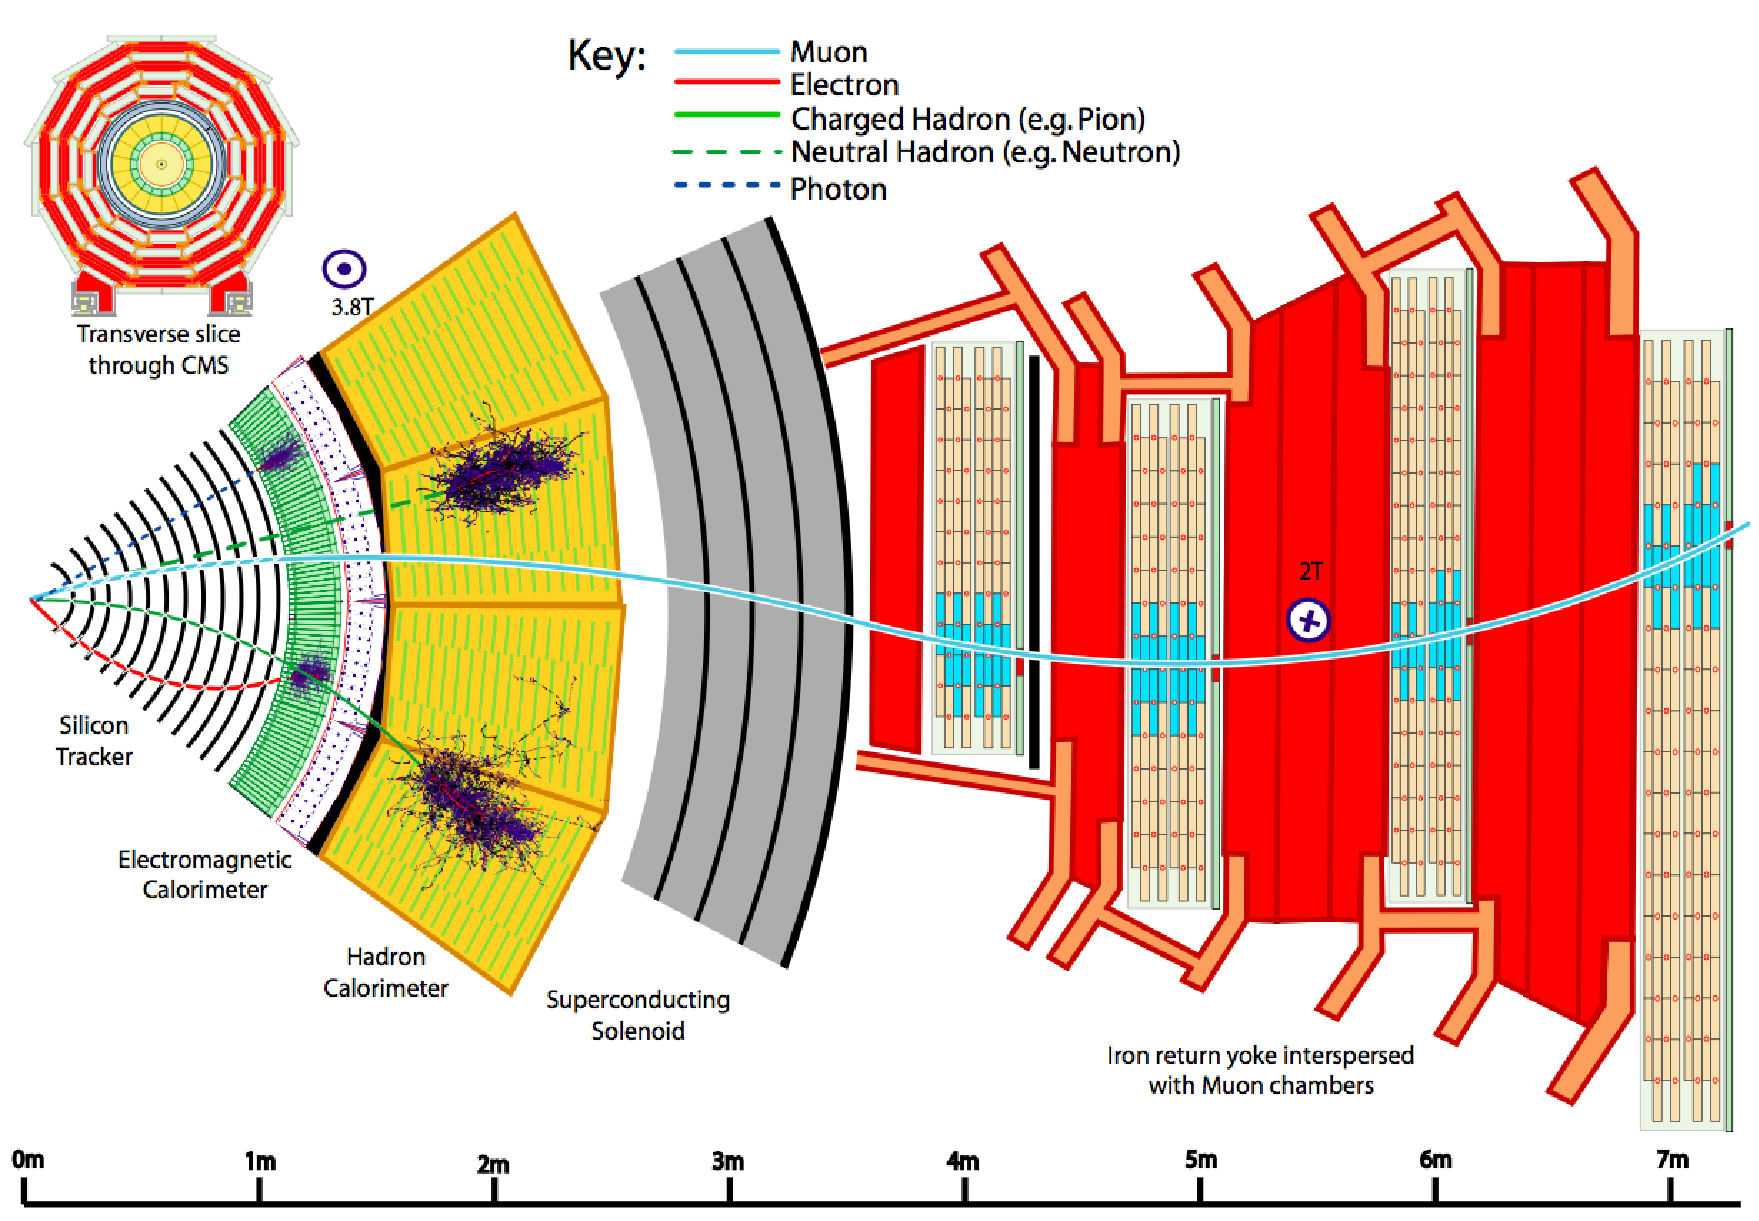
\includegraphics[width=0.95\textwidth]{detector/figs/CMS_Slice_2}
	\caption{A graphic depiction of different particles leaving various signatures in the different CMS detector subsystems. Particles may be detected via tracks hits, energy deposits, or a combination of both.}
	\label{fig:pfCandidates}
\end{figure}

\subsection{Isolation}
\label{subsec:iso}
Isolation is an important distinguishing variable for physics objects measured in the detector. Simply put, isolation measures the total amount of energy in some proximity to a physics object. Because many physics processes results in particle production outside the primary interaction vertex (such as showering, decays, hadronization, pair production, etc.), the isolation of a particle parametrizes the amount of other "activity" surrounding the physics object, and consequently proves a useful discriminant when determining if particles are produced in the primary interaction, or in subsequent physics processes. Particles which are produced in the primary physics process in a collision are sometimes referred to as {\it prompt}, and isolation is a powerful tool in identifying prompt leptons in particular.

\subsection{Electrons, Muons, and Photons}
\label{subsec:lepgamme}
The primary leptons considered in this analysis are electrons and muons (discussed in section \ref{subsec:muons}), and photons are also used as a cross-check in some control regions for background estimates. Prompt electrons and photons are identified in CMS primarily through the use of the ECAL, where they are stopped and deposit all their energy \cite{Baffioni:2006cd,Khachatryan:2015iwa}. Prompt electrons are customarily distinguished by both the presence of a track originating at the primary vertex and a sufficiently low isolation.

Electrons in CMS are identified primarily through the existence of a charged particle track terminating in an energy cluster in the ECAL. As described in section \ref{subsec:ecal}, the ECAL crystals are $\sim25$ radiation lengths deep, and will stop and contain nearly all of the energy of an electron (except perhaps minuscule losses to scattering in the tracker). The charged track leading to the energy deposit distinguishes the charged particle from a neutral particle, and the direction of curvature of the path in the tracker can be used to identify the charge of an electron (or positron).

Photons are distinguished from electrons by the lack of a track in the SVT. As a neutral particle, the only sign of a photon will be the energy deposit in the ECAL where the photon is stopped and deposits all its energy. Photons are typically distinguished from other neutral electromagnetic particles (such as a $\pi^0$) by the shape of the shower in the ecal. Whereas photons typically shower through pair production and bremsstrahlung, other hadronic particles may cascade via different physics processes leading to measurable difference in the shape of the energy cluster.

\subsection{Muons}
\label{subsec:muons}
Prompt muons produced in collisions at the LHC are generally minimum ionizing particles, and will penetrate the bulk of the detector. Without any matching calorimeter deposits, they are reconstructed using hits in the muon system matched to inner tracker hits \cite{Chatrchyan:2009ae}. The muon system flags muon candidates, which are then matched to inner tracker hits for the best fit of the muon track. Given the track hits, the transverse momentum and energy of the muon can be calculated by a fit to the track parameters. As with electrons, muons are customarily distinguished by both the presence of a track originating at the primary vertex and a sufficiently low isolation.

\subsection{Jets}
\label{subsec:jets}
Many particles produced at the LHC are created through the strong interaction, which may produce particles carrying color charge in the final state (i.e. quarks or gluons). Colored particles cannot exist individually due to the phenomenon known as {\it confinement}, and so via the process of {\it hadronization} (also refered to as {\it fragmentation}) they will proliferate in a series of interactions producing additional particle-antiparticle pairs, cascading in a parton shower to form hadronic bound states. When a "bare" quark or gluon is produced in the primary interaction, the ensuing hadronization results in a stream of tightly collimated hadrons aligned with the trajectory of the original bare particle, referred to as a {\it jet}. 

Jets present themselves in CMS as collimated energy deposits in both the ECAL and HCAL, as well as tracks originating at the primary vertex \cite{Schroder:2015czj}. Between the two calorimeters, all the electromagnetic and hadronic components of the jet are stopped and measured by the calorimeters, and any leptons (including muons detected in the muon system) which originate in the cone of the jet are assigned to the total jet energy. The jets are reconstructed using the "anti-k$_T$" algorithm, which clusters jet activity in cones of a fixed radius \cite{Cacciari:2008gp}. The jet is treated as a single physics object with a total energy equal to the sum of its electromagnetic, hadronic, and leptonic components, which by momentum conservation dictates the energy of the prompt quark or gluon that was produced in the primary interaction. 

Furthermore, the substructure of jets and their content can be analyzed to determine the flavor of the parent parton, known as "tagging". Jets are typically tagged to distinguish between those originating from heavy-flavor quarks (bottom or charmed) and light-flavor quarks. Top quarks produced in primary interactions are unique because of their short lifetime. A top quark will decay before hadronization occurs, instead producing a $W$ boson and down-type (down, bottom, or strange) quark which will subsequently hadronize. Searches involving top quarks in the final state typically employ "top-taggers" to search for these signatures of the top quark.

In practice, jets are complicated objects consisting of many constituent particles, and must be clustered and calibrated so that the jet energy closely matches that of the parent parton which produced the jet. Jet energy corrections (JECs) are applied to raw jet energies to compensate for different experimental deviations from the parent parton energy \cite{Khachatryan:2016kdb,CMS-DP-2016-020}. In particular, JECs include corrections to compensate for pileup energy as described in section \ref{subsec:pileup} \cite{Cacciari:2007fd}, detector effects (as a function of $\eta$), energy scale as a function of jet \pt, and residual corrections to account for differences between data and simulation. The JECs are calculated by collecting data events with a Z boson (decaying to electrons or muons) or photon recoiling against a jet. By precisely measuring the bosons energy with the ECAL, scale factors are derived for jets as a function of pseudorapidity $\eta$ and momentum \pt. 

\subsection{Missing Energy}
\label{subsec:met}
Missing energy refers to the sum of all energy which has escaped the detector, and is inferred from a momentum-imbalance in the physics objects measured by the detector \cite{Chatrchyan:2011tn}. Because the momentum of the incident protons is zero perpendicular to the direction of the beam, the momentum of physics objects produced in any collision must sum to zero in the direction transverse to the beamline. The missing transverse energy (\MET), is calculated by taking the negative vector sum of all PF candidates as in equation \ref{eq:met}. \MET is of particular importance to analyses targeting BSM physics, as BSM signatures characteristically contain invisible particles in the final state which escape detection.
\begin{equation}
	\label{eq:met}
	\vec{E}_T^{miss}=-\sum_i^{} \vec{p}_T^{\: i}
\end{equation}

The missing energy in an event is inferred from all other measured quantities in an event, and there are many sources of \MET which are unphysical in nature but rather dependent on experimental effects. Particles from the primary interaction with a sufficiently large pseudorapidity may escape the fiducial region of the detector subsystems, and resolution effects or intrinsic noise in the detector may lead to fluctuations in measured energies. These experimental effects must be suppressed or distinguished from "real" \MET due to physics processes creating particles which escape the detector (e.g. neutrinos). Analyses sensitive to final states with \MET often employ robust data-driven methods to predict or suppress backgrounds which might generate experimental sources of \MET or physics processes which can contribute real \MET (such as \znunu).

\subsection{Monte Carlo Simulation}
\label{subsec:simulation}

Monte Carlo (MC) simulation of events within the CMS detector is frequently generated to understand the expected physics, design analyses, and help predict certain backgrounds. The simulation begins with the underlying physics process of interest, and subsequently models the trajectories of particles in the final state through the detector volume, their interactions in those volumes and with the detector material, the effects of pileup, and the detector response.

The process of generating MC proceeds in multiple steps interfacing different software packages. In this analysis, many MC samples are generated using the POWHEG \cite{Oleari:2010nx} and MadGraph \cite{Alwall:2011uj} generator packages to calculate the matrix elements for the underlying physics process. The calculations performed by these generators are then interfaced with Pythia \cite{Sjostrand:2007gs} to model parton showering and hadronization effects. The material interaction in the detector volume are modeled with the Geant4 toolkit \cite{Agostinelli:2002hh}, and the detector's response is digitized to model the final readout from the event.

Because of the many computationally expensive steps involved in creating MC and the large amount of events required to suppress statistical uncertainties, simulation is occasionally generated with the Fastsim package \cite{1742-6596-331-3-032049} to decrease computational burden at the expense of some modeling quality. When Fastsim is employed in this analysis for the purpose of generating signal MC, effects due to potential mismodeling introduced by the simulation are accounted for in studies of the systematic uncertainty (as shown in section \ref{subsec:signalSyst}).
 
% --------------------------------------------------------------------------- %
% --------------------------------------------------------------------------- %


This work would not have been possible without all the members of the CMS collaboration, whose support made it possible to produce the figures and tables in this chapter.
% --------------------------------------------------------------------------- %
% --------------------------------------------------------------------------- %

% --------------------------------------------------------------------------- %
% --------------------------------------------------------------------------- %
\chapter{The \texorpdfstring{\mttwo} VVariable Search}
\label{ch:analysis}

\section{Analysis Strategy}
\label{sec:strategy}
Searches for new physics targeting all-hadronic final states present unique challenges and opportunities at the LHC, and have previously been conducted by both the ATLAS collaboration \cite{Aad:2016jxj,Aaboud:2016tnv,Aaboud:2016zdn,Aad:2016eki,Aaboud:2016nwl,Khachatryan:2016epu} and the CMS collaboration \cite{Khachatryan:2016xvy,Khachatryan:2016kdk,Khachatryan:2016dvc}. While such searches typically implement stringent vetoes on lepton candidates and thus suppress the need to correctly identify ``real'' leptons, the high rate of QCD processes in proton-proton collisions generates large amounts of SM events with all-hadronic final states. Designing a search targeting signatures with all-hadronic final states requires a mechanism to distinguish and suppress the selection of multi-jet QCD events from new physics signatures, as well as robust background estimation methods to predict the yield of SM events which may generate true missing energy (such as \znunu).

The \mttwo analysis harnesses the discriminating power of the \mttwo variable, sometimes referred as stransverse mass, to distinguish SM events from possible signatures of new physics. By first requiring a significant amount of missing energy in the event, multi-jet QCD processes are greatly suppressed. Additional requirements on the topology of the event implemented using \mttwo further suppress QCD-like processes and favor events with real missing energy anti-aligned with the hadronic energy deposits in the detector. After estimating the minimal QCD contribution remaining by extrapolating from a region orthogonal to the signal selection, the only remaining backgrounds are leptonic events where the lepton failed reconstruction or identification (or ``lost-lepton'' events), and SM events creating real \MET in the form of neutrinos from a decaying Z boson recoiling against jets (or ``invisible Z'' events).

\section{The \texorpdfstring{\mttwo} VVariable}
\label{sec:mt2}
\mttwo is a particularly useful kinematic mass variable for final states where two particles decay (possibly in a chain) to a final state containing an invisible particle X of mass $m_X$ \cite{Lester:1999tx}. The typical transverse mass $M_T$ is defined in equation \ref{eq:mt} for particles $i=1,2$, where the mass $m^{\text{vis}(i)}$, transverse momentum $\vec{p}_t^{\text{vis}(i)}$, and transverse energy $E_T^{\text{vis}(i)}$ characterize the visible kinematics of the decay chain, and $\vec{p}_t^{\text{X}(i)}$ and $E_T^{\text{X}(i)}$ characterize the unknown kinematics of the invisible particle X.
\begin{equation}
	(M_T^{(i)})^2 = (m^{\text{vis}(i)})^2 + m_{\text{X}}^2+2\left(E_T^{\text{vis}(i)} \cdot E_T^{\text{X}(i)} - \vec{p}_t^{\text{vis}(i)} \cdot \vec{p}_t^{\text{X}(i)} \right)
	\label{eq:mt}
\end{equation}
In principle, if the correct values of $m_{\text{X}}$ and $\vec{p}_t^{\text{X}(i)}$ were accessible, then the transverse mass would have a kinematic endpoint and not exceed the mass of the parent particles (disregarding any resolution effects). However, the individual momenta of the invisible particles in the two decay chains cannot be measured; the only quantity experimentally accessible is the total missing momentum $\vec{p}_T^{\text{miss}}$. With this in mind, the generalized transverse mass variable \mttwo is defined in equation \ref{eq:mt2}, where the unknown mass $m_{\text{X}}$ is a free parameter and a minimization is performed over the sum of invisible momenta $\vec{p}_t^{\text{X}(i)}$ that satisfy the measured $\vec{p}_T^{\text{miss}}$ constraint.
\begin{equation}
	M_{\text{T2}}(m_{\text{X}}) = \min_{\vec{p}_t^{\text{X}(1)}+\vec{p}_t^{\text{X}(2)}=\vec{p}_T^{\text{miss}}} \left[\max \left( M_T^{(1)},M_T^{(2)} \right) \right]
	\label{eq:mt2}
\end{equation}

Because this analysis selects final states with multiple jets in the final state, the calculation of \mttwo first requires grouping the hadronic jet activity into two large {\it pseudojets} to act as the visible components in the \mttwo equation. The jet activity in each event is divided into two hemispheres, and the jets in each hemisphere are summed together to created the pseudojets. The hemisphere algorithm proceeds as follows:
\begin{itemize}
	\item The direction of the two jets with largest invariant mass is chosen as the initial seed for the two axes.
	\item Jets are associated to one of the two axes according to the minimal Lund distance, such that jet $k$ is associated to hemisphere $i$ instead of $j$ if the condition in equation \ref{eq:lundDist} is true.
	\item After each jet is associated to one of the two axes, the axes are recalculated by summing the momenta of all jets associated to an axis.
	\item The association algorithm iterates using the new axes, and continues until no jets are associated to a different axis after an iteration.
\end{itemize}
\begin{equation}
	(E_i - p_i \cos \theta_{ik}) \frac{E_i}{(E_i+E_k)^2} \leq (E_j - p_j \cos \theta_{jk}) \frac{E_j}{(E_j+E_k)^2} 
	\label{eq:lundDist}
\end{equation}
When clustered using this pseudojet algorithm, QCD multijet events may yield high \mttwo if the pseudojets have high jet masses, thus the visible masses $m^{\text{vis}(i)}$ are set to zero to suppress such SM events. Since the kinetic components of \mttwo will be large for signal events, this suppression does not isgnificantly impact sensitivity to many BSM signatures, thus \mttwo is calculated in this analysis using only \MET and the two pseudojets.


\section{Event Selection Criteria}
\label{sec:eventSelection}
The general strategy for the event selection is to first apply baseline cuts on motivated by hardware and software-level triggers (discussed in section \ref{subsec:triggers}) and reducing the QCD multi-jet background to negligible levels. Events are further categorized using stransverse mass (\mttwo), the scalar sum of the transverse momenta \pt of all selected jets (\HT), the total number of jets in the event (\nj), and the total number of b-tagged jets in the event (\nb). A summary of the event preselections can be found in table \ref{tbl:selections}.
\begin{table}
	\centering
	\renewcommand{\baselinestretch}{1.0}
	\caption[Summary of physics objects and preselection for signal events.]{Summary of physics objects and preselection for signal events. Here $R$ is the distance parameter of the anti-\kt algorithm, and for veto leptons and tracks, the transverse mass \Mt is determined using the veto object and the $\vec{\MET}$, while $\pt^{\mathrm{sum}}$ denotes the sum of the transverse momenta of all the PF candidates in a cone around the lepton or track. The size of the cone, in units of $\Delta R \equiv \sqrt{\left(\Delta \phi\right)^2 + \left(\Delta \eta\right)^2}$ is given in the table. }
	 \begin{tabular}{ l | l }
      \hline
      \multirow{3}{*}{Trigger} & $\MET>120\GeV$ and $\Htmiss>120\GeV$ or \\
      & $\Ht>300\GeV$ and $\MET>110\GeV$ or \\
      & $\Ht>900\GeV$ or jet $\pt>450\GeV$ \\  \hline
      Jet selection & $R=0.4$, $\pt>30\GeV$, $|\eta|<2.4$ \\ \hline
      b tag selection & $\pt>20\GeV$, $|\eta|<2.4$ \\  \hline
%      \ \ \ b-tagging performance & $\epsilon\sim$60-75\% for jet \Pt 20-400 \GeV, mis-tag rate $\sim$1.5\% \\
      \multirow{3}{*}{$\MET$} & $\MET>250\GeV$ for $\Ht<1000\GeV$,
      else $\MET>30\GeV$\\ 
%      & $\Delta\phi\left(\ETmiss,j_{\mathrm{1,2,3,4}}\right)>0.3$ \\
      & $\dphimin = \Delta\phi\left(\ptmiss,\rm{j}_{\mathrm{1,2,3,4}}\right)>0.3$ \\
      & $|\vec{\MET}-\vec{\Htmiss}|/\MET<0.5$ \\ \hline
      \mttwo & $\mttwo>200\GeV$ for $\Ht<1500\GeV$, else
      $\mttwo>400\GeV$ \\ \hline
      \multirow{2}{*}{Veto muon} & $\pt>10\GeV$, $|\eta|<2.4$, $\pt^{\mathrm{sum}} < 0.2 \times \pt^{\mathrm{lep}}$ or \\
      & $\pt>5\GeV$, $|\eta|<2.4$, $\Mt<100\GeV$, $\pt^{\mathrm{sum}}
      < 0.2 \times \pt^{\mathrm{lep}}$ \\ \hline
      \multirow{2}{*}{Veto electron} & $\pt>10\GeV$, $|\eta|<2.4$, $\pt^{\mathrm{sum}} < 0.1 \times \pt^{\mathrm{lep}}$ or \\
      & $\pt>5\GeV$, $|\eta|<2.4$, $\Mt<100\GeV$, $\pt^{\mathrm{sum}}
      < 0.2 \times \pt^{\mathrm{lep}}$ \\ \hline
      Veto track & $\pt>10\GeV$, $|\eta|<2.4$, $\Mt<100\GeV$,
      $\pt^{\mathrm{sum}} < 0.1 \times \pt^{\mathrm{track}}$ \\ \hline
\multirow{2}{*}{$\pt^{\mathrm{sum}} $ cone} & Veto e or $\mu$: $\Delta R=$ min(0.2, max(10
GeV/$\pt^{\mathrm{lep}}$,0.05))  \\
    & Veto track: $\Delta R=$ 0.3 \\
      \hline
      \end{tabular}
	\label{tbl:selections}
\end{table}

\section{Search Regions}
\label{sec:searchRegions}
The search regions are defined by categorizing events in bins of \HT, \nj, \nb, and \mttwo (in addition to the baseline selection described in section \ref{sec:eventSelection}). First events are categorized into ``topological regions'' according to \HT, \nj, and \nb:
\begin{itemize}
	\item \HT (GeV): [250, 450] (Very Low), [450,575] (Low), [575,1000] (Medium), [1000, 1500] (High), [1500, $\infty$] (Extreme)
	\item \nj \& \nb: 2-3j 0b, 2-3j 1b, 2-3j 2b, 4-6j 0b, 4-6j 1b, 4-6j 2b, $\geq$7j 0b, $\geq$7j 1b, $\geq$7j 2b, 2-6j $\geq$3b, and $\geq$7j $\geq$3b (except in the region with 250 < \HT < 450 GeV, where bins $\geq$7j are merged with 4-6j bins due to lack of events).
\end{itemize}
\begin{figure}
	\centering
	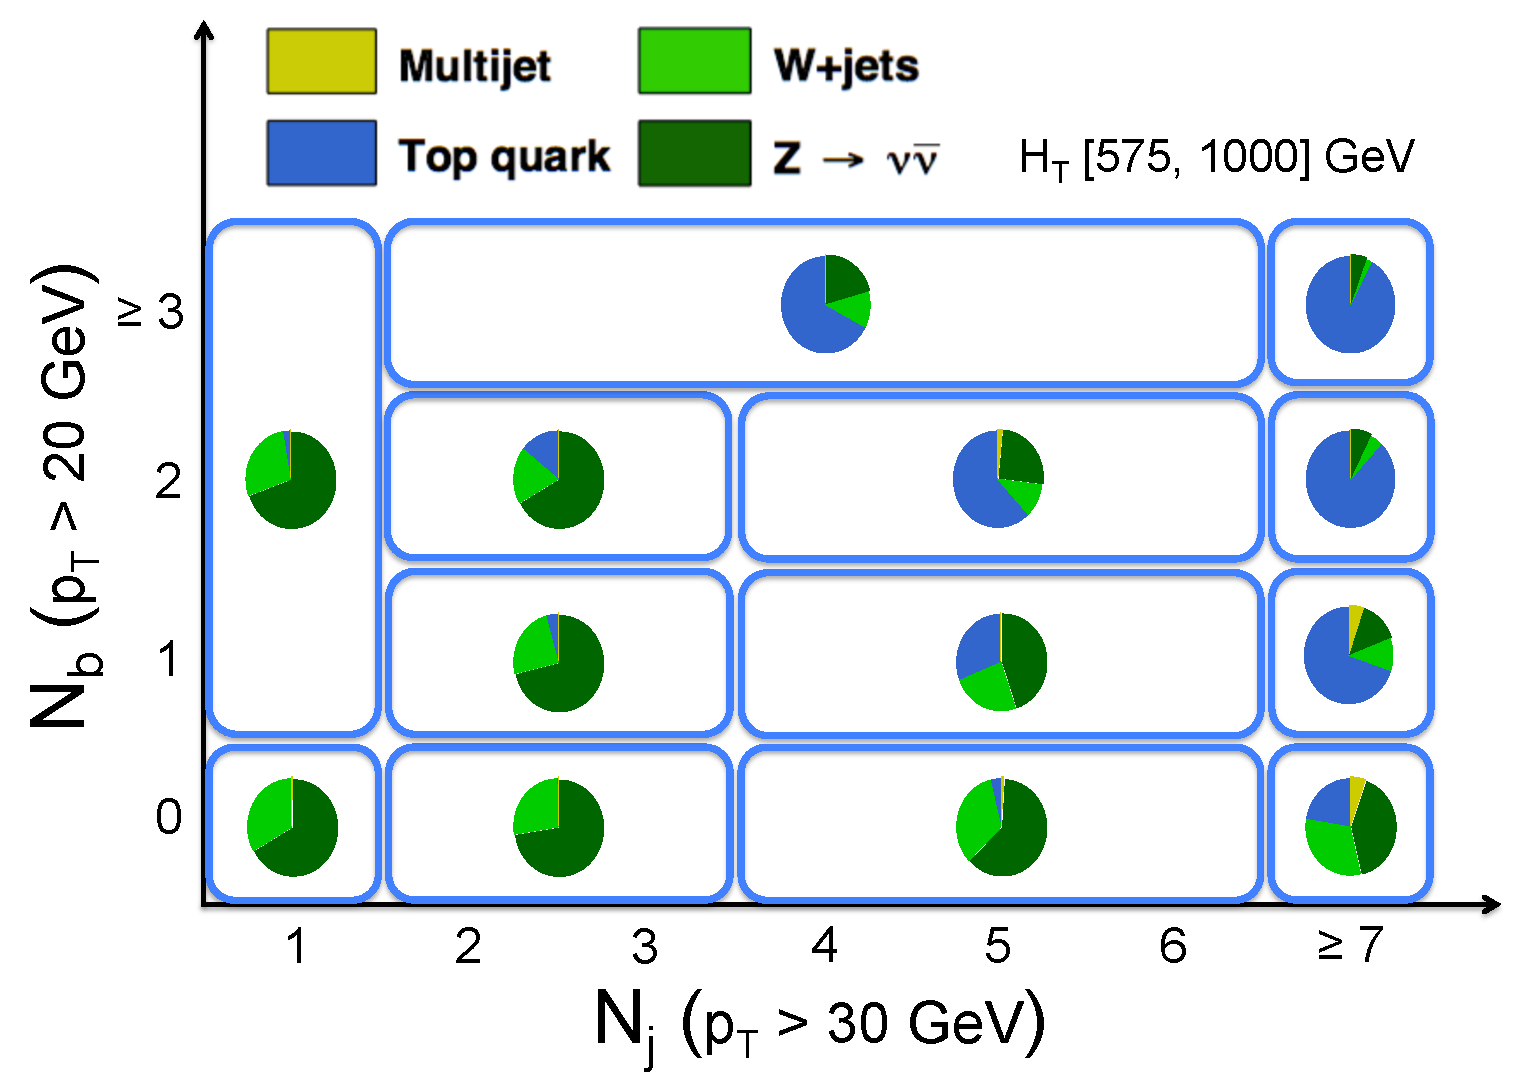
\includegraphics[width=0.75\textwidth]{analysis/figs/bkgComposition_HTlabel}
	\renewcommand{\baselinestretch}{1.0}
	\caption[Topological regions in \nj and \nb for the [575,1000] \HT region.]{Topological regions in \nj and \nb for the [575,1000] \HT region. Within each region, the relative fraction of background events from different SM processes is shown based on simulation.}
	\label{fig:topologicalRegions}
\end{figure}
The different topological regions for one \HT region and their background composition are depicted in figure \ref{fig:topologicalRegions}. Each topological region is further divided into \mttwo bins. The \mttwo binning is constructed such that the low edge of the first bin is 400\GeV in regions with \HT > 1500\GeV and 200\GeV everywhere else, and the low edge of the final bin is constructed to contain approximately one background event based on simulation and not exceeding the maximum \HT value in that topological region (since an upper limit on \HT places an upper limit on \mttwo). The detailed \mttwo binning is as follows:
\begin{itemize}
	\item Very Low \HT: [200,300], [300,400], [400,$\infty$]
	\item Low \HT: [200,300], [300,400], [400,500], [500,$\infty$]
	\item Medium \HT: [200,300], [300,400], [400,600], [600,800], [800,$\infty$]
	\item High \HT: [200,400], [400,600], [600,800], [800, 1000], [1000, 1200], [1200,$\infty$]
	\item Extreme \HT: [400,600], [600,800], [800,1000], [1000,1400], [1400,$\infty$]
\end{itemize}
The various \HT bins and associated \mttwo binning can be seen in figure \ref{fig:mt2bins}, and the full breakdown of signal regions (including \mttwo binning) is listed in tables \ref{tbl:mt2bins1} and \ref{tbl:mt2bins2} .
\begin{figure}
	\centering
	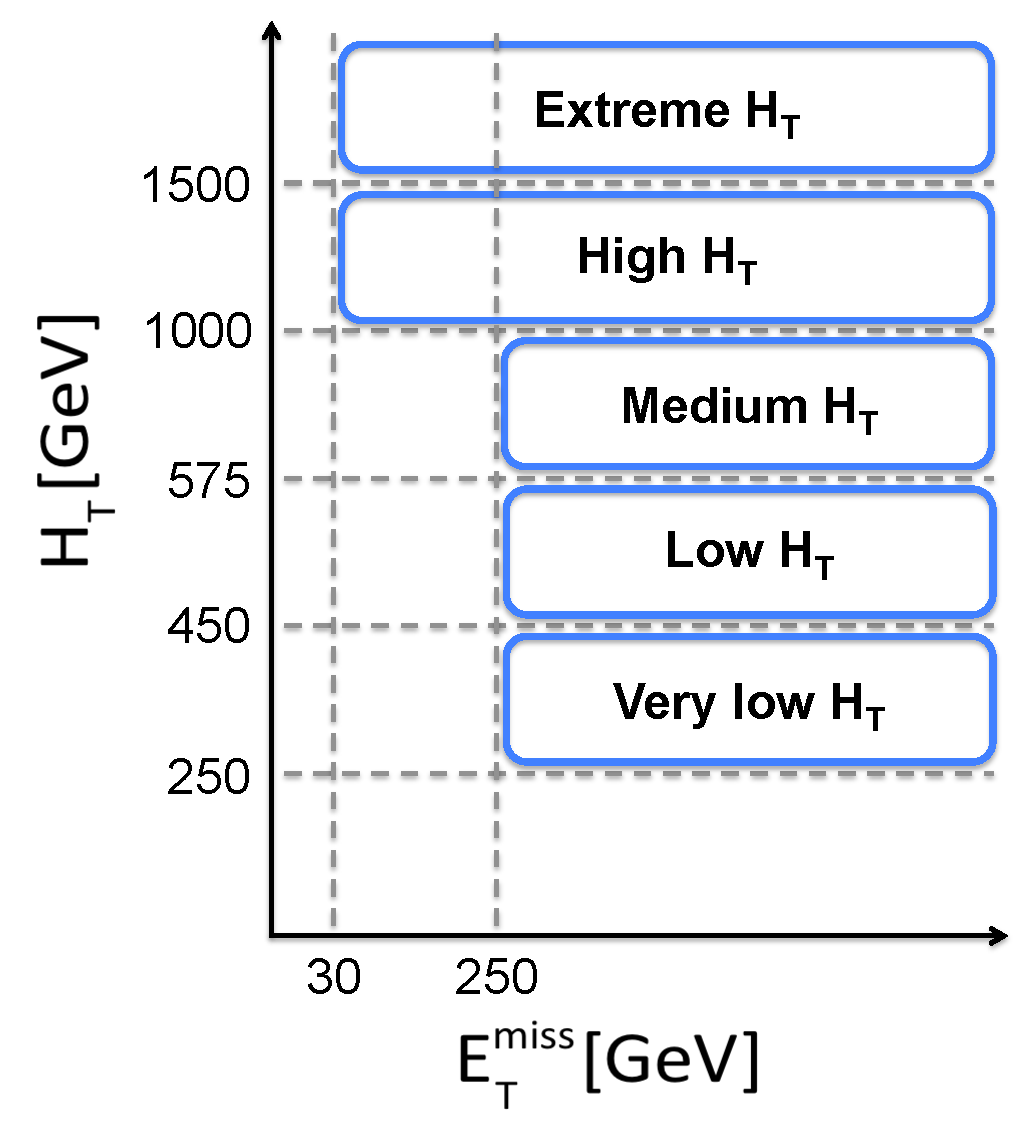
\includegraphics[width=0.38\textwidth]{analysis/figs/HTvsMET_2017}
	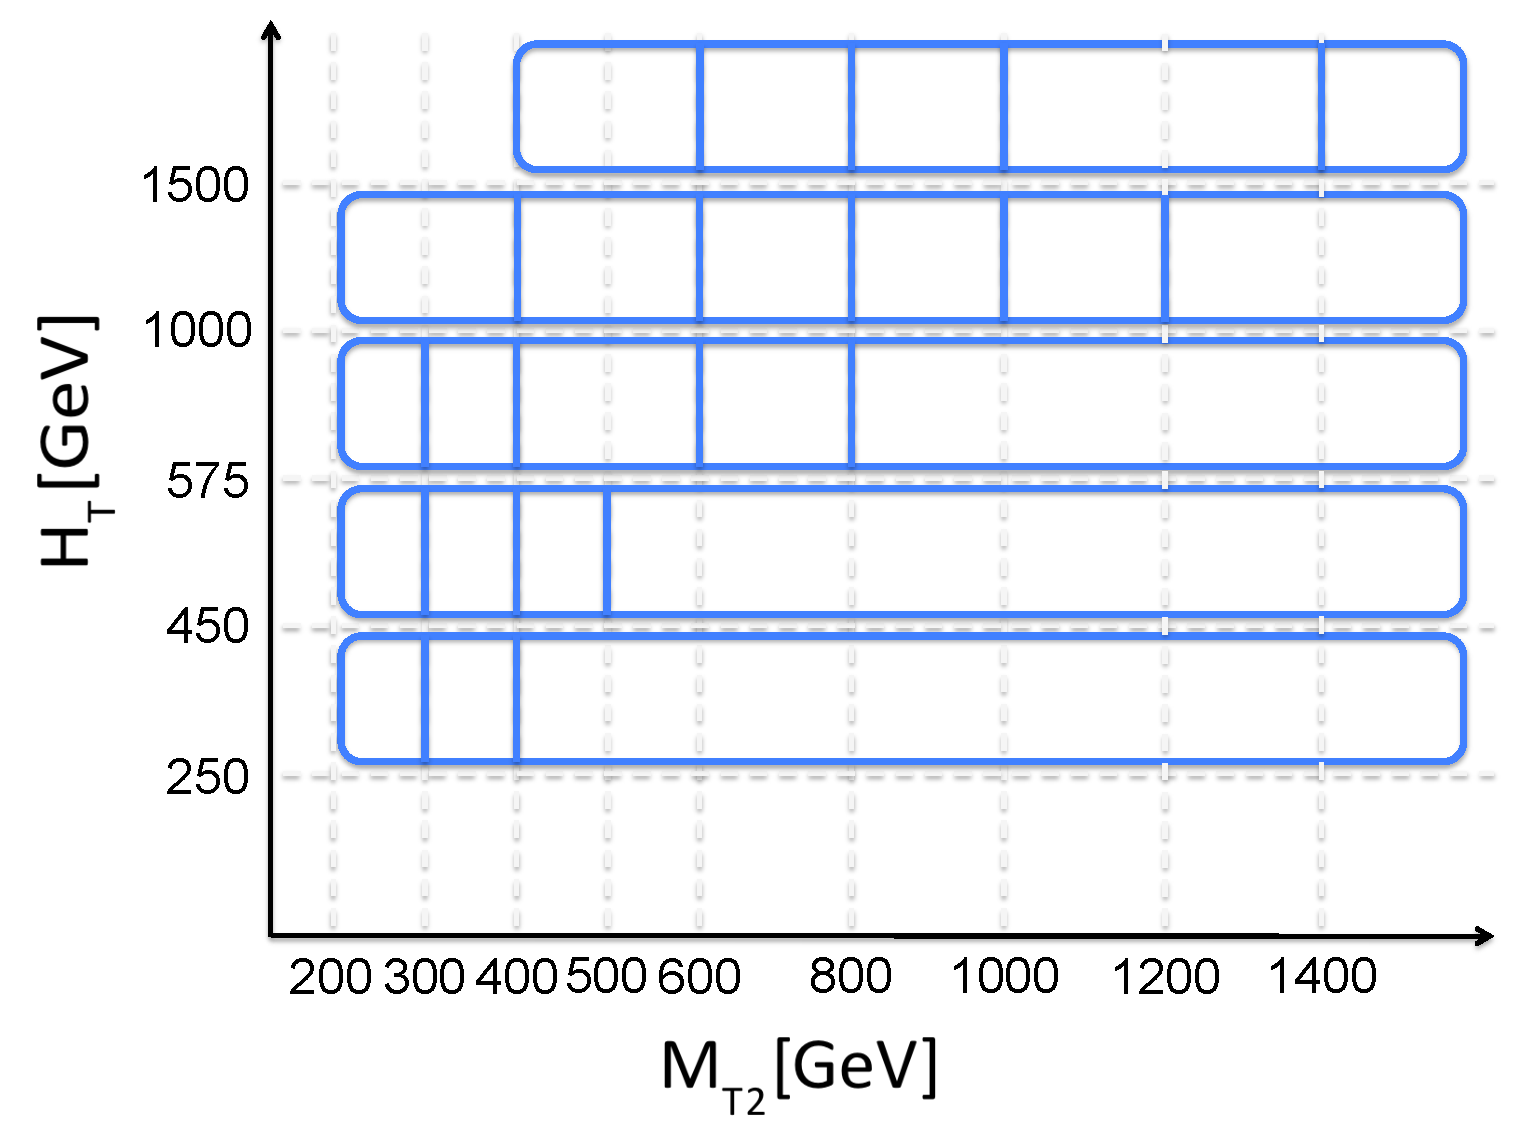
\includegraphics[width=0.55\textwidth]{analysis/figs/HTvsMT2bins_Moriond2017}
	\renewcommand{\baselinestretch}{1.0}
	\caption[Signal region bins in \HT and \MET (left) and \mttwo binning within each \HT region (right).]{Signal region bins in \HT and \MET (left) and \mttwo binning within each \HT region (right). If simulation predicts less than one background event in the greatest \mttwo bin within a region, it is merged with the previous bin.}
	\label{fig:mt2bins}
\end{figure}
\begin{table}[htbp]
	\centering
	\renewcommand{\baselinestretch}{1.0}
	\caption{\mttwo binning in the Very Low, Low, and Medium \HT topological regions.}
	\renewcommand{\arraystretch}{0.65}
	\begin{tabular}{ccl}

\hline

\HT Range [GeV] & Jet Multiplicities & Binning [GeV] \\

\hline%

[ 250, 450 ] & $2-3$j, $  0$b  &  [ 200, 300, 400,  $\infty$ ] \\

 & $2-3$j, $  1$b  &  [ 200, 300, 400,  $\infty$  ] \\

 & $2-3$j, $  2$b  &  [ 200, 300, 400,  $\infty$  ] \\

 & $\geq4$j, $  0$b  &  [ 200, 300, 400,  $\infty$  ] \\

 & $\geq4$j, $  1$b  &  [ 200, 300, 400,  $\infty$  ] \\

 & $\geq4$j, $  2$b  &  [ 200, 300, 400,  $\infty$  ] \\

 & $\geq2$j, $  \geq3$b  &  [ 200, 300, 400,  $\infty$  ] \\ \hline

[ 450, 575 ] & $2-3$j, $  0$b  &  [ 200, 300, 400, 500,  $\infty$  ] \\

 & $2-3$j, $  1$b  &  [ 200, 300, 400, 500,  $\infty$  ] \\

 & $2-3$j, $  2$b  &  [ 200, 300, 400, 500,  $\infty$  ] \\

 & $4-6$j, $  0$b  &  [ 200, 300, 400, 500,  $\infty$  ] \\

 & $4-6$j, $  1$b  &  [ 200, 300, 400, 500,  $\infty$  ] \\

 & $4-6$j, $  2$b  &  [ 200, 300, 400, 500,  $\infty$  ] \\

 & $\geq7$j, $  0$b  &  [ 200, 300, 400,  $\infty$  ] \\

 & $\geq7$j, $  1$b  &  [ 200, 300, 400,  $\infty$  ] \\

 & $\geq7$j, $  2$b  &  [ 200, 300, 400,  $\infty$  ] \\

 & $2-6$j, $  \geq3$b  &  [ 200, 300, 400, 500,  $\infty$  ] \\

 & $\geq7$j, $  \geq3$b  &  [ 200, 300, 400,  $\infty$  ] \\ \hline

[ 575, 1000 ] & $2-3$j, $  0$b  &  [ 200, 300, 400, 600, 800,  $\infty$  ] \\

 & $2-3$j, $  1$b  &  [ 200, 300, 400, 600, 800,  $\infty$  ] \\

 & $2-3$j, $  2$b  &  [ 200, 300, 400, 600, 800,  $\infty$  ] \\

 & $4-6$j, $  0$b  &  [ 200, 300, 400, 600, 800,  $\infty$  ] \\

 & $4-6$j, $  1$b  &  [ 200, 300, 400, 600, 800,  $\infty$  ] \\

 & $4-6$j, $  2$b  &  [ 200, 300, 400, 600, 800,  $\infty$  ] \\

 & $\geq7$j, $  0$b  &  [ 200, 300, 400, 600, 800,  $\infty$  ] \\

 & $\geq7$j, $  1$b  &  [ 200, 300, 400, 600,  $\infty$  ] \\

 & $\geq7$j, $  2$b  &  [ 200, 300, 400, 600,  $\infty$  ] \\

 & $2-6$j, $  \geq3$b  &  [ 200, 300, 400, 600,  $\infty$  ] \\

 & $\geq7$j, $  \geq3$b  &  [ 200, 300, 400, 600,  $\infty$  ] \\ \hline
 
	 \end{tabular}
	\label{tbl:mt2bins1}
\end{table}
\begin{table}
	\centering
	\renewcommand{\baselinestretch}{1.0}
	\caption{\mttwo binning in the High and Extreme \HT topological regions.}
	\renewcommand{\arraystretch}{0.65}
	\begin{tabular}{ccl}

\hline

\HT Range [GeV] & Jet Multiplicities & Binning [GeV] \\

\hline%

[ 1000, 1500 ] & $2-3$j, $  0$b  &  [ 200, 400, 600, 800, 1000, 1200,  $\infty$  ] \\

 & $2-3$j, $  1$b  &  [ 200, 400, 600, 800, 1000, 1200,  $\infty$  ] \\

 & $2-3$j, $  2$b  &  [ 200, 400, 600, 800, 1000,  $\infty$  ] \\

 & $4-6$j, $  0$b  &  [ 200, 400, 600, 800, 1000, 1200,  $\infty$  ] \\

 & $4-6$j, $  1$b  &  [ 200, 400, 600, 800, 1000, 1200,  $\infty$  ] \\

 & $4-6$j, $  2$b  &  [ 200, 400, 600, 800, 1000,  $\infty$  ] \\

 & $\geq7$j, $  0$b  &  [ 200, 400, 600, 800, 1000,  $\infty$  ] \\

 & $\geq7$j, $  1$b  &  [ 200, 400, 600, 800,  $\infty$  ] \\

 & $\geq7$j, $  2$b  &  [ 200, 400, 600, 800,  $\infty$  ] \\

 & $2-6$j, $  \geq3$b  &  [ 200, 400, 600,  $\infty$  ] \\

 & $\geq7$j, $  \geq3$b  &  [ 200, 400, 600,  $\infty$  ] \\ \hline

[ 1500, $\infty$  ] & $2-3$j, $  0$b  &  [ 400, 600, 800, 1000, 1400,  $\infty$  ] \\

 & $2-3$j, $  1$b  &  [ 400, 600, 800, 1000,  $\infty$  ] \\

 & $2-3$j, $  2$b  &  [ 400,  $\infty$  ] \\

 & $4-6$j, $  0$b  &  [ 400, 600, 800, 1000, 1400,  $\infty$  ] \\

 & $4-6$j, $  1$b  &  [ 400, 600, 800, 1000, 1400,  $\infty$  ] \\

 & $4-6$j, $  2$b  &  [ 400, 600, 800,  $\infty$  ] \\

 & $\geq7$j, $  0$b  &  [ 400, 600, 800, 1000,  $\infty$  ] \\

 & $\geq7$j, $  1$b  &  [ 400, 600, 800,  $\infty$  ] \\

 & $\geq7$j, $  2$b  &  [ 400, 600, 800,  $\infty$  ] \\

 & $2-6$j, $  \geq3$b  &  [ 400, 600, $\infty$  ] \\

 & $\geq7$j, $  \geq3$b  &  [ 400, $\infty$ ] \\ 

\hline
	\end{tabular}
	\label{tbl:mt2bins2}
\end{table}
In addition to multijet search regions, this analysis also considers monojet events. Because there is only a single jet (and \mttwo is ill-defined without multiple jets), binning in these regions is defined using \nb and \HT as follows:
\begin{itemize}
	\item \nb: 0b, $\geq$1b
	\item \HT: [250,350], [350,450], [450,575], [575,700], [700,1000], [1000,1200], [1200,$\infty$]
\end{itemize}
As with the multijet regions, monojet \HT bins with less than one simulated background event in the final bin are merged with the penultimate bin.

In addition to these signal regions used to interpret results in the context of various BSM physics models, the analysis also provides results in "super signal regions" (SSRs) as defined in table \ref{tbl:ssr}. These regions provide a simpler set of selections than the nominal signal regions so that phenomenologists may easily reinterpret results in the context of different signal models. Results obtained using the SSRs are not as sensitive as the nominal binning --- finely binned regions have a higher signal-to-background ratio and the global background fit reduces the background uncertainties --- but are much easier to use for reinterpretation than the many correlated bins of the full analysis.
\begin{table}
	\centering
	\renewcommand{\baselinestretch}{1.0}
	\caption{Definition of "super signal regions" used in reinterpretations of the analysis.}
	\begin{tabular}{l||c|c|c|c}
\hline\hline
Region & \nj & \nb & \HT [GeV] & \mttwo [GeV] \\
\hline\hline
2j loose & $\geq 2$ & - & $> 1000$ & $> 1200$ \\
2j tight & $\geq 2$ & - & $> 1500$ & $> 1400$ \\
\hline
4j loose & $\geq 4$ & - & $> 1000$ & $> 1000$ \\
4j tight & $\geq 4$ & - & $> 1500$ & $> 1400$ \\
\hline
7j loose & $\geq 7$ & - & $> 1000$ & $> 600$ \\
7j tight & $\geq 7$ & - & $> 1500$ & $> 800$ \\
\hline
2b loose & $\geq 2$ & $\geq 2$ & $> 1000$ & $> 600$ \\
2b tight & $\geq 2$ & $\geq 2$ & $> 1500$ & $> 600$ \\
\hline
3b loose & $\geq 2$ & $\geq 3$ & $> 1000$ & $> 400$ \\
3b tight & $\geq 2$ & $\geq 3$ & $> 1500$ & $> 400$ \\
\hline
7j3b loose & $\geq 7$ & $\geq 3$ & $> 1000$ & $> 400$ \\
7j3b tight & $\geq 7$ & $\geq 3$ & $> 1500$ & $> 400$ \\
\hline
	\end{tabular}
	\label{tbl:ssr}
\end{table}

\section{Control Regions}
\label{sec:controlRegions}
In order to anchor the data-driven background estimates used in this analysis, {\it control regions} (CR) orthogonal to the signal region selection are defined for various processes. In particular, there are control regions corresponding to enriched samples of single lepton events, \zll events, and QCD multijet events.
%
%\subsection{$\gamma$ + jet Control Region}
%\label{subsec:gammaCR}
%
%\fm{photon plus jets CR selection}

\subsection{Single Lepton Control Region}
\label{subsec:leptonCR}
The single lepton CR is constructed to select a sample enriched with single lepton events, the most dominant contributions being from \ttbar and \wjets production. The same baseline selections described in section \ref{sec:eventSelection} are applied with the exception of the following:
\begin{itemize}
	\item In lieu of the lepton veto, exactly one lepton candidate passing the reco or PF lepton selections is required. In order to avoid double counting (for leptons which are reconstructed both as a reco lepton and PF candidate), PF leptons within \DR < 0.1 of a reco lepton are not considered. 
	\item The transverse mass \MT between the lepton and \MET must be less than 100\GeV to reduce possible signal contamination.
\end{itemize}
Since non-isolated leptons in the fiducial region of the detector are usually successfully reconstructed, the closest jet within \DR < 0.4 of the lepton is removed and the lepton instead counted as a visible object for the purposes of computing \Ht, \Htmiss, \dphilong, \htovermet, and \mttwo (as well as the hemispheres used to calculate \mttwo). Events are further subdivided into the topological regions described in section \ref{sec:searchRegions} using the modified \HT and \nj and \nb, but not in \mttwo to increase the statistical power of the CR. The signal regions with $\geq7$j,$\geq1$b are all predicted using CRs with identical \Ht bins but $\geq7$j,1-2b to increase the statistical power of those CRs (and to avoid signal contamination in regions with $\geq7$j,$\geq3$b). In addition, for regions with $\HT > 1500\GeV$, the minimum \mttwo threshold is set to 200\GeV to increase available statistics. The monojet CR is binned identically to the signal region.

\subsection{Dilepton Control Region}
\label{subsec:zllCR}

Control regions corresponding to opposite-sign same-flavor leptons (OSSF) from \zll events are used to estimate the \znunu background, with corresponding sets of control regions requiring an opposite-sign opposite-flavor (OSOF) pair to estimate the flavor-symmetric background component in the former dilepton CR. The same baseline selections as described in section \ref{sec:eventSelection} are applied with the exception of the follow:
\begin{itemize}
	\item In lieu of the lepton veto, exactly 2 leptons ($ee$, $e\mu$, or $\mu\mu$) passing loose lepton selections are required.
	\item There is no requirement on \MET. Instead, the dilepton system must have a transverse momentum $p_{\mathrm{T}}(\ell\ell) > 200\GeV$ to mimic the kinematics of the \znunu background and suppress the \ttbar contribution.
	\item Without a missing energy requirement, events are selected in data using leptonic trigger paths. Dimuon events are selected using a combination of dimuon and high-\pt single muon triggers, dielectron events using a combination of dielectron and high-\pt single photon paths (which do not require isolation and recover efficiency for high-\pt electrons or those highly co-linear high-\pt Z bosons), and opposite-flavor events are selected using a combination of $e\mu$ triggers and higher threshold single-lepton paths (to again recover efficiency for some events).
	\item To improve trigger efficiency for these regions, the leading lepton is required to have a minimum momentum $\pt > 100\GeV$ and the sub-leading lepton $\pt > 30\GeV$.
	\item When selecting Z boson candidates for the \znunu estimate, the leptons are also required to be OSSF with an invariant mass $|\mll - m_{\mathrm{Z}}| < 20\GeV$, where $m_{\mathrm{Z}}$ is the nominal Z boson mass.
\end{itemize}
Similar to the single lepton control region, the closest jet within \DR < 0.4 of each lepton is removed and the leptons added to the \MET vector for the purposes of computing \nj, \nb, \Ht, \Htmiss, \dphilong, \htovermet, and \mttwo (as well as the hemispheres used to calculate \mttwo). Additional information on the \mttwo binning for these regions is detailed in section \ref{sec:zinv}.

\subsection{Multijet Control Region}
\label{subsec:multijetCR}

The multijet control region is designed to select  a sample enriched in QCD events to estimate the multijet background. The same baseline selections described in section \ref{sec:eventSelection} are applied with the exception of the \dphilong requirement, which is inverted to select a sample dominated by QCD events with large fake \MET due to jet energy mismeasurements.

The transfer factor which is used to extrapolate the control region yield to the signal region is measured in a separate QCD-dominated region with $\mttwomath < 200\GeV$, described in detail in section \ref{sec:qcd}. Because of the lower \MET requirement, different trigger paths must be used. For regions with $\HT > 1000\GeV$, trigger paths seeded by a single high-\pt jet are used. For other \HT regions, similar trigger paths with lower jet \pt thresholds are used, but due to the rate of QCD events creating low-\pt jets these paths are prescaled to suppress the data acquisition rate.

This chapter makes use of figures and tables from the \mttwo paper and internal analysis note to illustrate the analysis design, methodology, and results. This work was made possible by contributions from the rest of the Surf \& Turf group, our collaborators at ETH Zurich, and the many other CMS members in the SUSY group and beyond.

% --------------------------------------------------------------------------- %
% --------------------------------------------------------------------------- %

% --------------------------------------------------------------------------- %
% --------------------------------------------------------------------------- %
\chapter{Background Estimates}
\label{ch:bkgs}

\section{Types of Backgrounds}
\label{sec:bkgs}

\section{Multi-jet Estimate}
\label{sec:qcd}

\section{Lost Lepton Estimate}
\label{sec:lostlep}

\section{Invisible Z Estimate}
\label{sec:zinv}
% --------------------------------------------------------------------------- %
% --------------------------------------------------------------------------- %

% --------------------------------------------------------------------------- %
% --------------------------------------------------------------------------- %
\chapter{Results}
\label{ch:results}
The techniques described in this analysis are applied to 35.9\fbinv of proton-proton collision data gathered at the LHC and recorded by the CMS detector. Observed yields in each signal region are further interpreted in the context of simplified SUSY models to establish new limits on the masses of hypothesized BSM particles.

% --------------------------------------------------------------------------- %
% --------------------------------------------------------------------------- %
\section{Yields and Background Fits}
\label{sec:yields}

The observed yield in the search regions is statistically compatible with the predicted background from SM processes. A summary of the total yield in each signal region and predicted background contribution relying only on the techniques described in chapter \ref{ch:bkgs}, referred to as {\it pre-fit} results, is illustrated for each topological region in figure \ref{fig:yieldPrefitTopological}, and the individual yield in each \mttwo bin can be found in figures \ref{fig:yieldPrefit1}, \ref{fig:yieldPrefit2}, and \ref{fig:yieldPrefit3}.
\begin{figure}
	\centering
	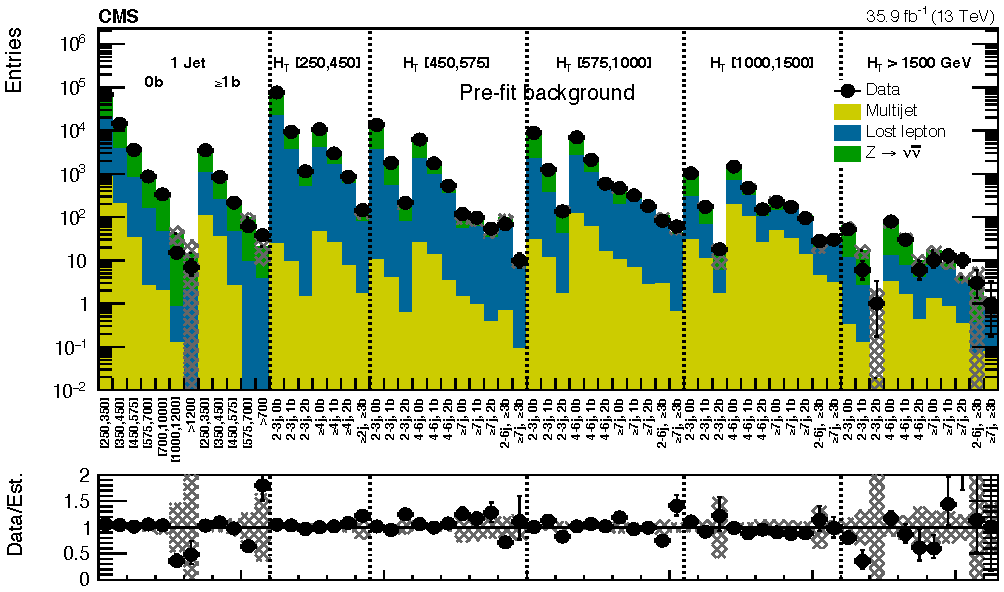
\includegraphics[width=0.95\textwidth]{results/figs/mt2_ALL_fullEstimate}
	\renewcommand{\baselinestretch}{1.0}
	\caption[The data yield in each topological region compared to the pre-fit background prediction.]{The data yield in each topological region compared to the pre-fit background prediction. The hatched bands illustrate the total uncertainty in the background estimate. Results in the monojet regions are binned in jet \pt, while those in the multijet regions are labeled according to \nj and \nb.}
	\label{fig:yieldPrefitTopological}
\end{figure}
\begin{figure}
	\centering
	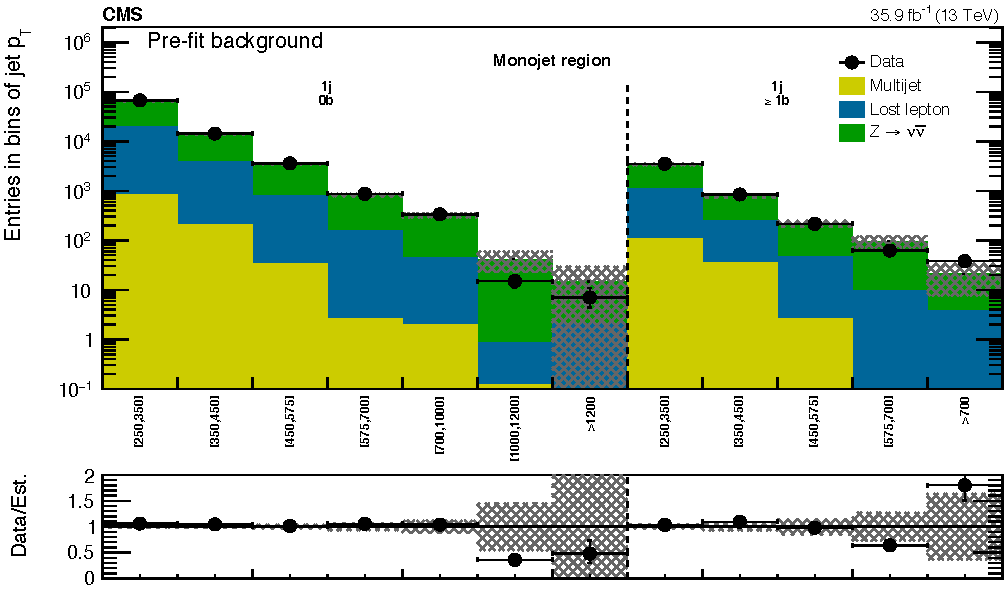
\includegraphics[width=0.90\textwidth]{results/figs/mt2_monojet_fullEstimate}
	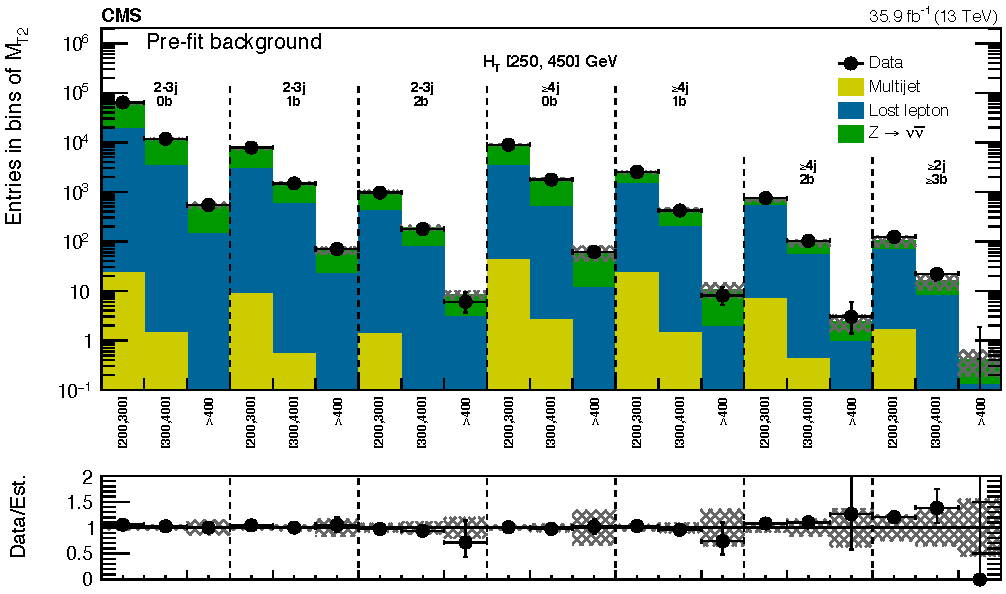
\includegraphics[width=0.90\textwidth]{results/figs/mt2_veryLowHT_fullEstimate}
	\renewcommand{\baselinestretch}{1.0}
	\caption[The data yield in the monojet and very-low \HT regions compared to the pre-fit background prediction.]{The data yield in the monojet and very-low \HT regions compared to the pre-fit background prediction. The hatched bands illustrate the total uncertainty in the background estimate. Results in the monojet regions are binned in jet \pt in units of GeV, while those in the multijet regions are labeled according to \mttwo bin in units of GeV.}
	\label{fig:yieldPrefit1}
\end{figure}
\begin{figure}
	\centering
	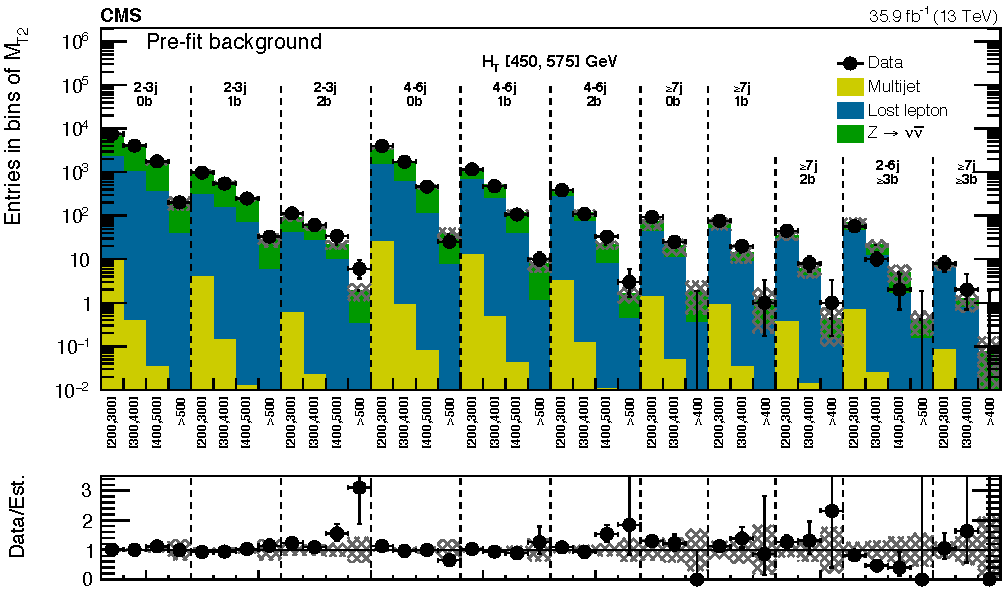
\includegraphics[width=0.90\textwidth]{results/figs/mt2_lowHT_fullEstimate}
	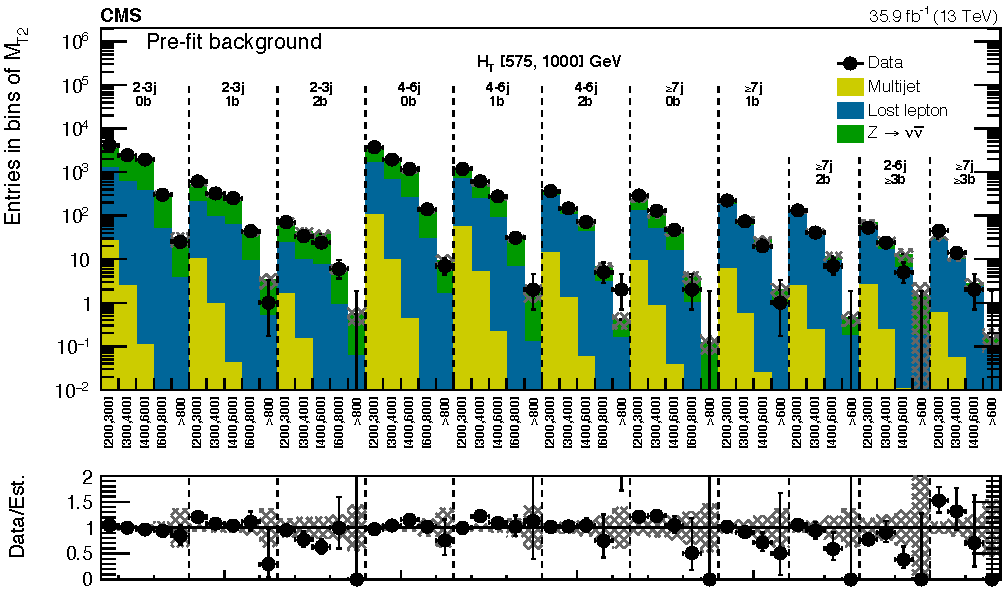
\includegraphics[width=0.90\textwidth]{results/figs/mt2_mediumHT_fullEstimate}
	\renewcommand{\baselinestretch}{1.0}
	\caption[The data yield in the low \HT and medium \HT regions compared to the pre-fit background prediction.]{The data yield in the low \HT and medium \HT regions compared to the pre-fit background prediction. The hatched bands illustrate the total uncertainty in the background estimate. Results are labeled according to \mttwo bin in units of GeV.}
	\label{fig:yieldPrefit2}
\end{figure}
\begin{figure}
	\centering
	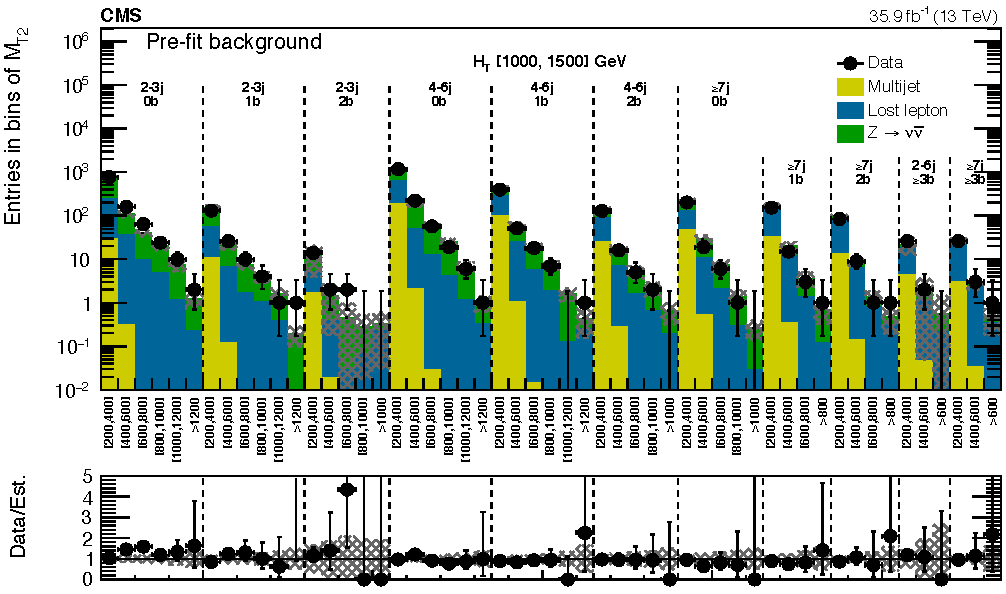
\includegraphics[width=0.90\textwidth]{results/figs/mt2_highHT_fullEstimate}
	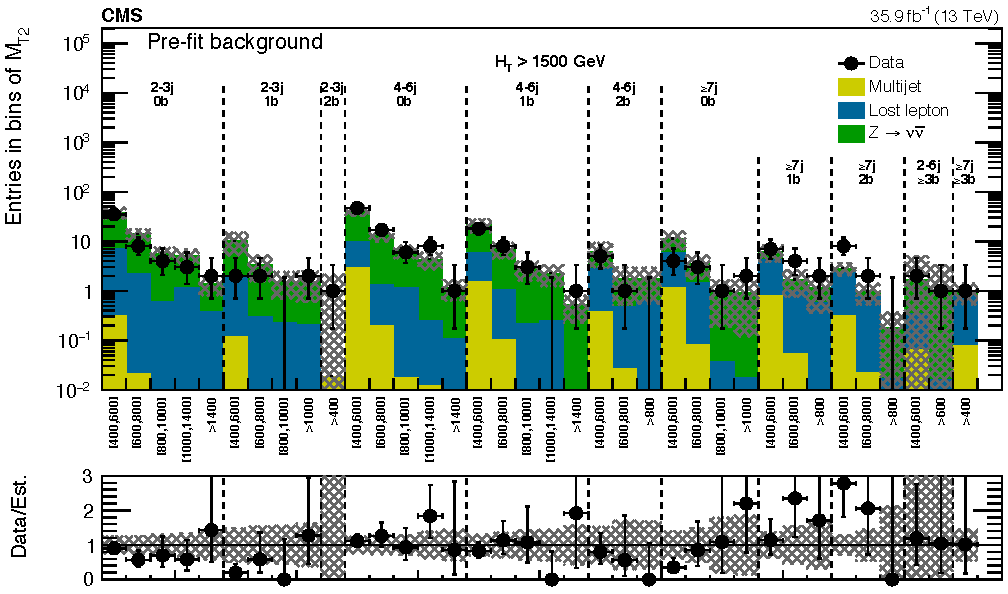
\includegraphics[width=0.90\textwidth]{results/figs/mt2_extremeHT_fullEstimate}
	\renewcommand{\baselinestretch}{1.0}
	\caption[The data yield in the high \HT and extreme \HT regions compared to the pre-fit background prediction.]{The data yield in the high \HT and extreme \HT regions compared to the pre-fit background prediction. The hatched bands illustrate the total uncertainty in the background estimate. Results are labeled according to \mttwo bin in units of GeV.}
	\label{fig:yieldPrefit3}
\end{figure}

The background estimate is further refined by performing a maximum-likelihood fit to data in each signal region, referred to as {\it post-fit} results. The fit is performed using both background-only or background-plus-signal hypotheses to set limits on simplified physics models described in section \ref{sec:interpretations}. The estimates and uncertainties on each background as described in chapter \ref{ch:bkgs} are  used as inputs to the fitting procedure, where the likelihood is constructed as a product of Poisson probability density functions for each signal region with constraints set according to the background uncertainties and signal uncertainties (described in section \ref{subsec:signalSyst}). The post-fit yield for each topological region is illustrated in figure \ref{fig:yieldPostfitTopological}, and the individual yield in each \mttwo bin can be found in figures \ref{fig:yieldPostfit1}, \ref{fig:yieldPostfit2}, and \ref{fig:yieldPostfit3}. The post-fit procedure has the effect of constraining background and its associated uncertainties when the fitting procedure is applied to data consistent with predictions modeling uncertainties appropriately.
\begin{figure}
	\centering
	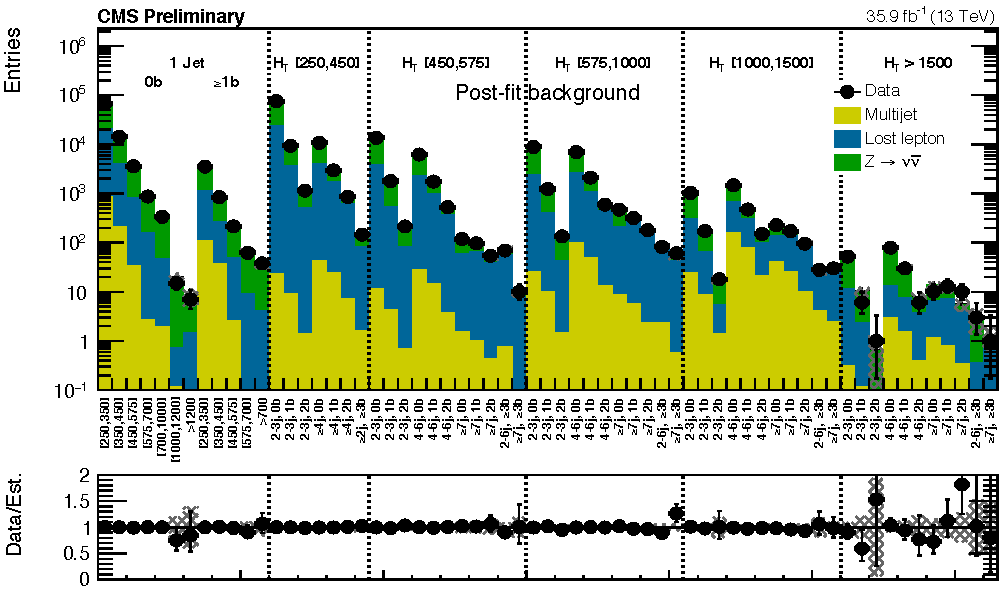
\includegraphics[width=0.90\textwidth]{results/figs/postfit/mt2_ALL_fullEstimate}
	\renewcommand{\baselinestretch}{1.0}
	\caption[The data yield in each topological region compared to the post-fit background prediction.]{The data yield in each topological region compared to the post-fit background prediction. The hatched bands illustrate the total uncertainty in the background estimate. Results in the monojet regions are binned in jet \pt, while those in the multijet regions are labeled according to \nj and \nb.}
	\label{fig:yieldPostfitTopological}
\end{figure}
\begin{figure}
	\centering
	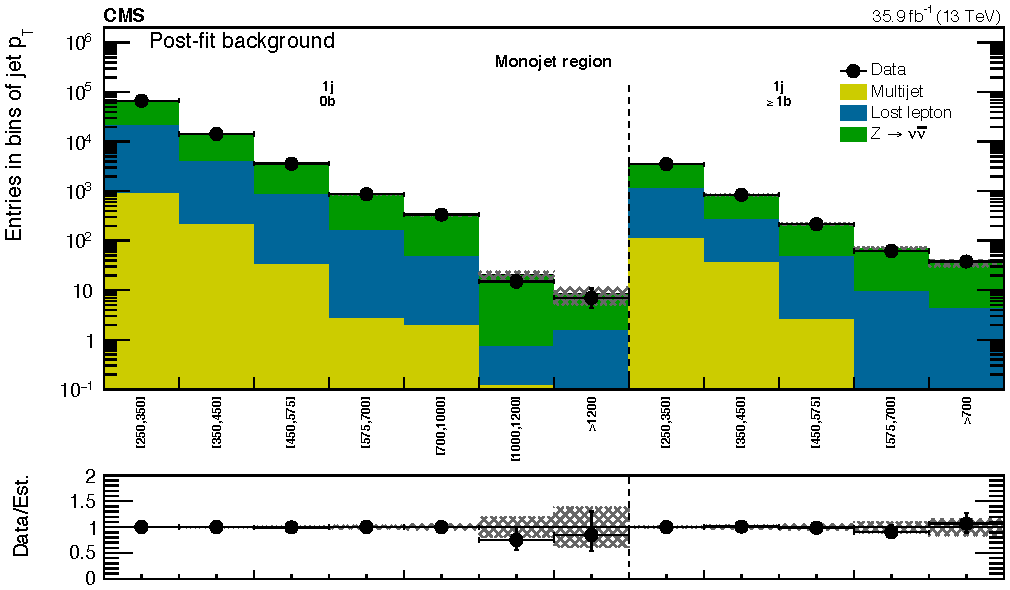
\includegraphics[width=0.90\textwidth]{results/figs/postfit/mt2_monojet_fullEstimate}
	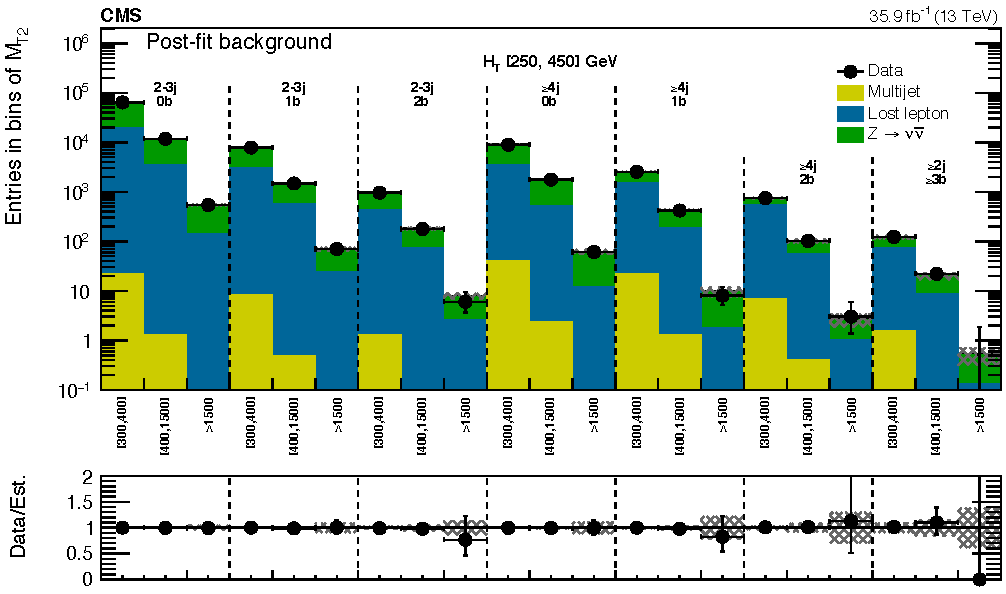
\includegraphics[width=0.90\textwidth]{results/figs/postfit/mt2_veryLowHT_fullEstimate}
	\renewcommand{\baselinestretch}{1.0}
	\caption[The data yield in the monojet and very-low \HT regions compared to the post-fit background prediction.]{The data yield in the monojet and very-low \HT regions compared to the post-fit background prediction. The hatched bands illustrate the total uncertainty in the background estimate. Results in the monojet regions are binned in jet \pt in units of GeV, while those in the multijet regions are labeled according to \mttwo bin in units of GeV.}
	\label{fig:yieldPostfit1}
\end{figure}
\begin{figure}
	\centering
	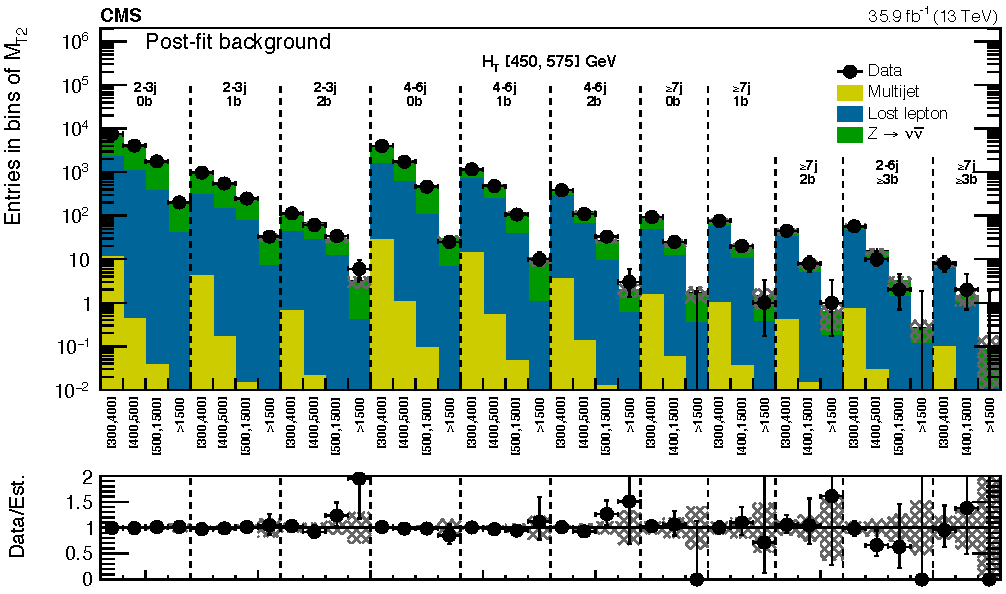
\includegraphics[width=0.90\textwidth]{results/figs/postfit/mt2_lowHT_fullEstimate}
	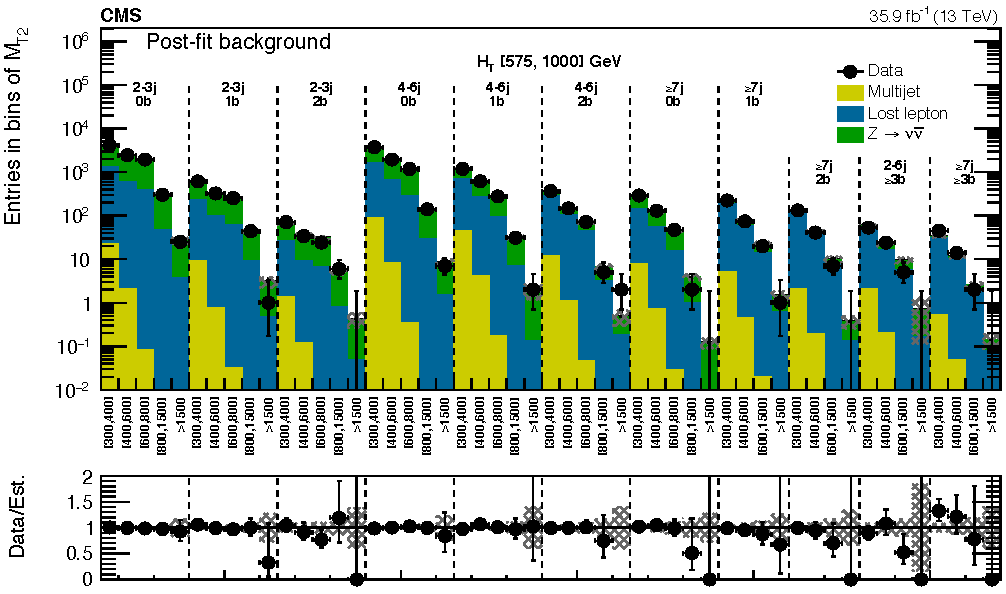
\includegraphics[width=0.95\textwidth]{results/figs/postfit/mt2_mediumHT_fullEstimate}
	\renewcommand{\baselinestretch}{1.0}
	\caption[The data yield in the low \HT and medium \HT regions compared to the post-fit background prediction.]{The data yield in the low \HT and medium \HT regions compared to the post-fit background prediction. The hatched bands illustrate the total uncertainty in the background estimate. Results are labeled according to \mttwo bin in units of GeV.}
	\label{fig:yieldPostfit2}
\end{figure}
\begin{figure}
	\centering
	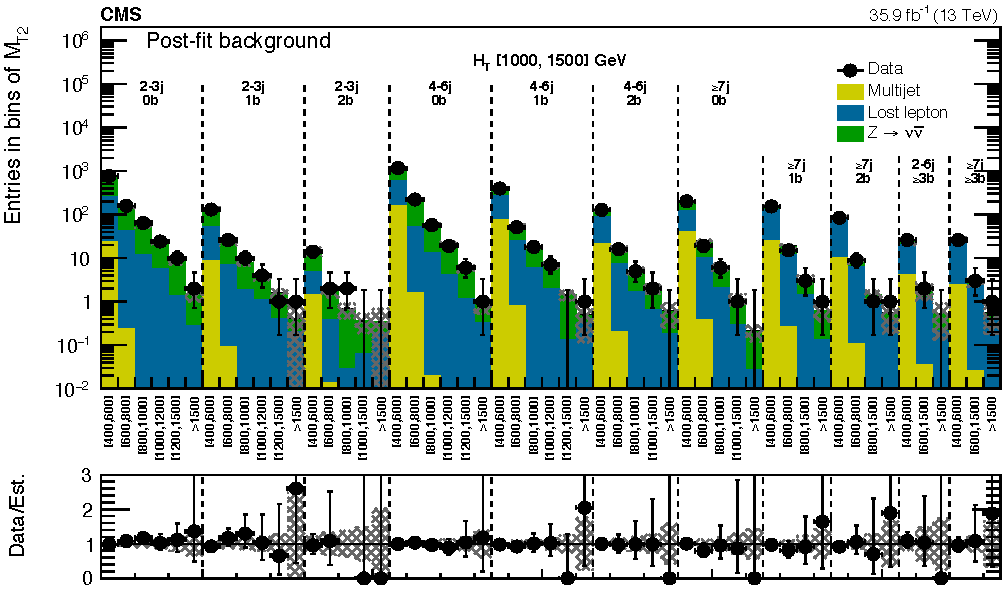
\includegraphics[width=0.90\textwidth]{results/figs/postfit/mt2_highHT_fullEstimate}
	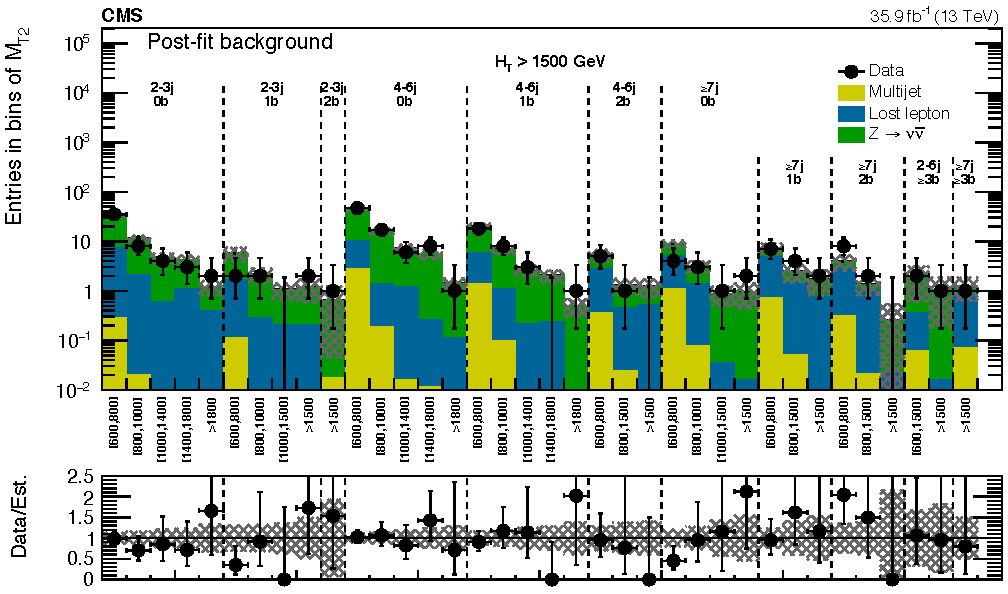
\includegraphics[width=0.90\textwidth]{results/figs/postfit/mt2_extremeHT_fullEstimate}
	\renewcommand{\baselinestretch}{1.0}
	\caption[The data yield in the high \HT and extreme \HT regions compared to the post-fit background prediction.]{The data yield in the high \HT and extreme \HT regions compared to the post-fit background prediction. The hatched bands illustrate the total uncertainty in the background estimate. Results are labeled according to \mttwo bin in units of GeV.}
	\label{fig:yieldPostfit3}
\end{figure}
% --------------------------------------------------------------------------- %
% --------------------------------------------------------------------------- %

% --------------------------------------------------------------------------- %
% --------------------------------------------------------------------------- %
\section{Signal Interpretations}
\label{sec:interpretations}

The results of the search can be interpreted as a constraint on the mass of hypothesized particles of various BSM models. Based on the simulated production processes of simplified SUSY models, this section describes some of the uncertainties associated with the signal yield, as well as the limits associated with various simplified models of interest.

\subsection{Signal Yield Systematic Uncertainties}
\label{subsec:signalSyst}

The uncertainties associated with the signal yield are summarized in table \ref{tbl:signalSyst}. The various sources of uncertainty are described in detail below:
\begin{itemize}
	\item {\it Luminosity:} the uncertainty of the total integrated luminosity delivered by the LHC is evaluated in {\it Van Der Meer scans}, where the rate of interactions is measured while scanning the colliding proton beams across each other. The uncertainty in the luminosity based on these studies is 2.5\%.
	\item {\it Simulation statistics:} the limited size of the Monte Carlo samples for each sample effect the statistics in each signal region bin. After applying the signal selection, the statistical uncertainty can range from 1-100\% in different bins, though bins with large uncertainty typically correspond to those with low signal acceptance, and thus do not drive the sensitivity of the analysis to that simplified model mass point.
	\item {\it Renormalization and factorization scales:} the overall effect of varying the simulation renormalization and factorization scales of the underlying physics processes (and subsequent effect on event kinematics) is computed separately in each bin. The result of this variation is relatively flat and minor across the signal bins, and is conservatively estimated at 5\% for all regions.
	\item {\it Initial-state radiation (ISR) recoil:} variations of the boost due to initial-state radiation are performed to test the modeling of ISR effects in simulation. The effect of these variations ranges from 0-30\% across signal regions.
	\item {\it b-tagging efficiency:} the effect of varying the b-tag scale factor efficiency is calculated in each bin, and taken as a correlated error amongst all bins. The effect of this variation for heavy (light) flavor jets is 0-40\% (0-20\%) across signal regions.
	\item {\it Lepton efficiency:} the effect of varying the electron and muon scale factors applied to simulation is calculated in each bin, and taken as a correlated error amongst all bins. The effect of this variation is 0-20\% across signal regions.
	\item {\it Jet energy scale:} the effect of varying the jet energy scales is calculated in each bin, and the results are compatible with statistical uncertainty for low-statistics bins. Based on findings in the high-statistics bins, the uncertainty is estimated at 5\% for all regions.
	\item {\it Fast simulation modeling:} The signal Monte Carlo samples are generated using the FastSim package, which may result in modeling differences compared to Fullsim MC. Studies of the Fastsim kinematics with respect to \MET and pile-up modeling indicate differences of up to 5\% in some signal regions.
\end{itemize}

\begin{table}
	\centering
	\begin{tabular}{l|c|c}
\hline
Source & Typical Values & Correlated? \\
\hline
Luminosity                                & 2.6\%     & \checkmark\\
Limited size of MC samples                & 1--100\%  & - \\
Renormalization and factorization scales  & 5\%       & - \\
%Parton distribution functions             & 10\%      \\
``ISR'' recoil                            & 0--30\%   & \checkmark\\
B-tagging efficiency, heavy flavor        & 0--40\%   & \checkmark\\
B-tagging efficiency, light flavor        & 0--20\%   & \checkmark\\
Lepton efficiency                         & 0--20\%   & \checkmark\\
Jet energy scale                          & 5\%       & - \\
Fast simulation \MET\ modeling            & 0-5\%     & \checkmark\\
Fast simulation pileup modeling           & 4.6\%     & \checkmark\\
%%%Luminosity                                & 2.6\%    & \checkmark \\
%%%MC statistics                             & 1--100\% & - \\
%%%Renormalization and factorization scales  & 5\%      & - \\
%%%``ISR'' recoil                            & 0--30\%  & \checkmark \\
%%%B-tagging efficiency, heavy flavor        & 0--40\%  & \checkmark \\
%%%B-tagging efficiency, light flavor        & 0--20\%  & \checkmark \\
%%%Lepton efficiency (models with leptons only)           & 0--20\%  & \checkmark \\
%%%Jet energy scale                          & 5\%      & - \\
%%%Generator \MET systematic                 & 0-5\%    & \checkmark \\
\hline
\end{tabular}
	\caption{Typical values of the systematic uncertainties associated with the simplified SUSY model signal yield for each interpretation in this search. Some systematics are taken as correlated amongst all signal regions; the rest are uncorrelated everywhere. Note that the large range of statistical uncertainty is driven by a small number of signal regions with low acceptance (which are not typically sensitive to those model points).}
	\label{tbl:signalSyst}
\end{table}

\subsection{Exclusion Limits}
\label{subsec:exclusionLimits}

The final results are interpreted in the context of various simplified SUSY models: gluino-mediated squark pair production, direct production of squarks, and alternative models of top squark production with different decay modes. Each of these models is illustrated in figure \ref{fig:signalFeynman}. For each pair producing gluino (squark) scenario, the models assume all SUSY particles other than the gluino (squark) and lightest neutralino are too massive to be produced directly and the gluino (squark) decays promptly. In addition, each model assumes that the gluino (squark) decays with a 100\% branching fraction into the decay products depicted in figure \ref{fig:signalFeynman}, except for models where the decays of the two squarks differ where a 50\% branching fraction for each decay mode is assumed. When considering top squark pair production, the polarization of the top quark is model dependent (and a function of the top-squark and neutralino mixing matrices), so events are generated without polarization to remain model-independent.
\begin{figure}
	\centering
	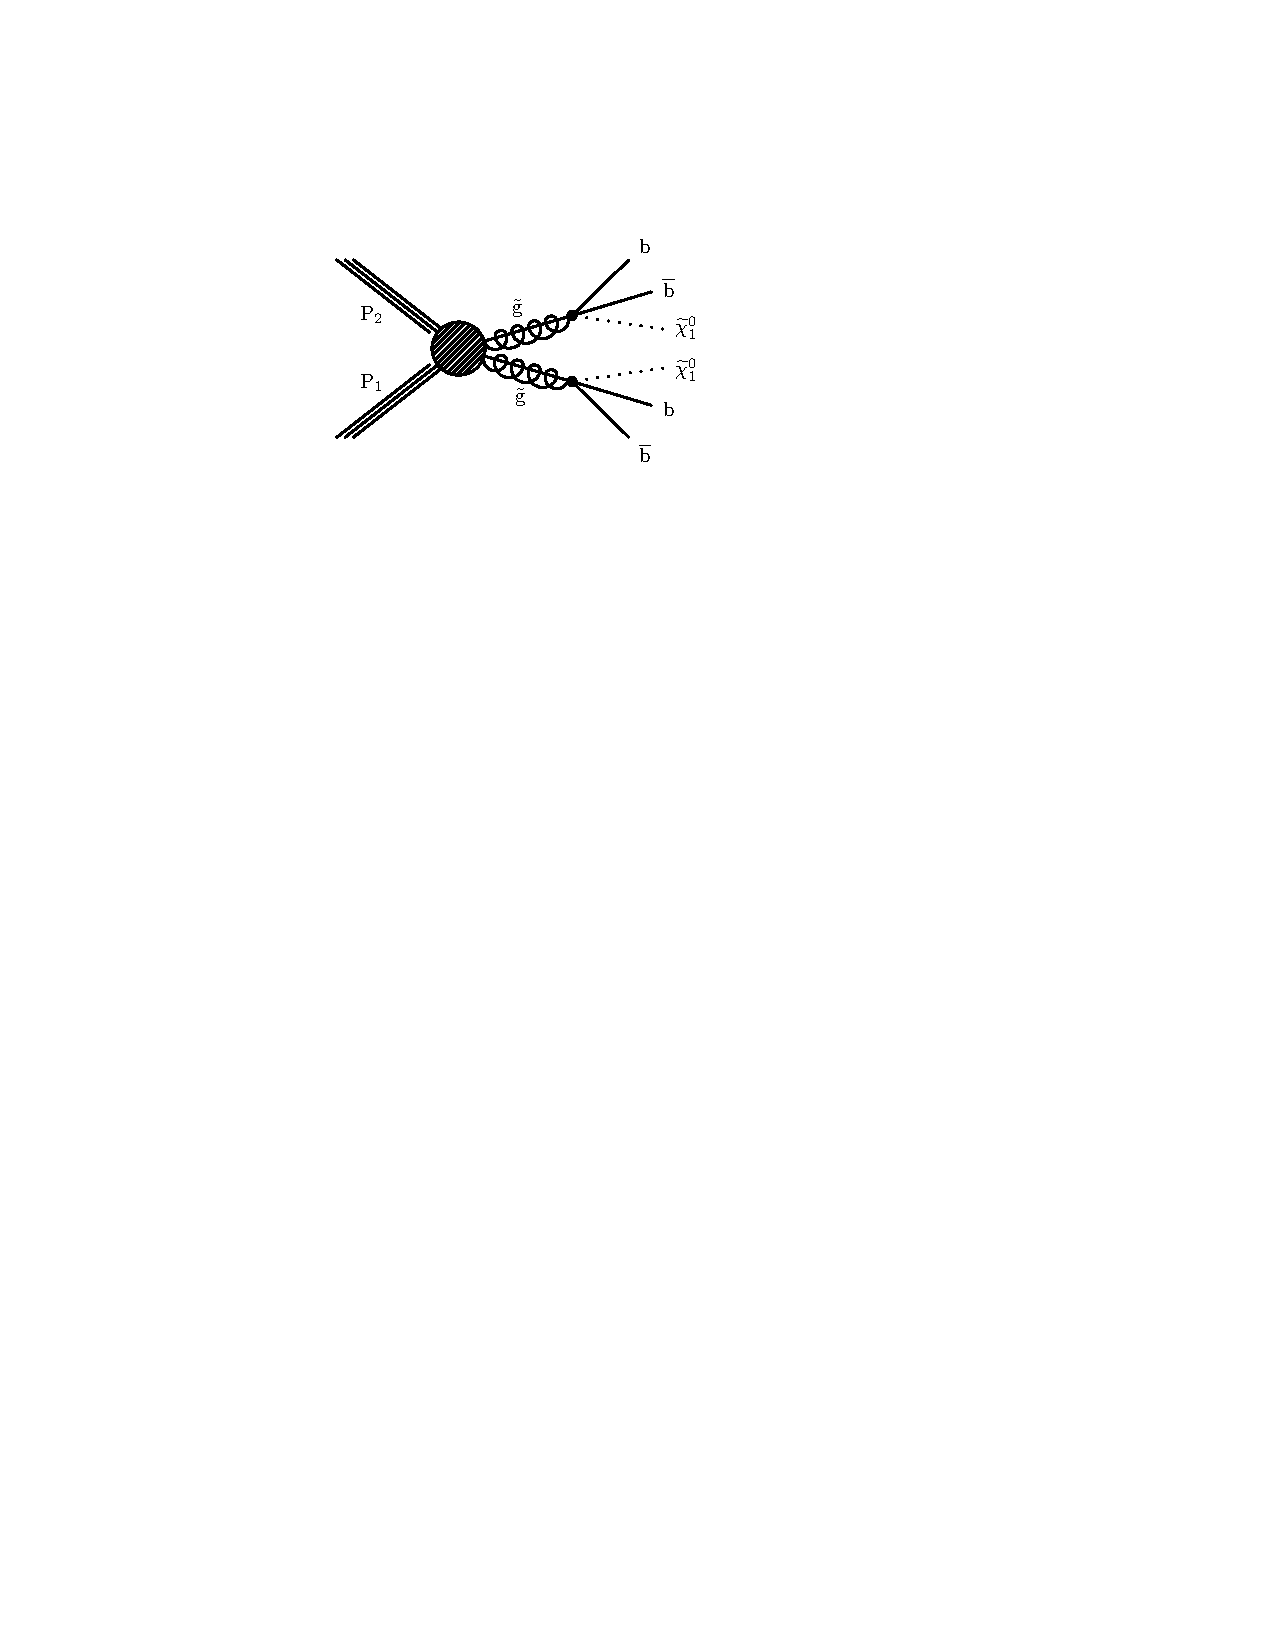
\includegraphics[width=0.30\textwidth]{results/figs/T1bbbb}
	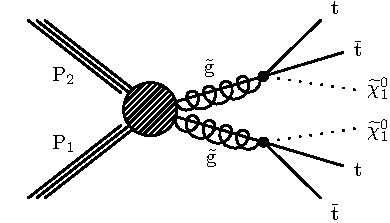
\includegraphics[width=0.30\textwidth]{results/figs/T1tttt}
	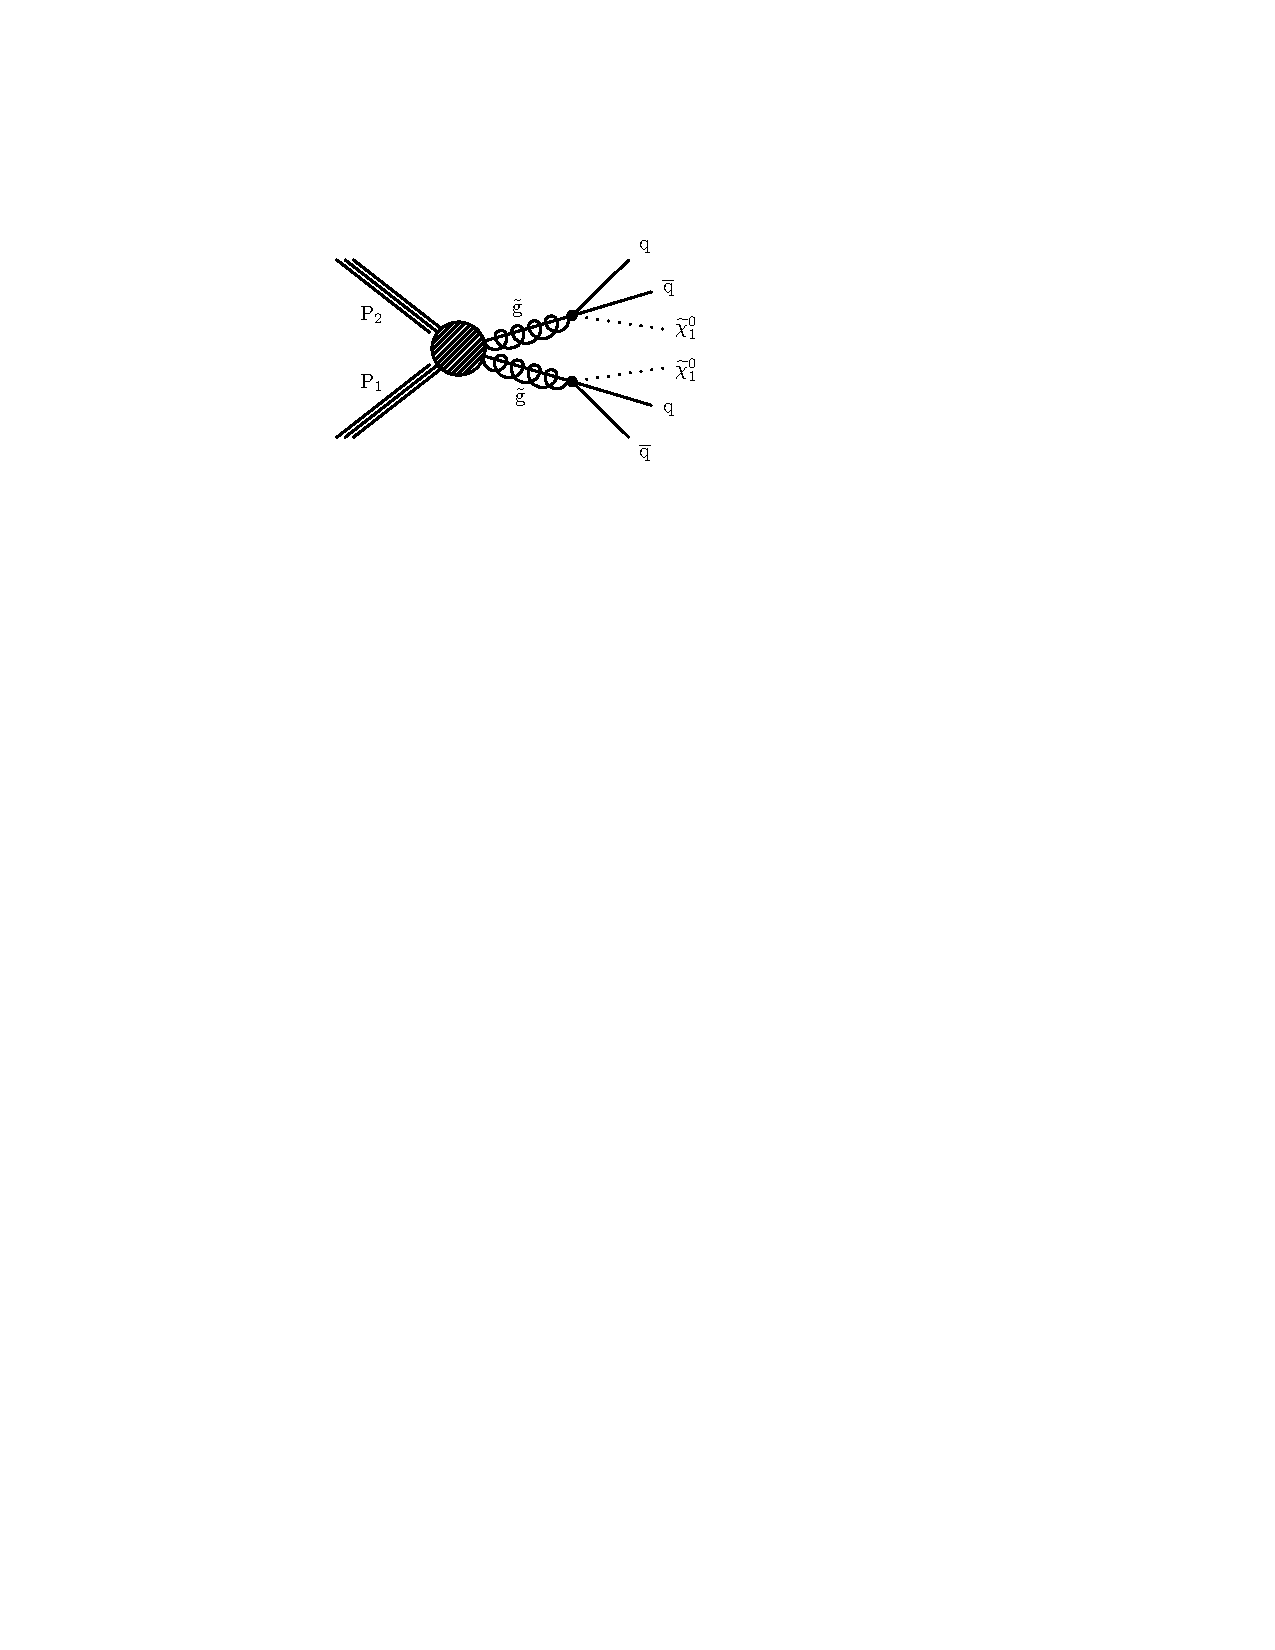
\includegraphics[width=0.30\textwidth]{results/figs/T1qqqq}
	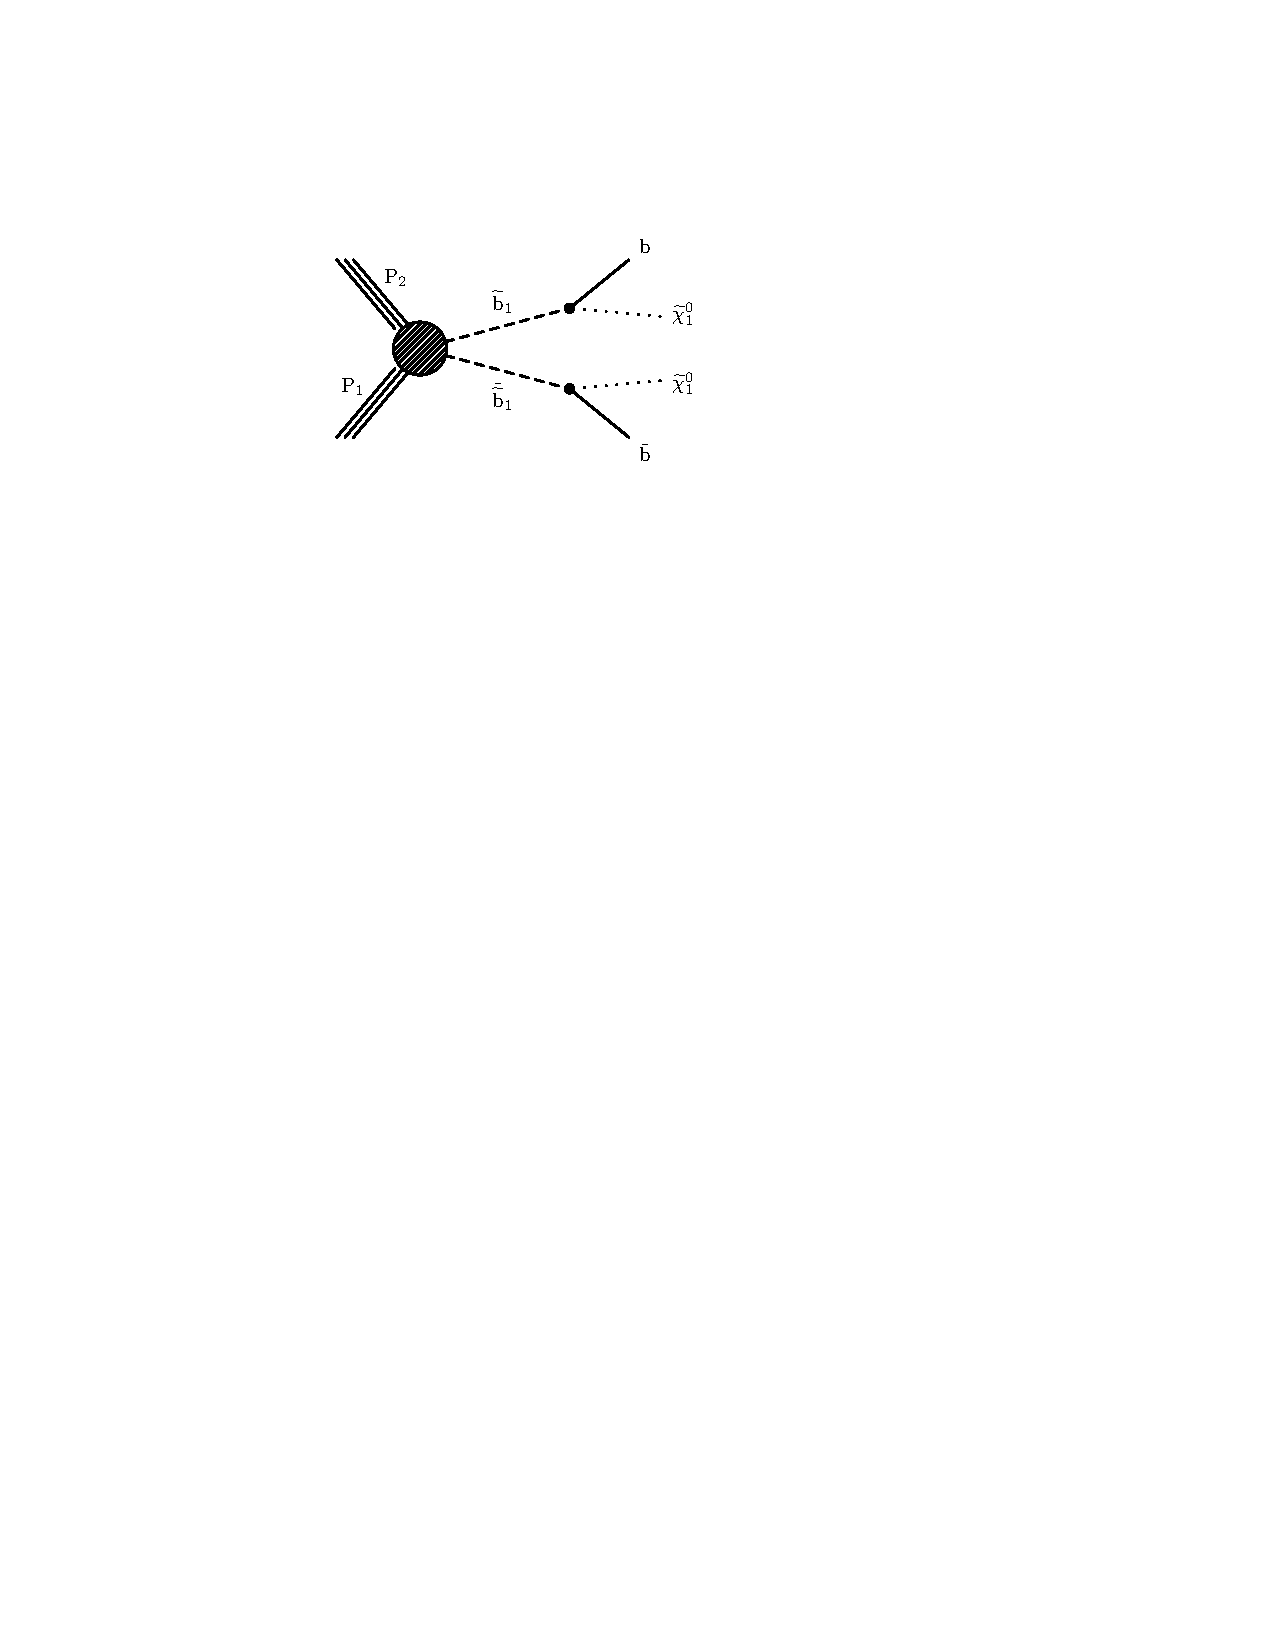
\includegraphics[width=0.30\textwidth]{results/figs/T2bb}
	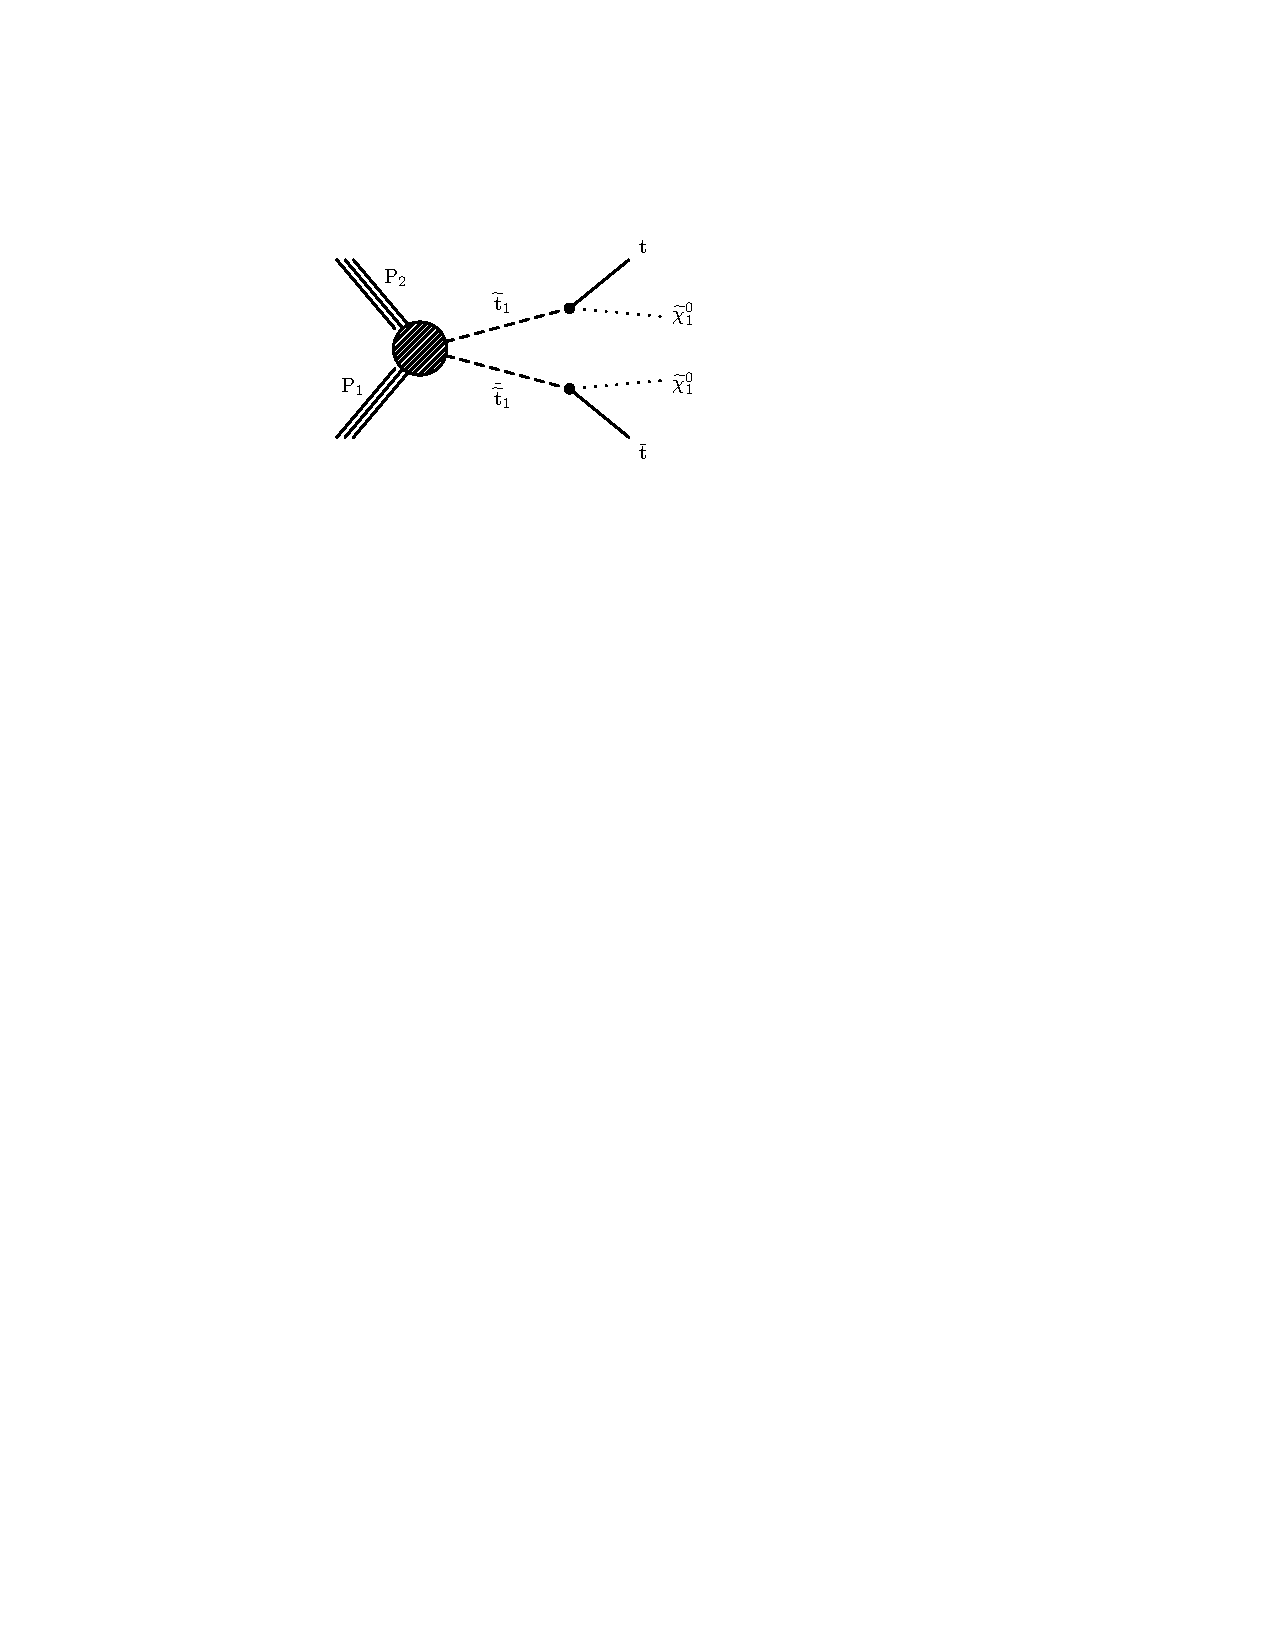
\includegraphics[width=0.30\textwidth]{results/figs/T2tt}
	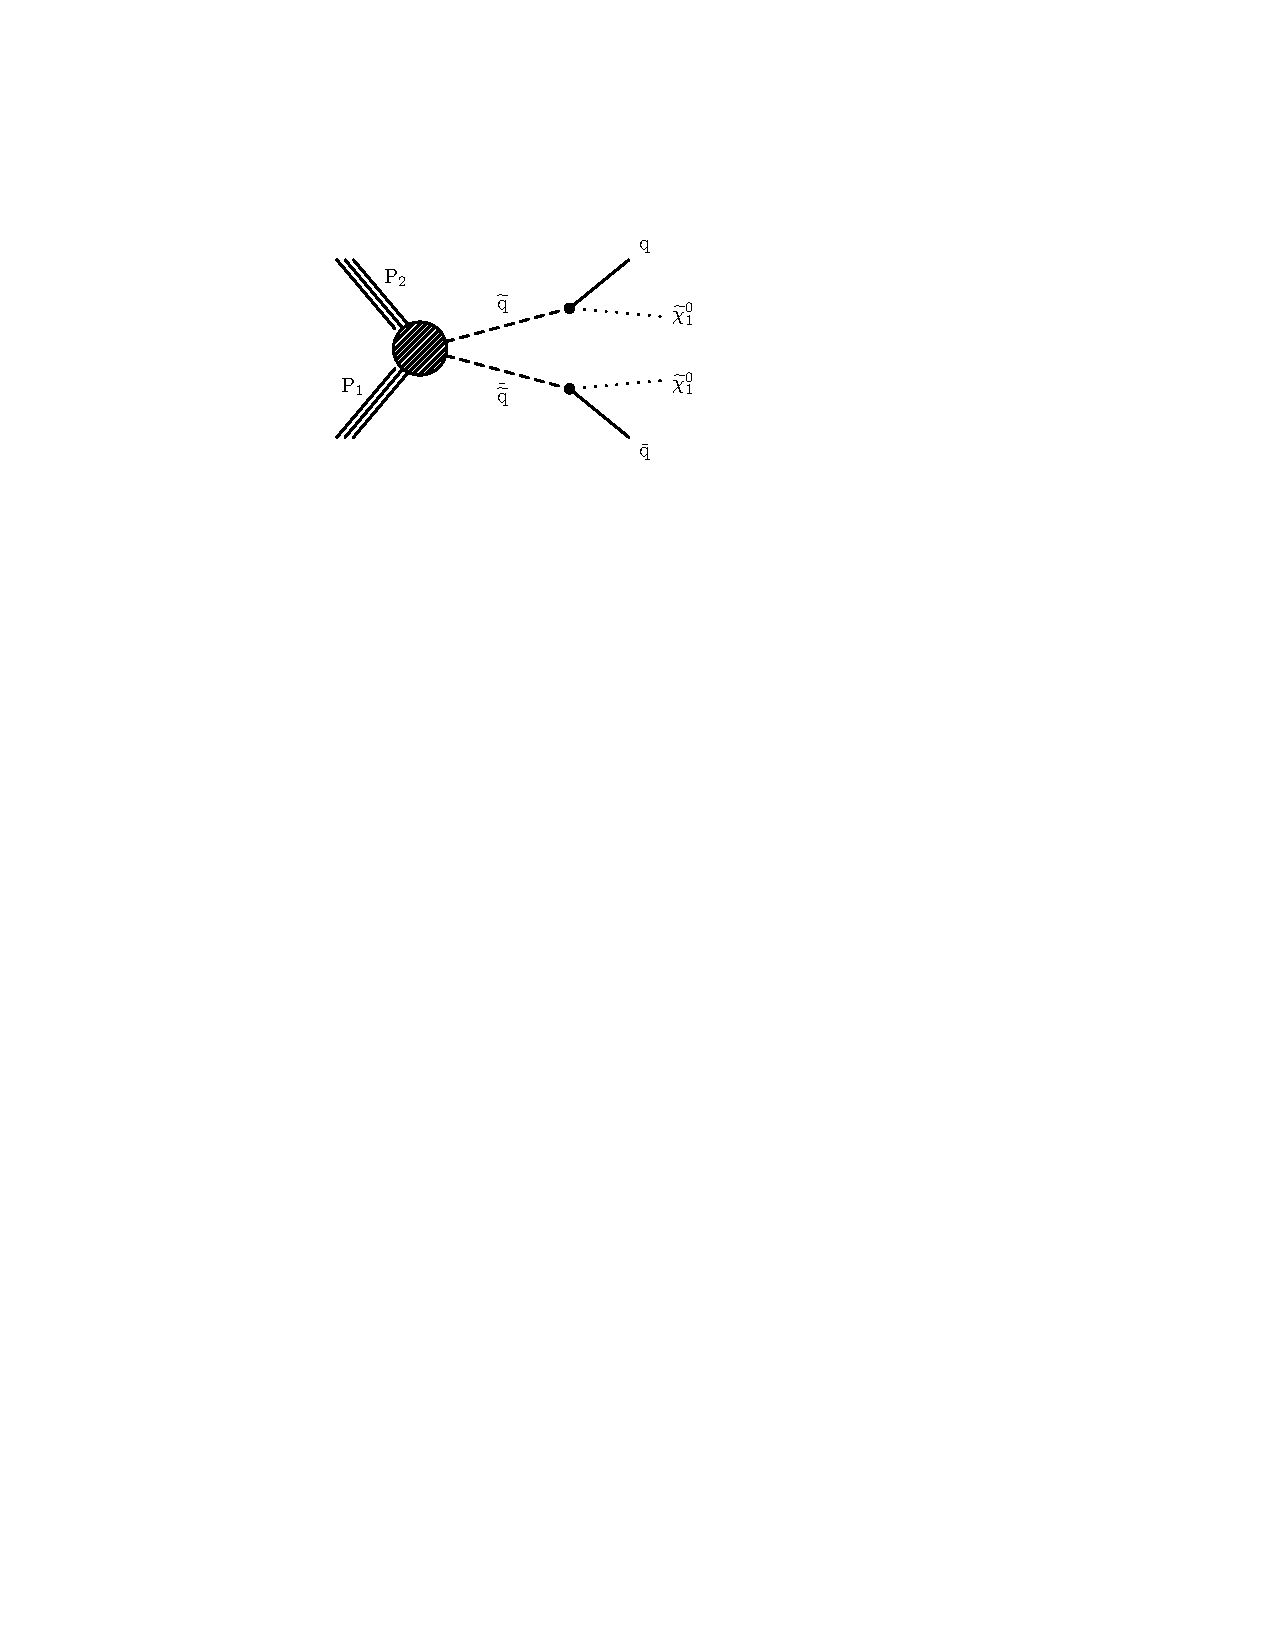
\includegraphics[width=0.30\textwidth]{results/figs/T2qq}
	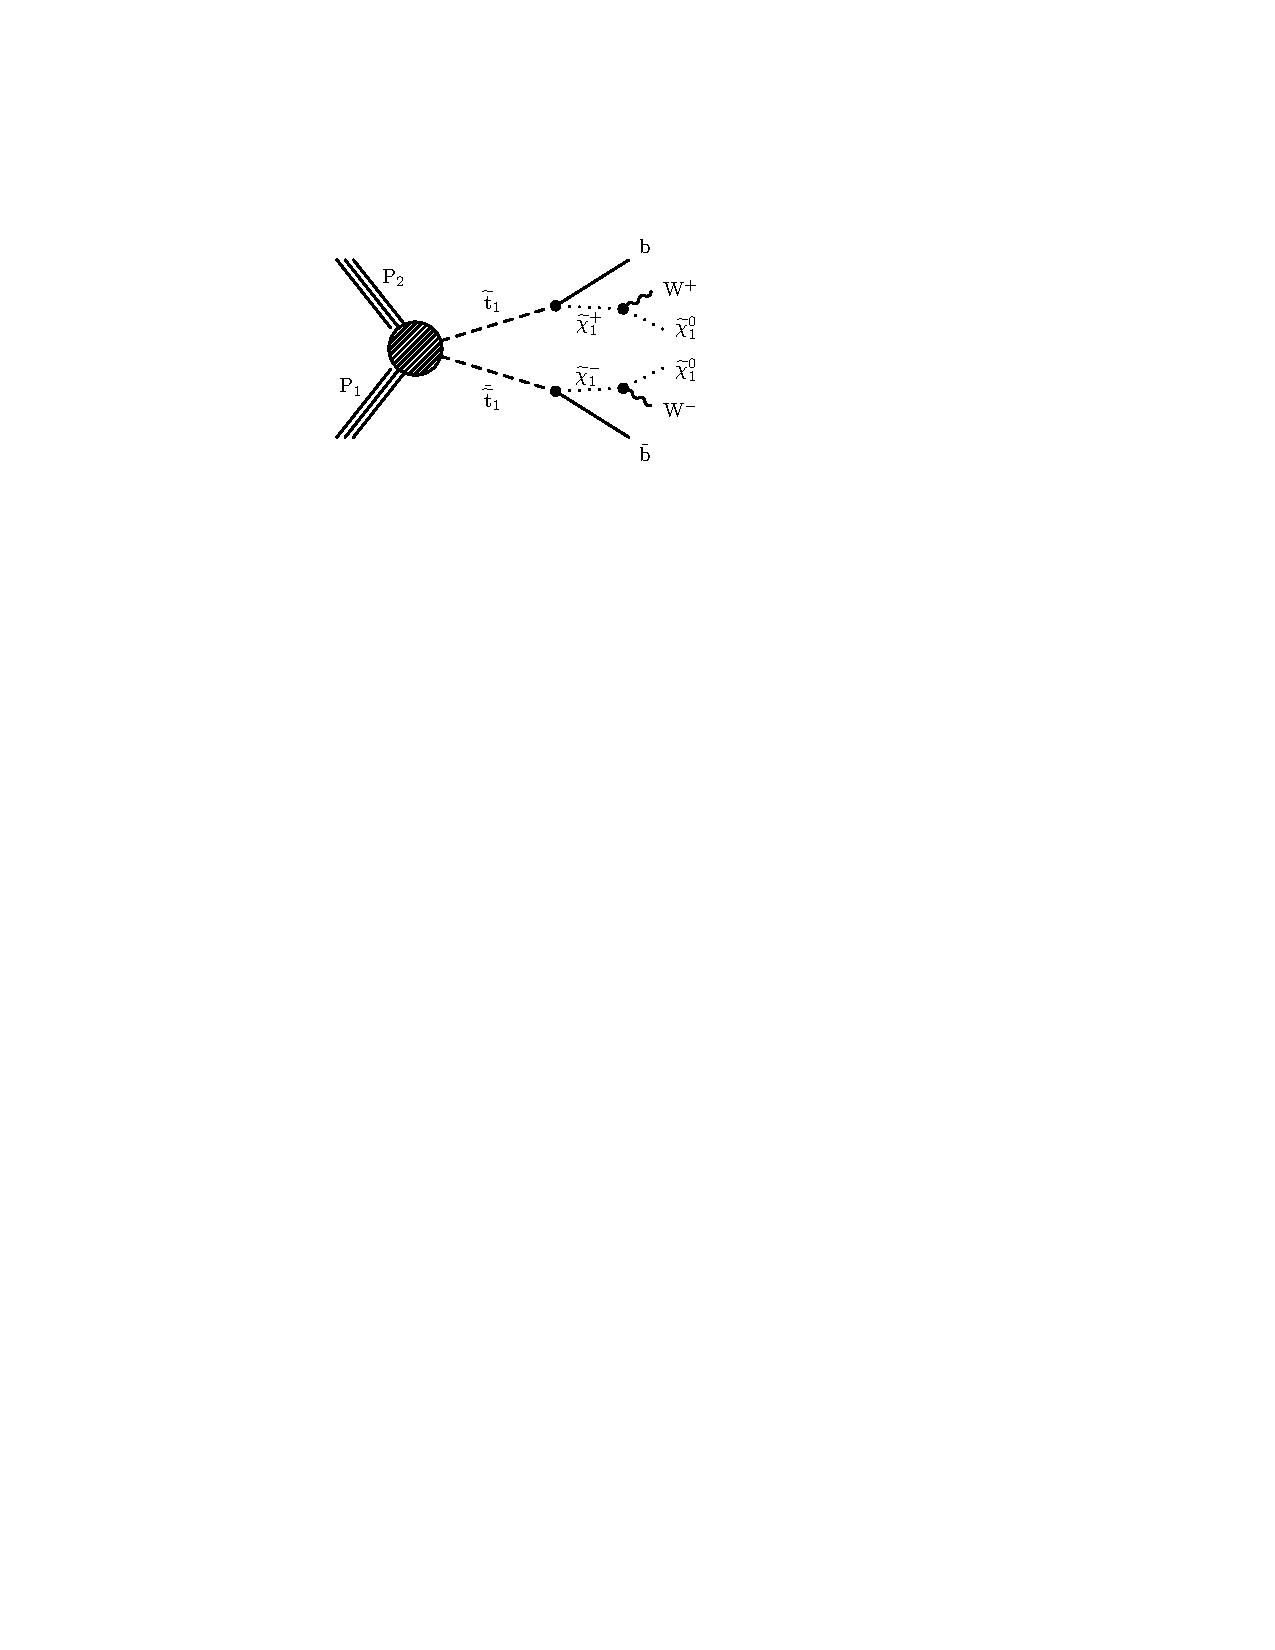
\includegraphics[width=0.30\textwidth]{results/figs/T2bw}
	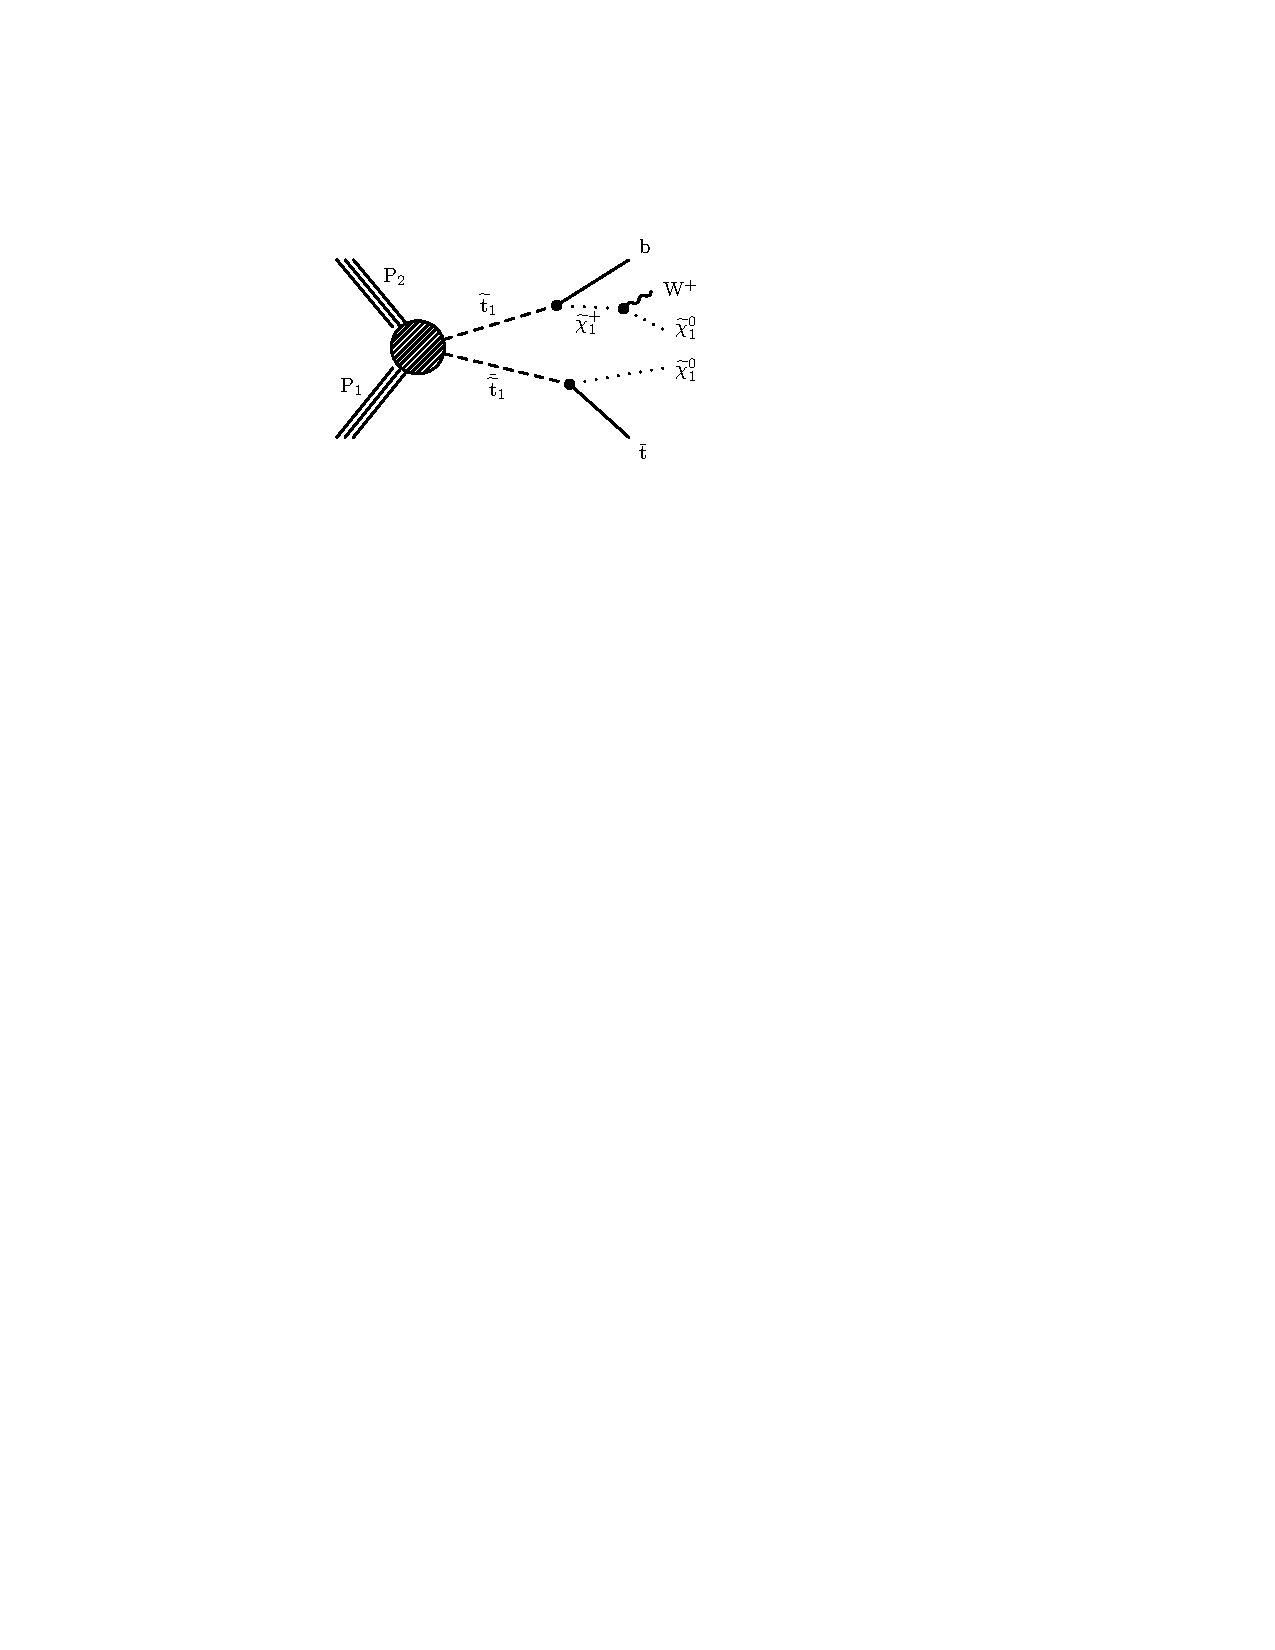
\includegraphics[width=0.30\textwidth]{results/figs/T2tb}
	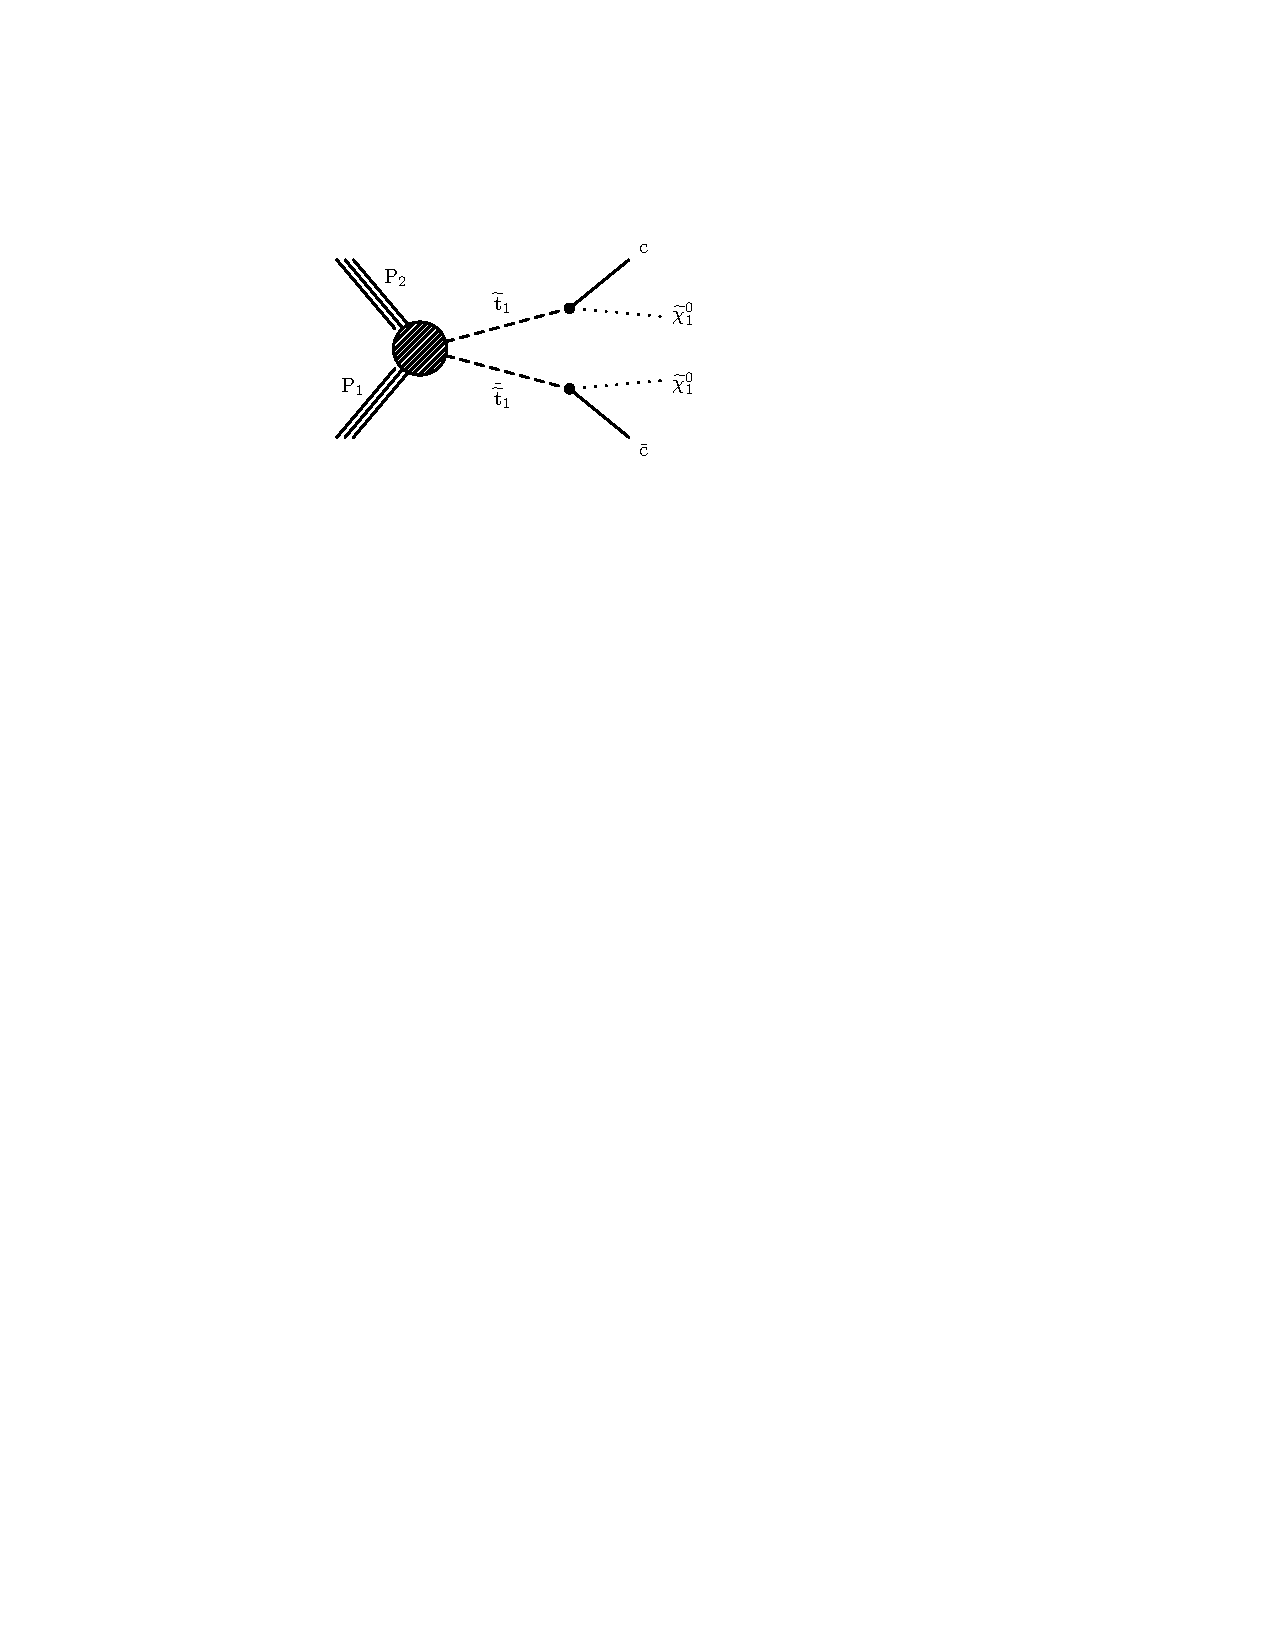
\includegraphics[width=0.30\textwidth]{results/figs/T2cc}
	\caption{Feynman diagams depicting the different simplified SUSY models considered in this analysis. Results are interpreted in the context of gluino-mediated bottom, top, and light-flavor squark production (top), direct production of bottom, top, and light-flavor squarks (middle), and alternate decay modes of direct top squark production (bottom).}
	\label{fig:signalFeynman}
\end{figure}

The cross-section exclusion limits are calculated at 95\% confidence level (CL) for each simplified model. The limits are obtained using the background-fitting procedure described in section \ref{sec:yields} obtained with the higgsCombine tool. The 95\% CL exclusion limits for gluino-mediated models is shown in figure \ref{fig:limitsGluino}, for direct squark production in figure \ref{fig:limitsSquark}, and for alternate top squark decay modes in figure \ref{fig:limitsStop}. The constraints on the masses of SUSY particles excluded by this search is summarized in table \ref{tbl:limits}.
\begin{figure}
	\centering
	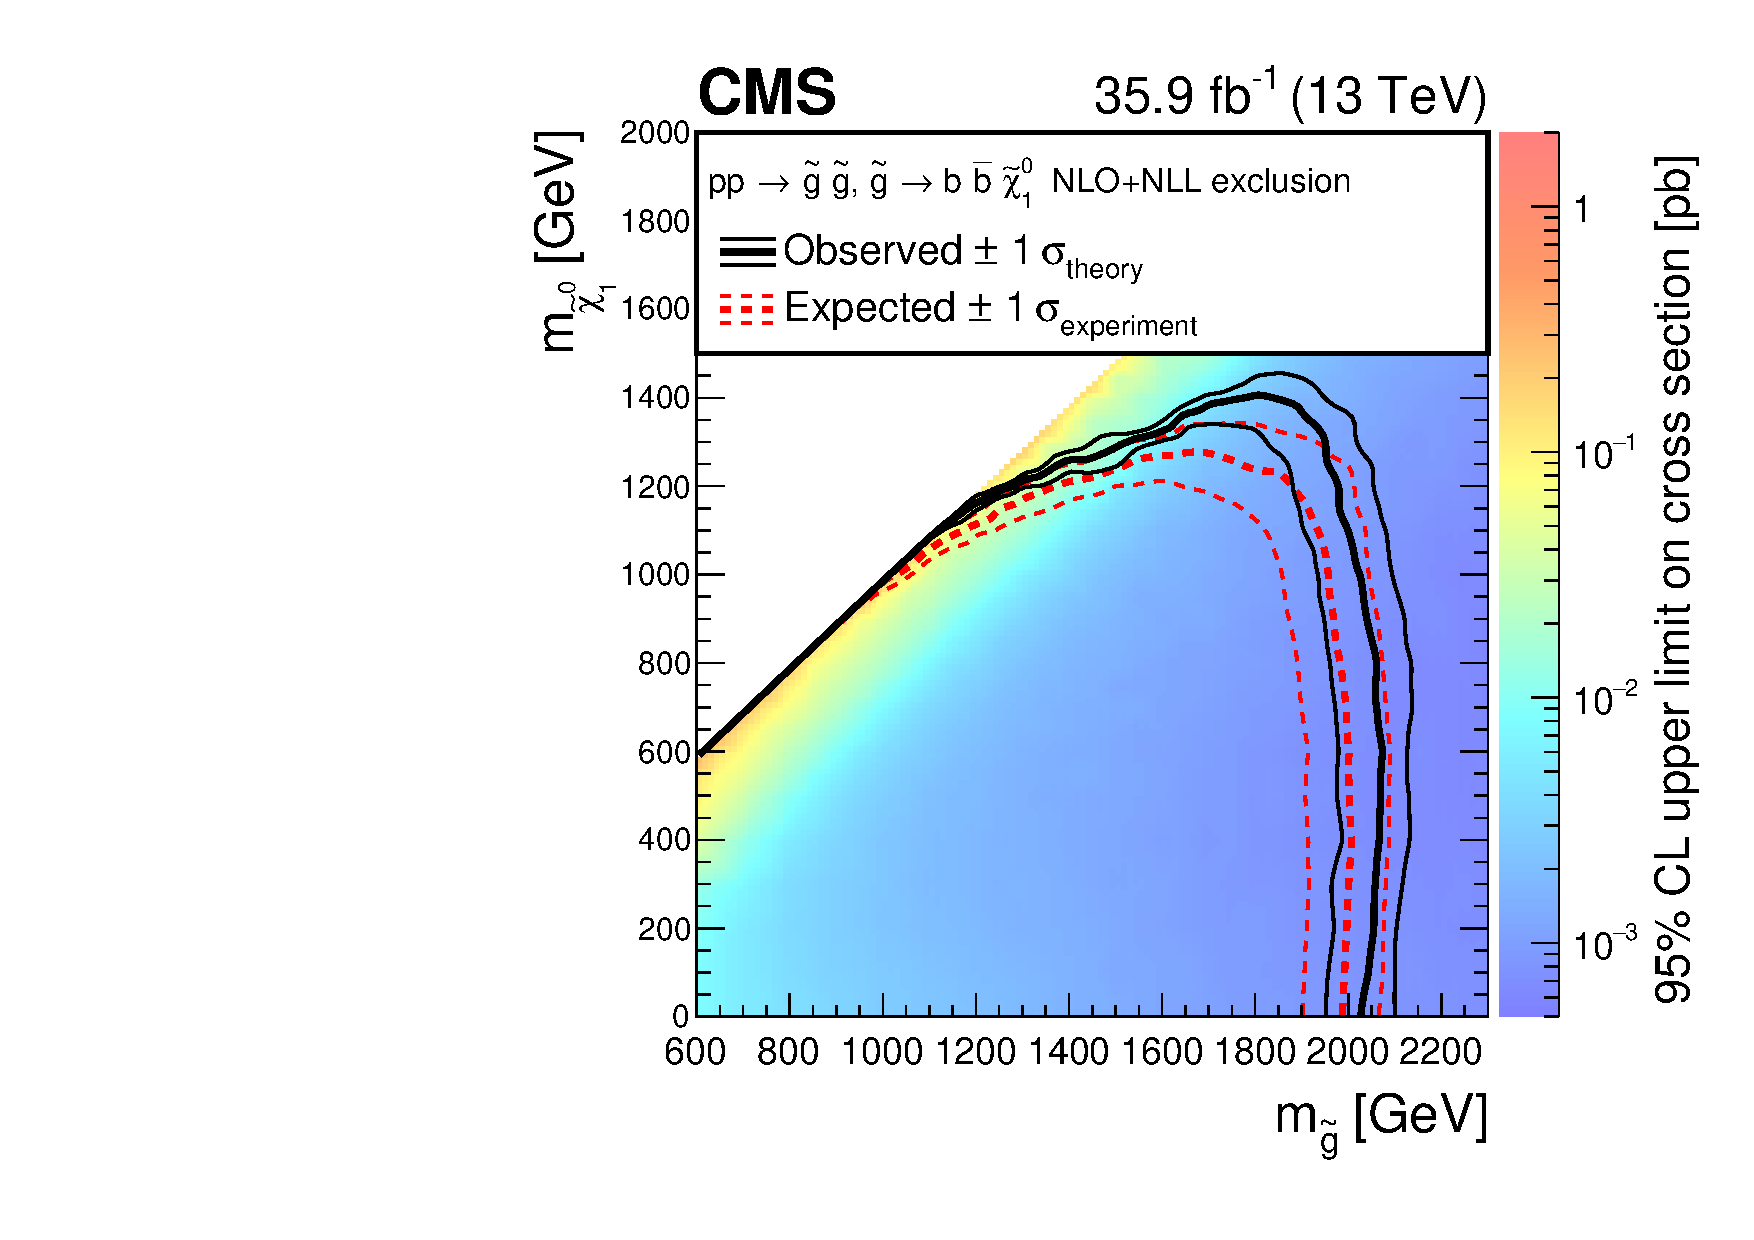
\includegraphics[width=0.45\textwidth]{results/figs/interpretations/T1bbbb_35p9ifb_Moriond2017_Mar07_XSEC}
	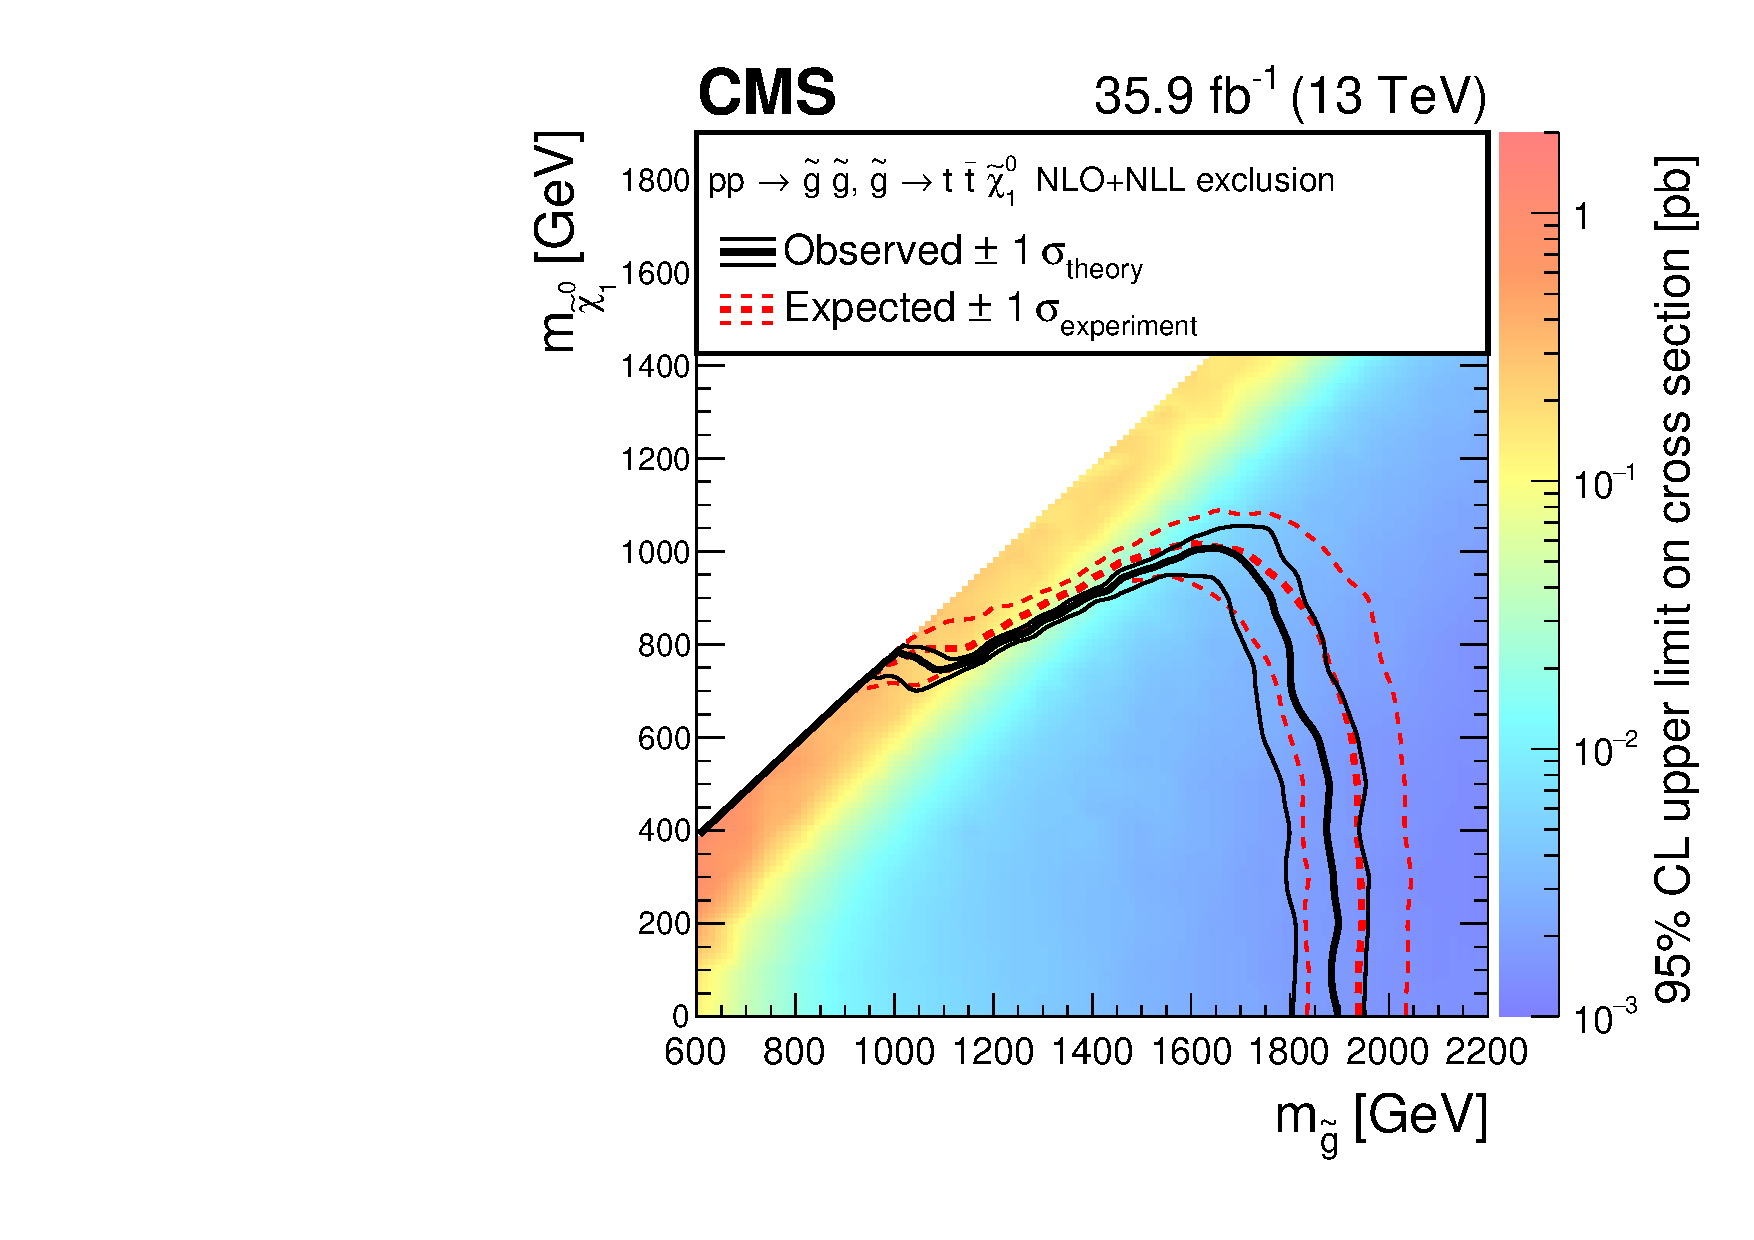
\includegraphics[width=0.45\textwidth]{results/figs/interpretations/T1tttt_35p9ifb_Moriond2017_Mar07_XSEC}
	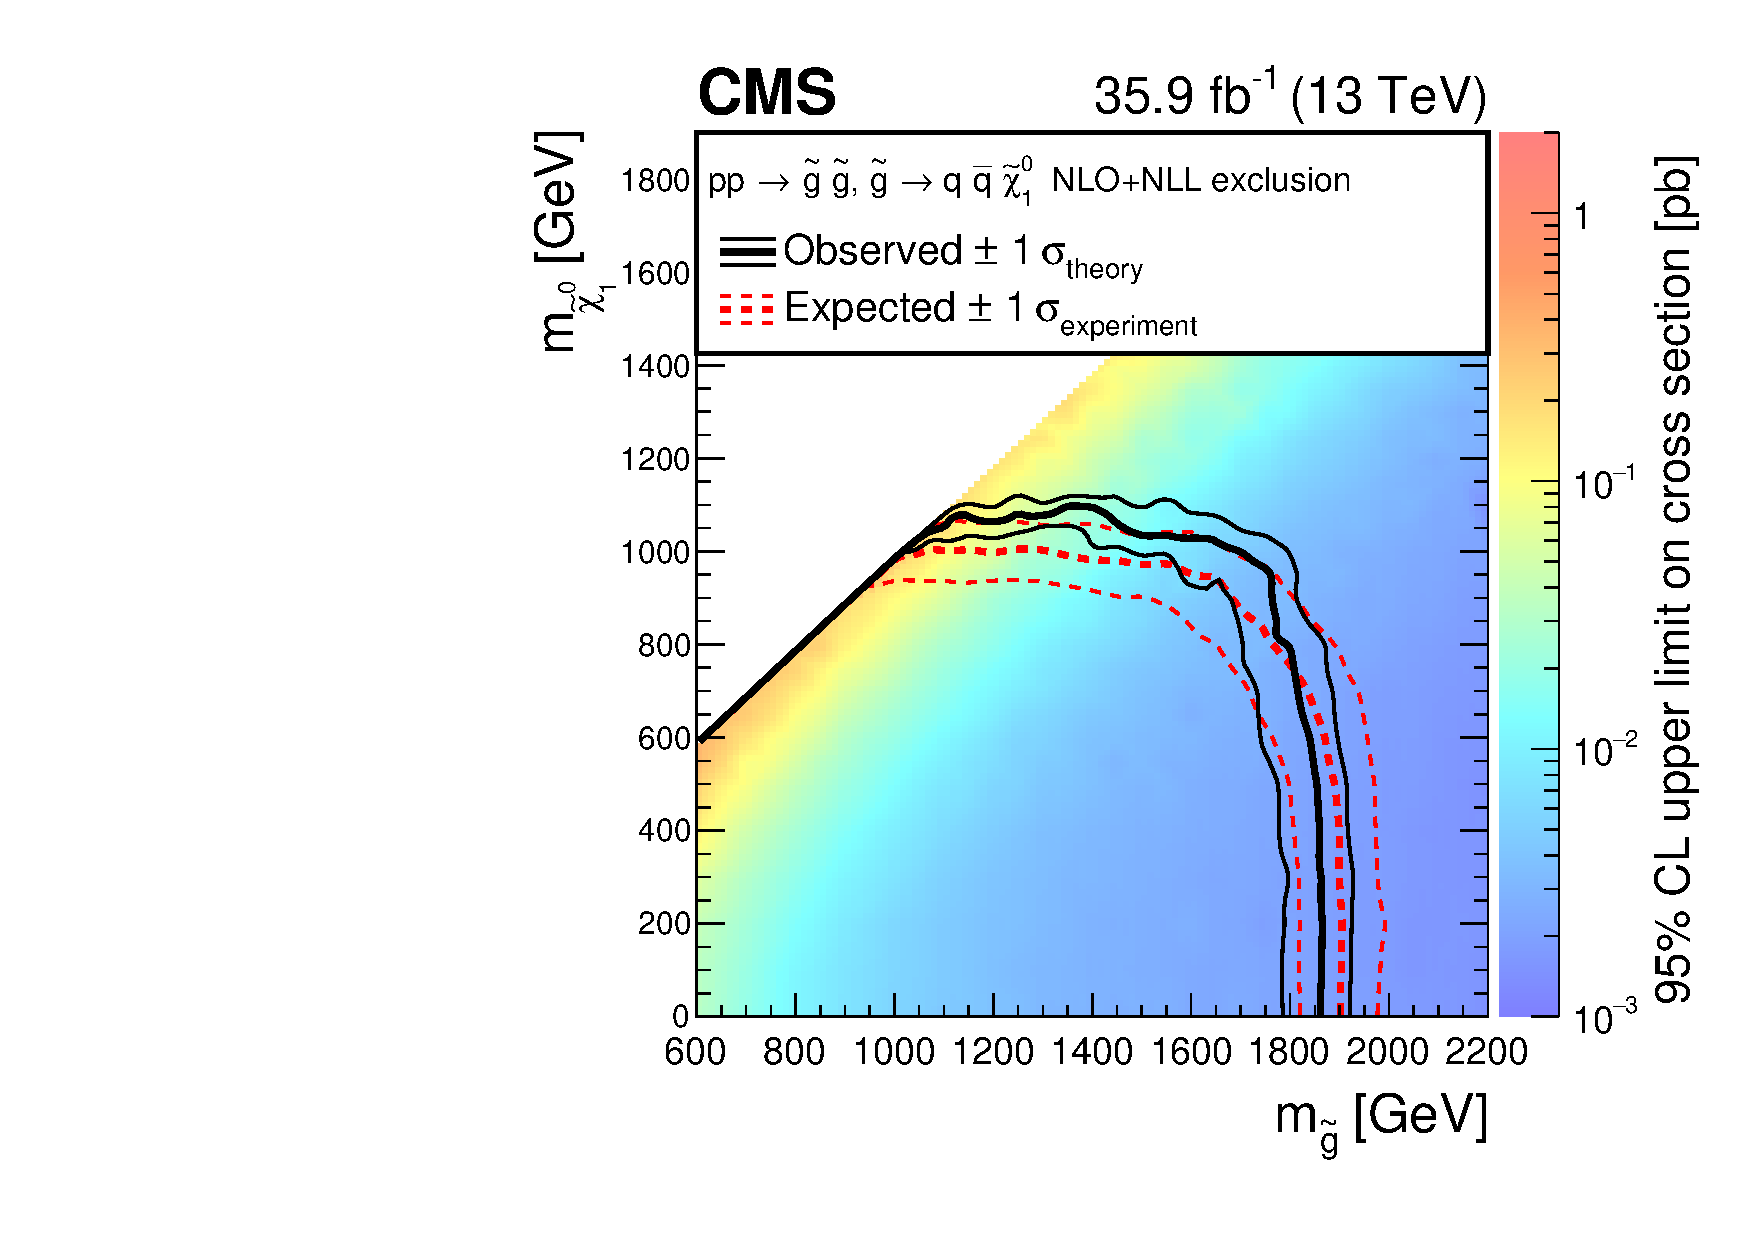
\includegraphics[width=0.45\textwidth]{results/figs/interpretations/T1qqqq_35p9ifb_Moriond2017_Mar07_XSEC}
	\caption{Exclusion limits at 95\% confidence level for gluino-mediated squark production of bottom (top left), top (top right), and light-flavor (bottom) squarks. The dashed red lines indicate the expected sensitivity and associated uncertainty, while the black lines indicate the observed exclusion limit and its associated theoretical uncertainty based on the signal cross-section.}
	\label{fig:limitsGluino}
\end{figure}
\begin{figure}
	\centering
	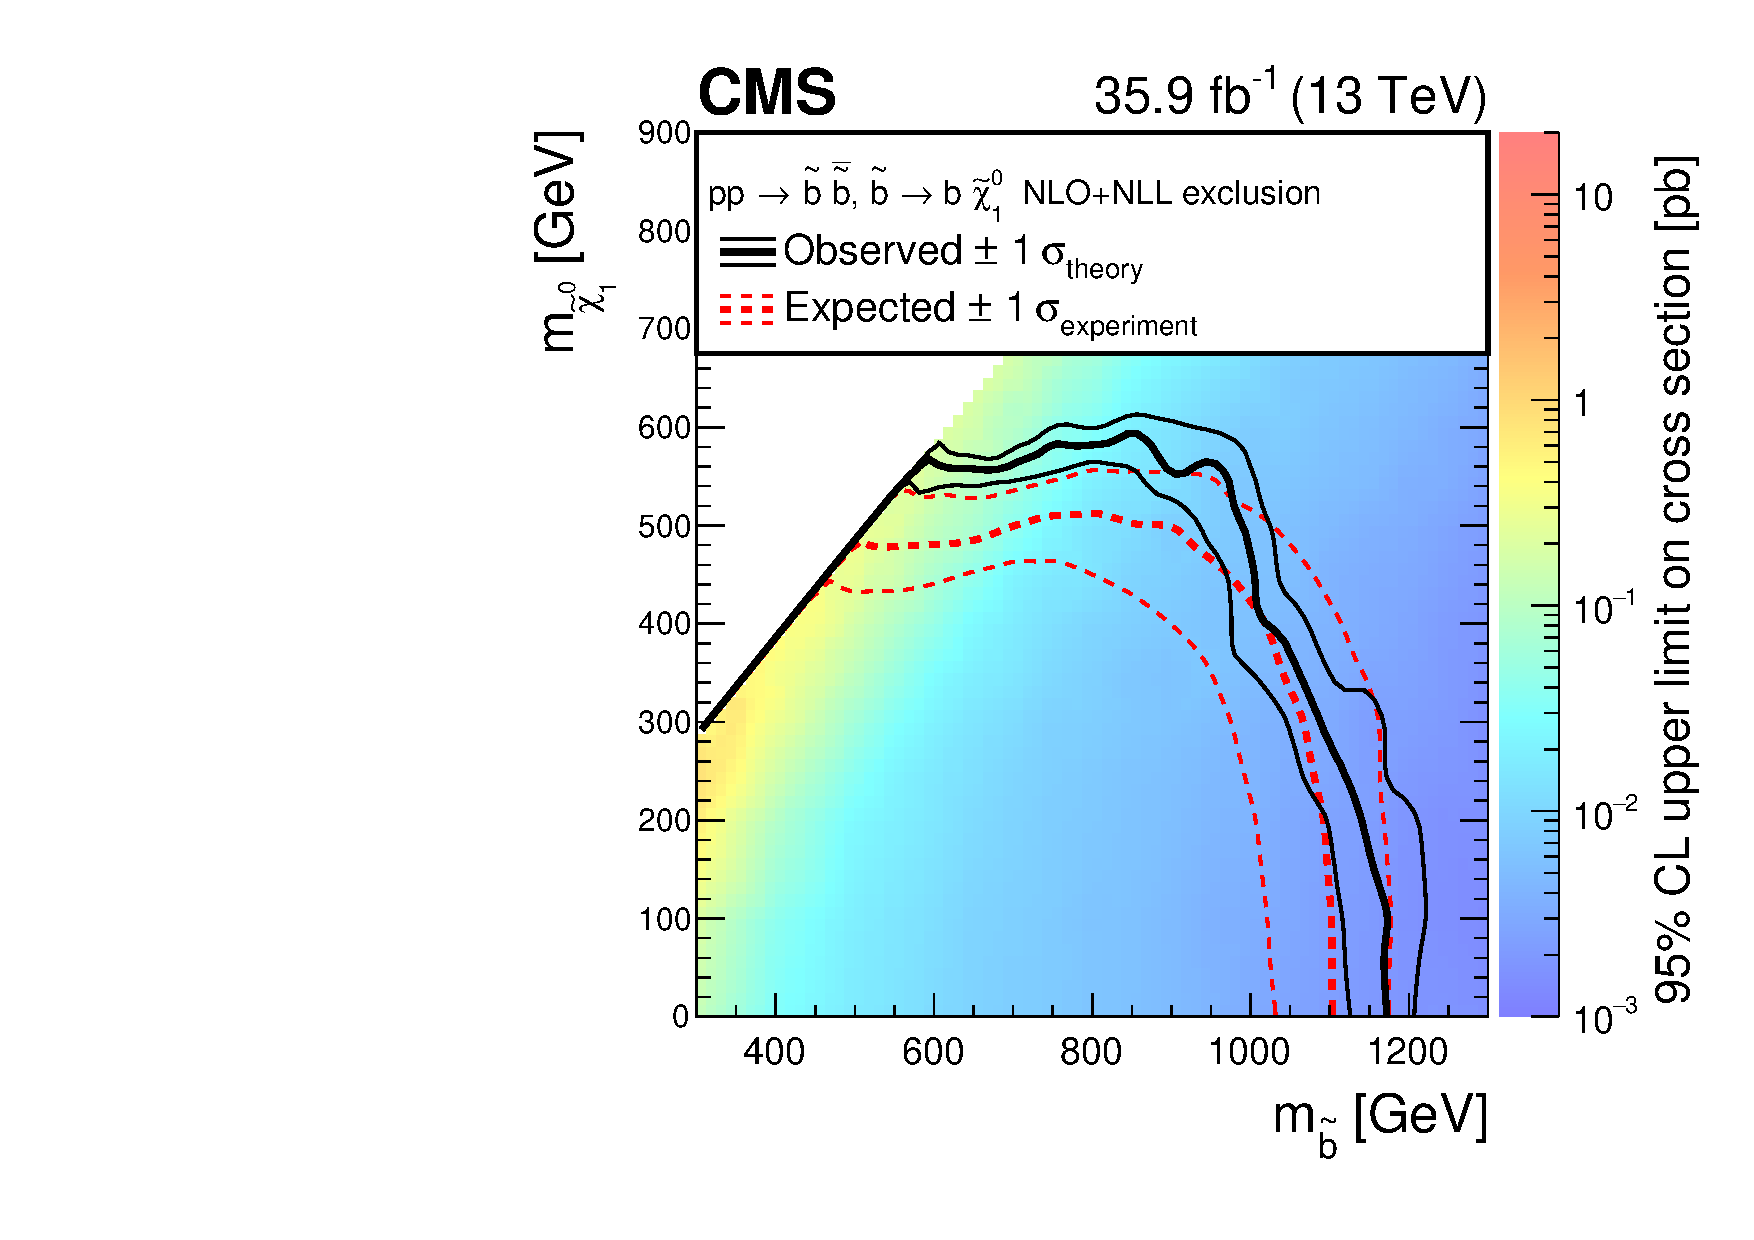
\includegraphics[width=0.45\textwidth]{results/figs/interpretations/T2bb_35p9ifb_Moriond2017_Mar07_XSEC}
	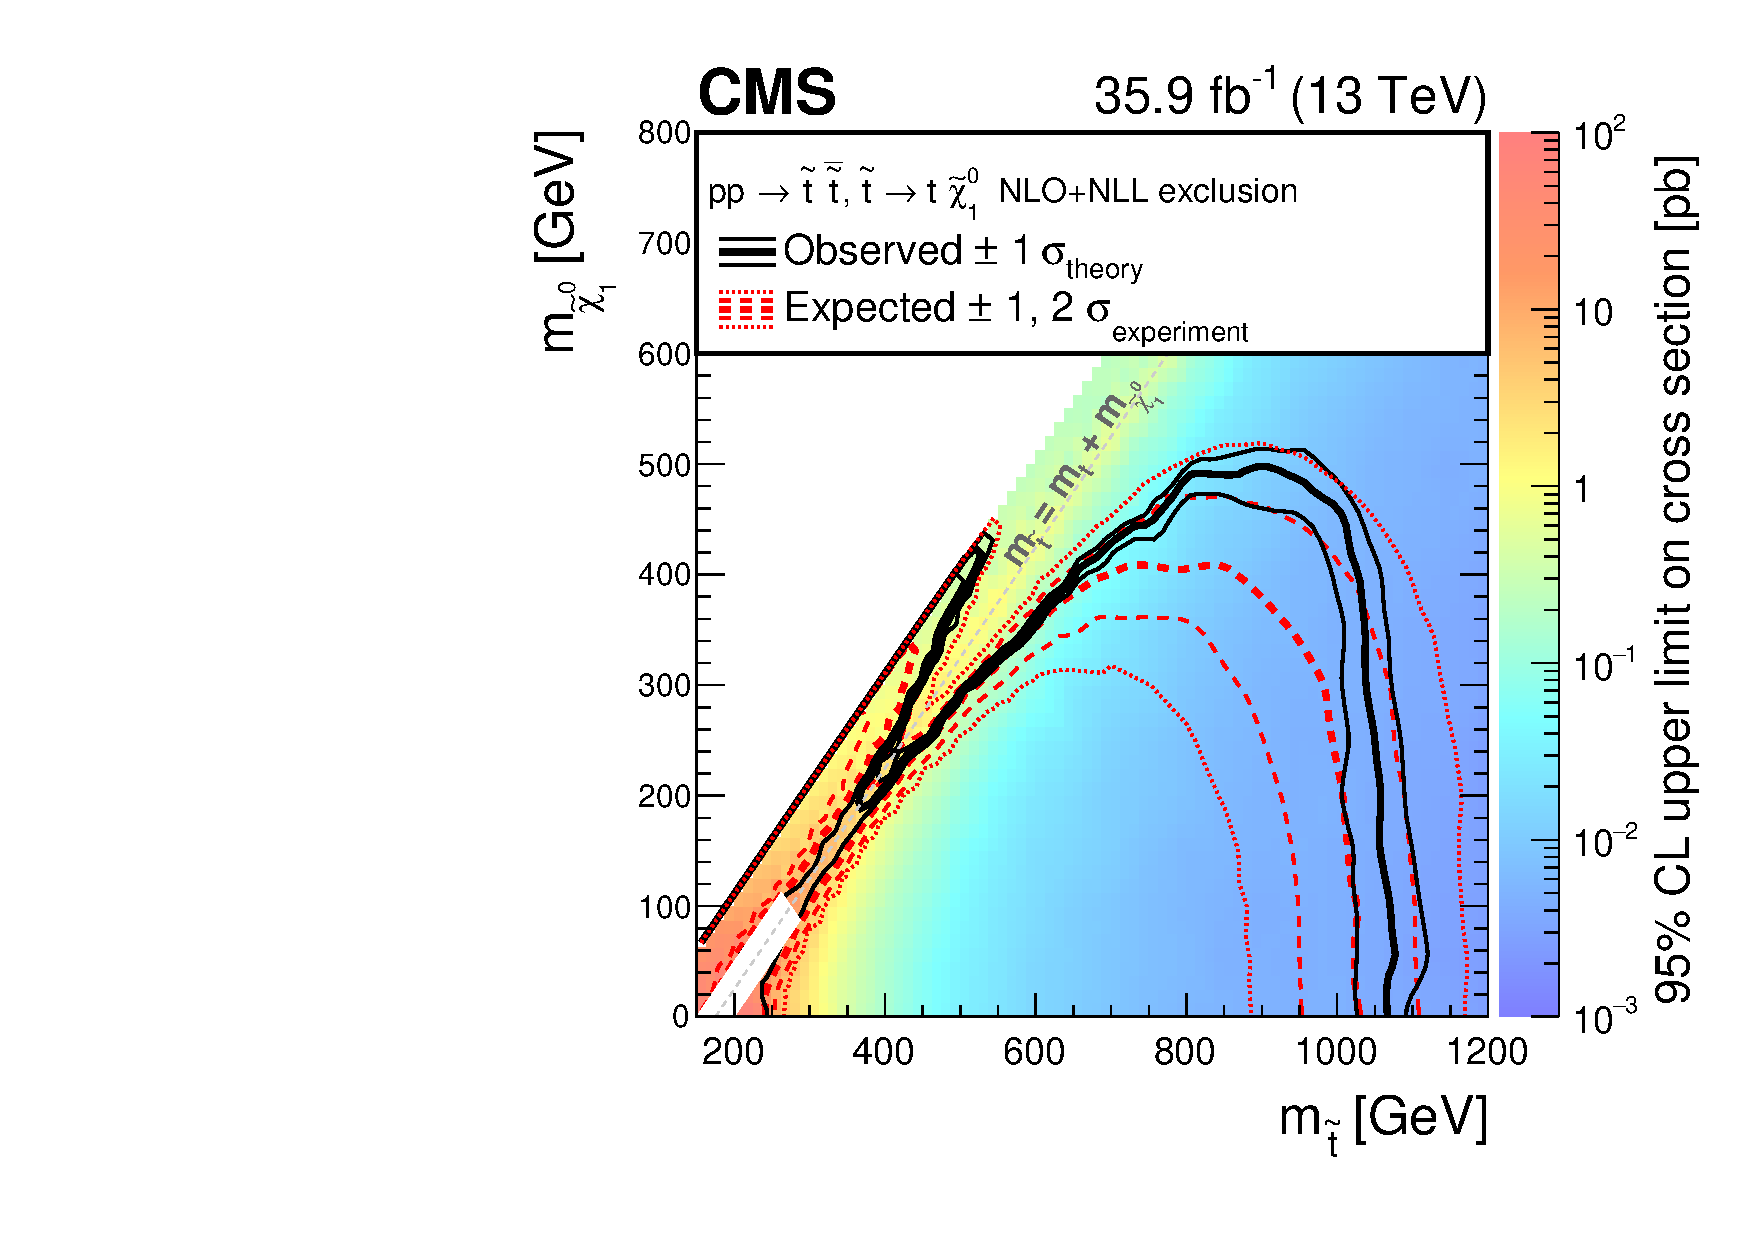
\includegraphics[width=0.45\textwidth]{results/figs/interpretations/T2tt_35p9ifb_Moriond2017_Mar07_XSEC}
	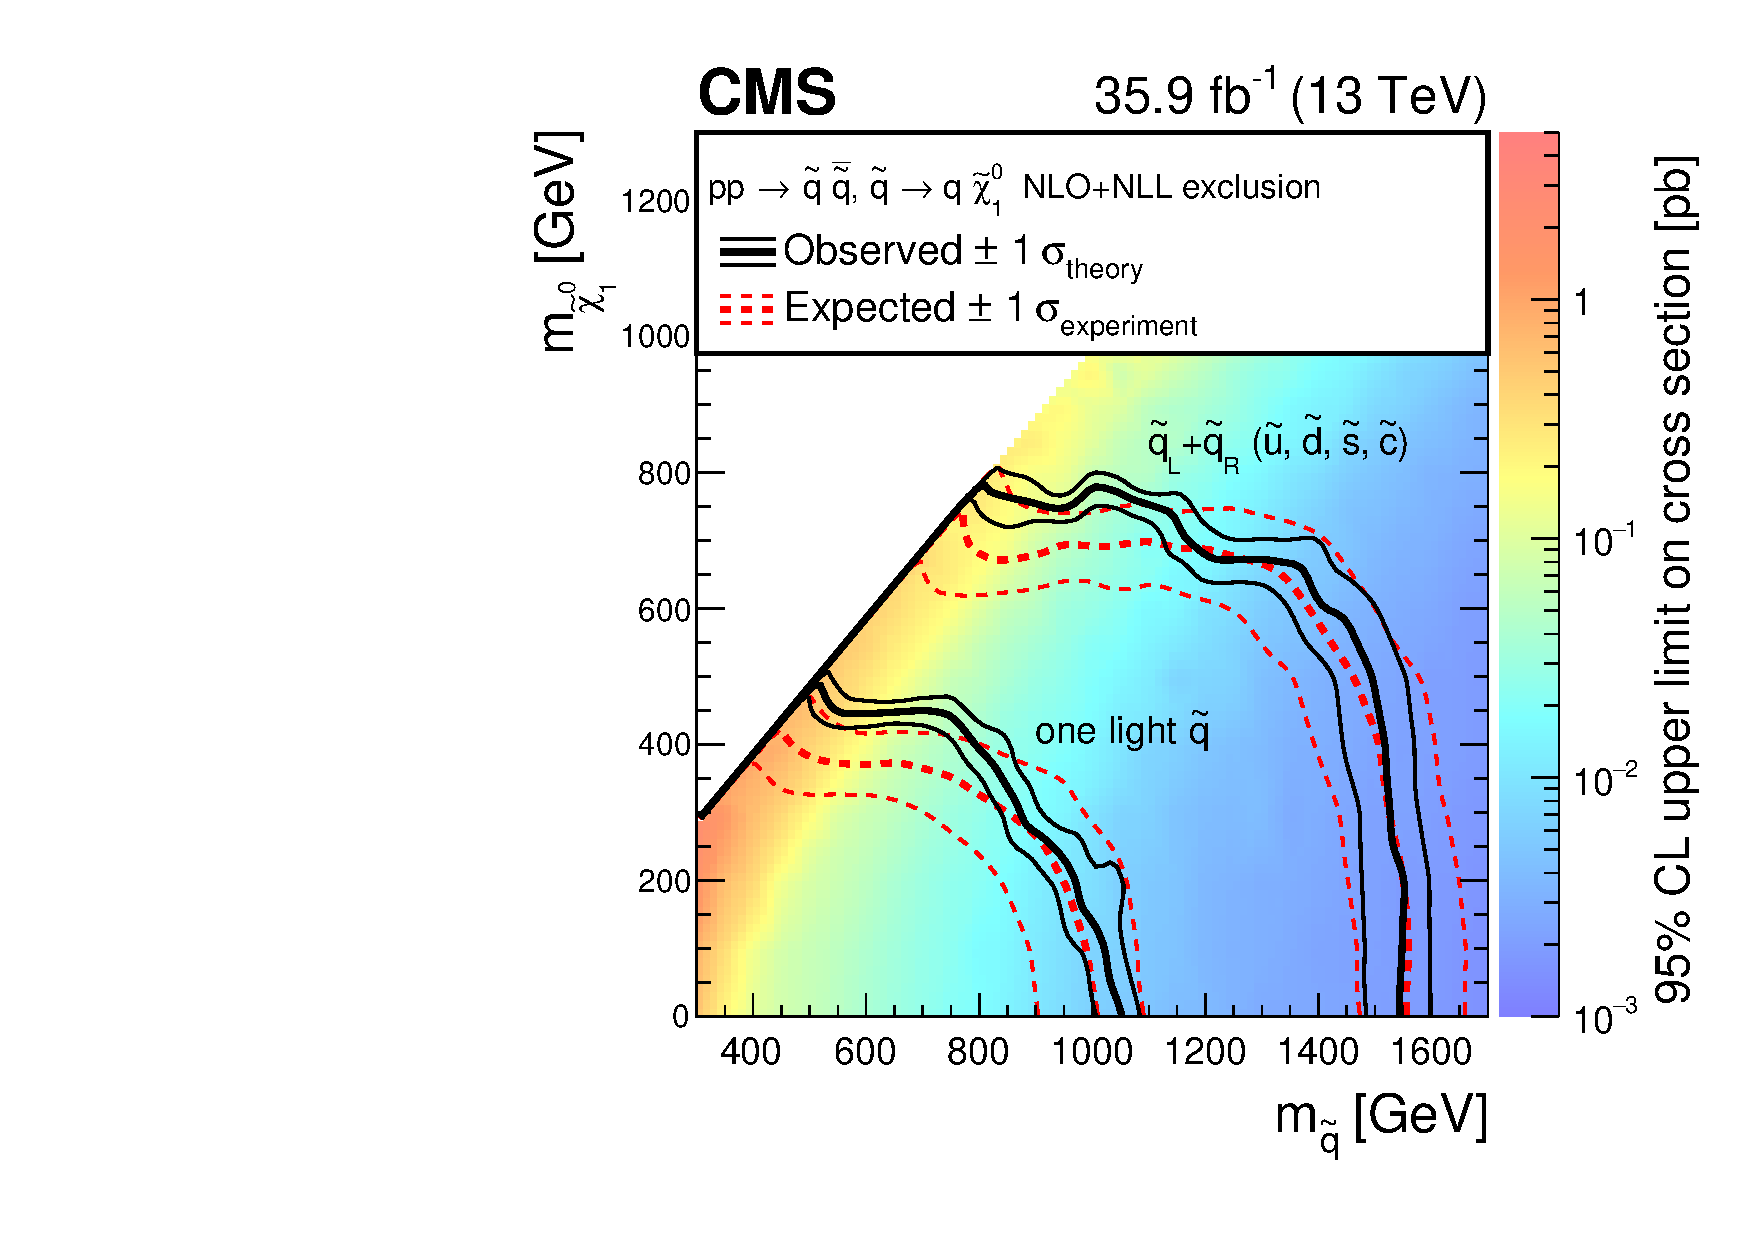
\includegraphics[width=0.45\textwidth]{results/figs/interpretations/T2qq_35p9ifb_Moriond2017_Mar07_XSEC}
	\caption{Exclusion limits at 95\% confidence level for direct squark production of bottom (top left), top (top right), and light-flavor (bottom) squarks. The dashed red lines indicate the expected sensitivity and associated uncertainty, while the black lines indicate the observed exclusion limit and its associated theoretical uncertainty based on the signal cross-section.}
	\label{fig:limitsSquark}
\end{figure}
\begin{figure}
	\centering
	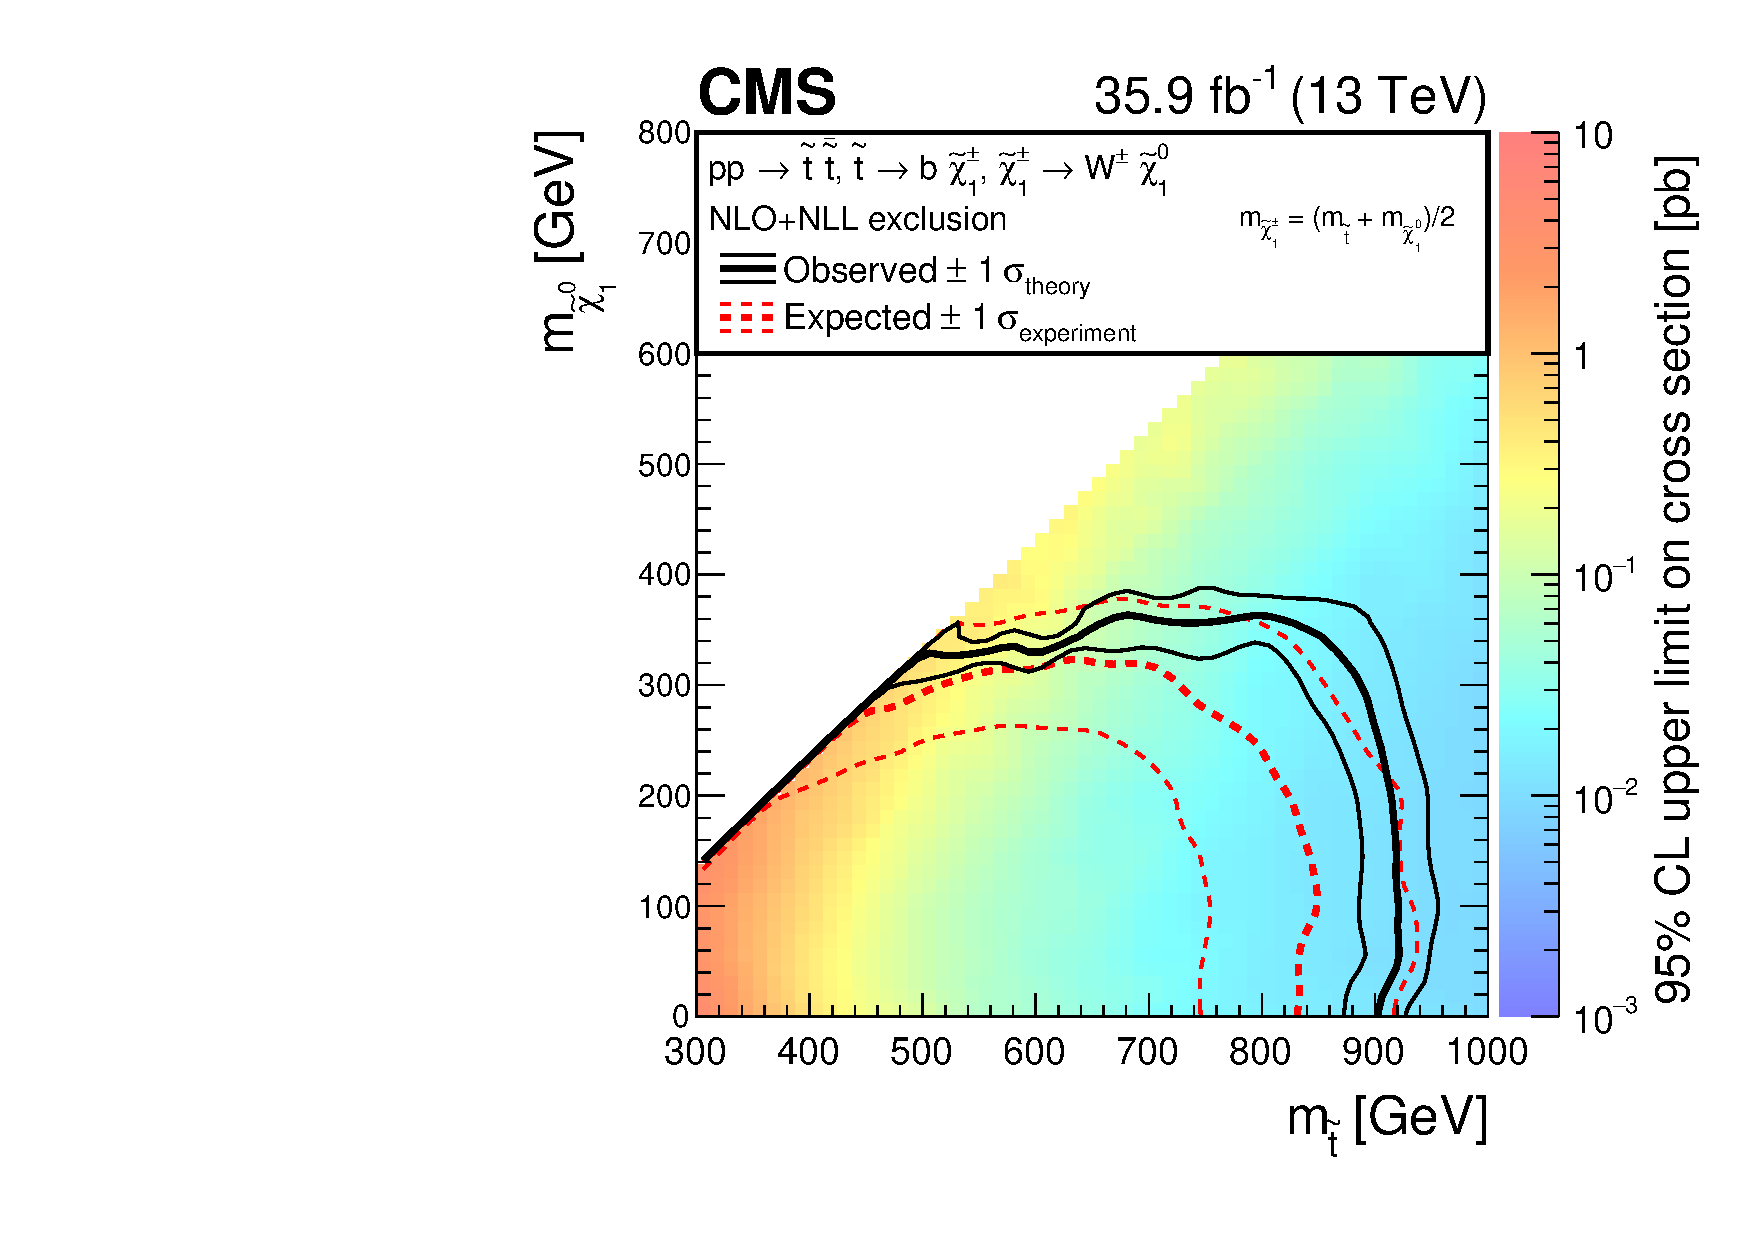
\includegraphics[width=0.45\textwidth]{results/figs/interpretations/T2bW_35p9ifb_Moriond2017_Mar07_XSEC}
	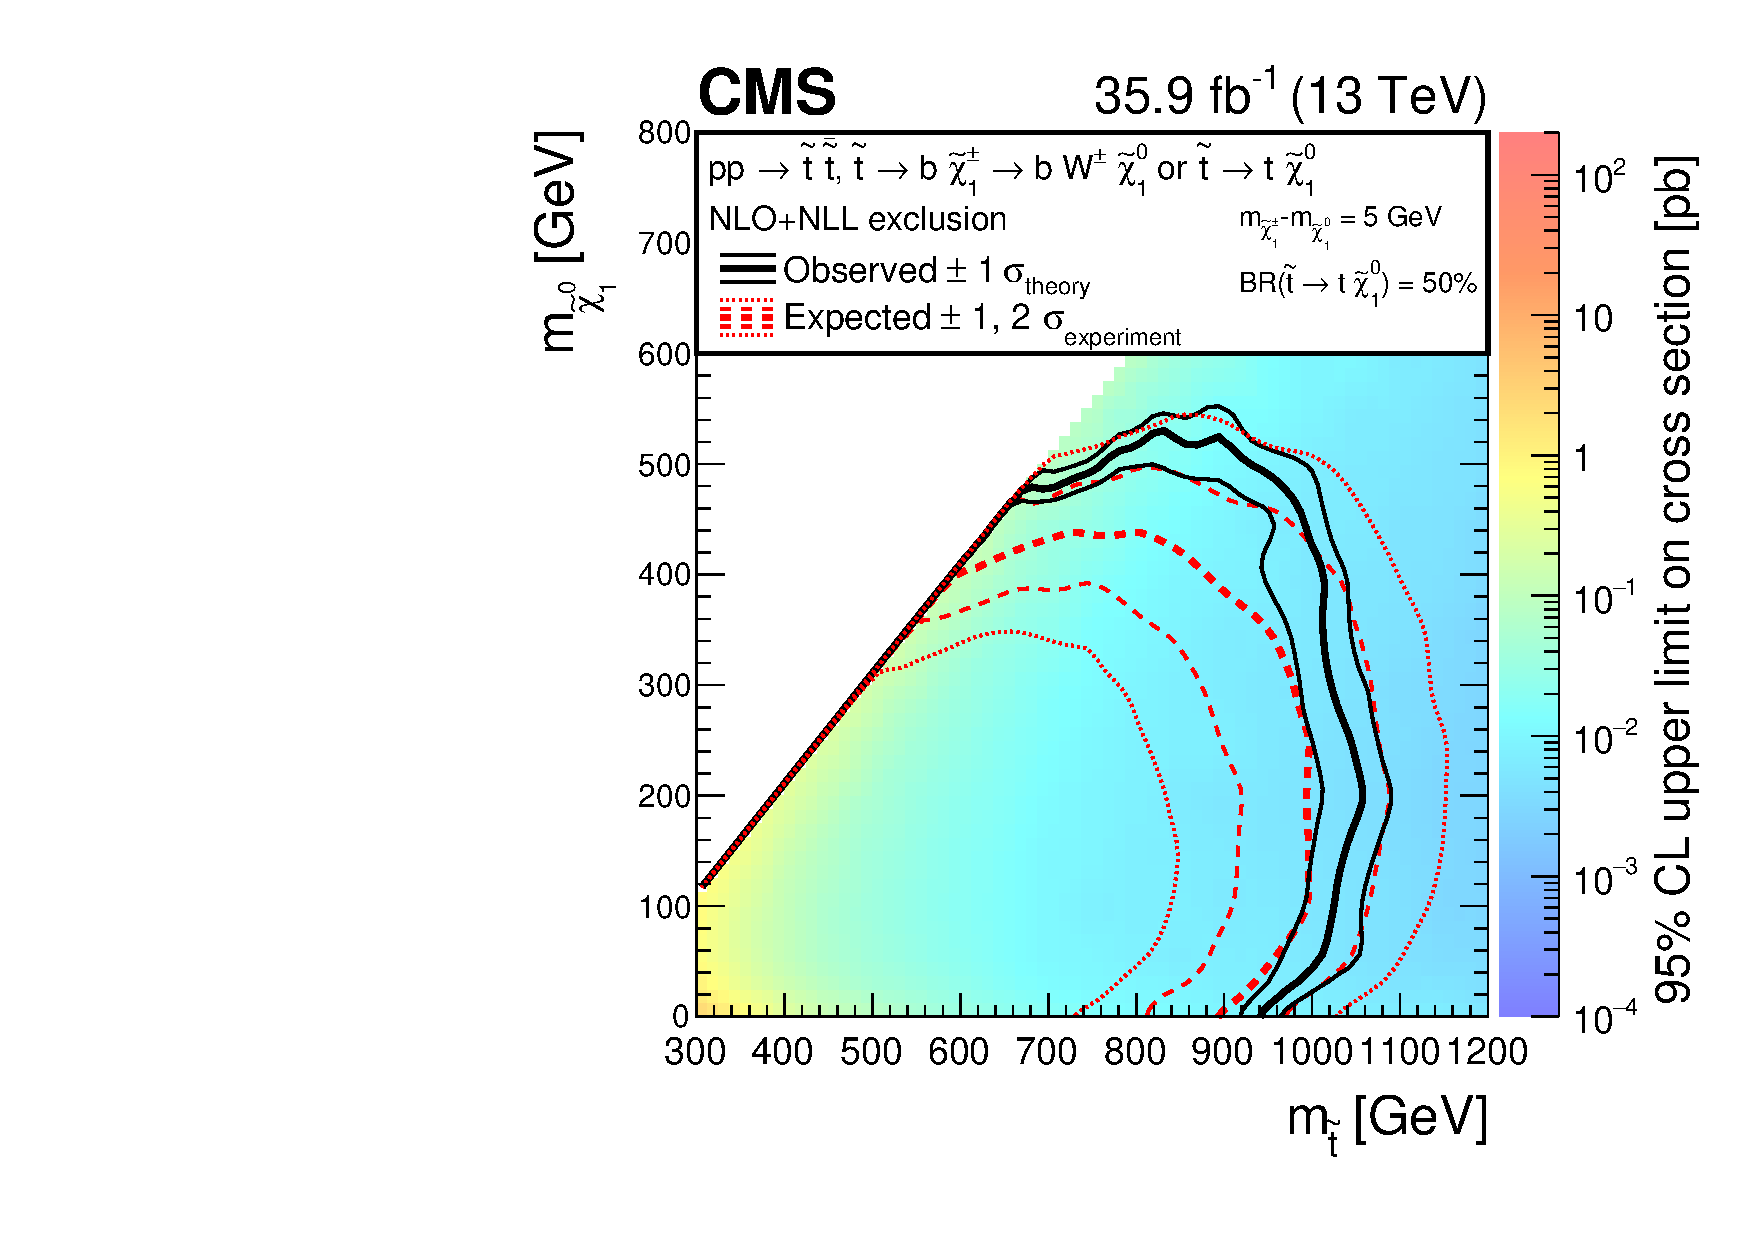
\includegraphics[width=0.45\textwidth]{results/figs/interpretations/T2bt_35p9ifb_Moriond2017_Mar07_XSEC}
	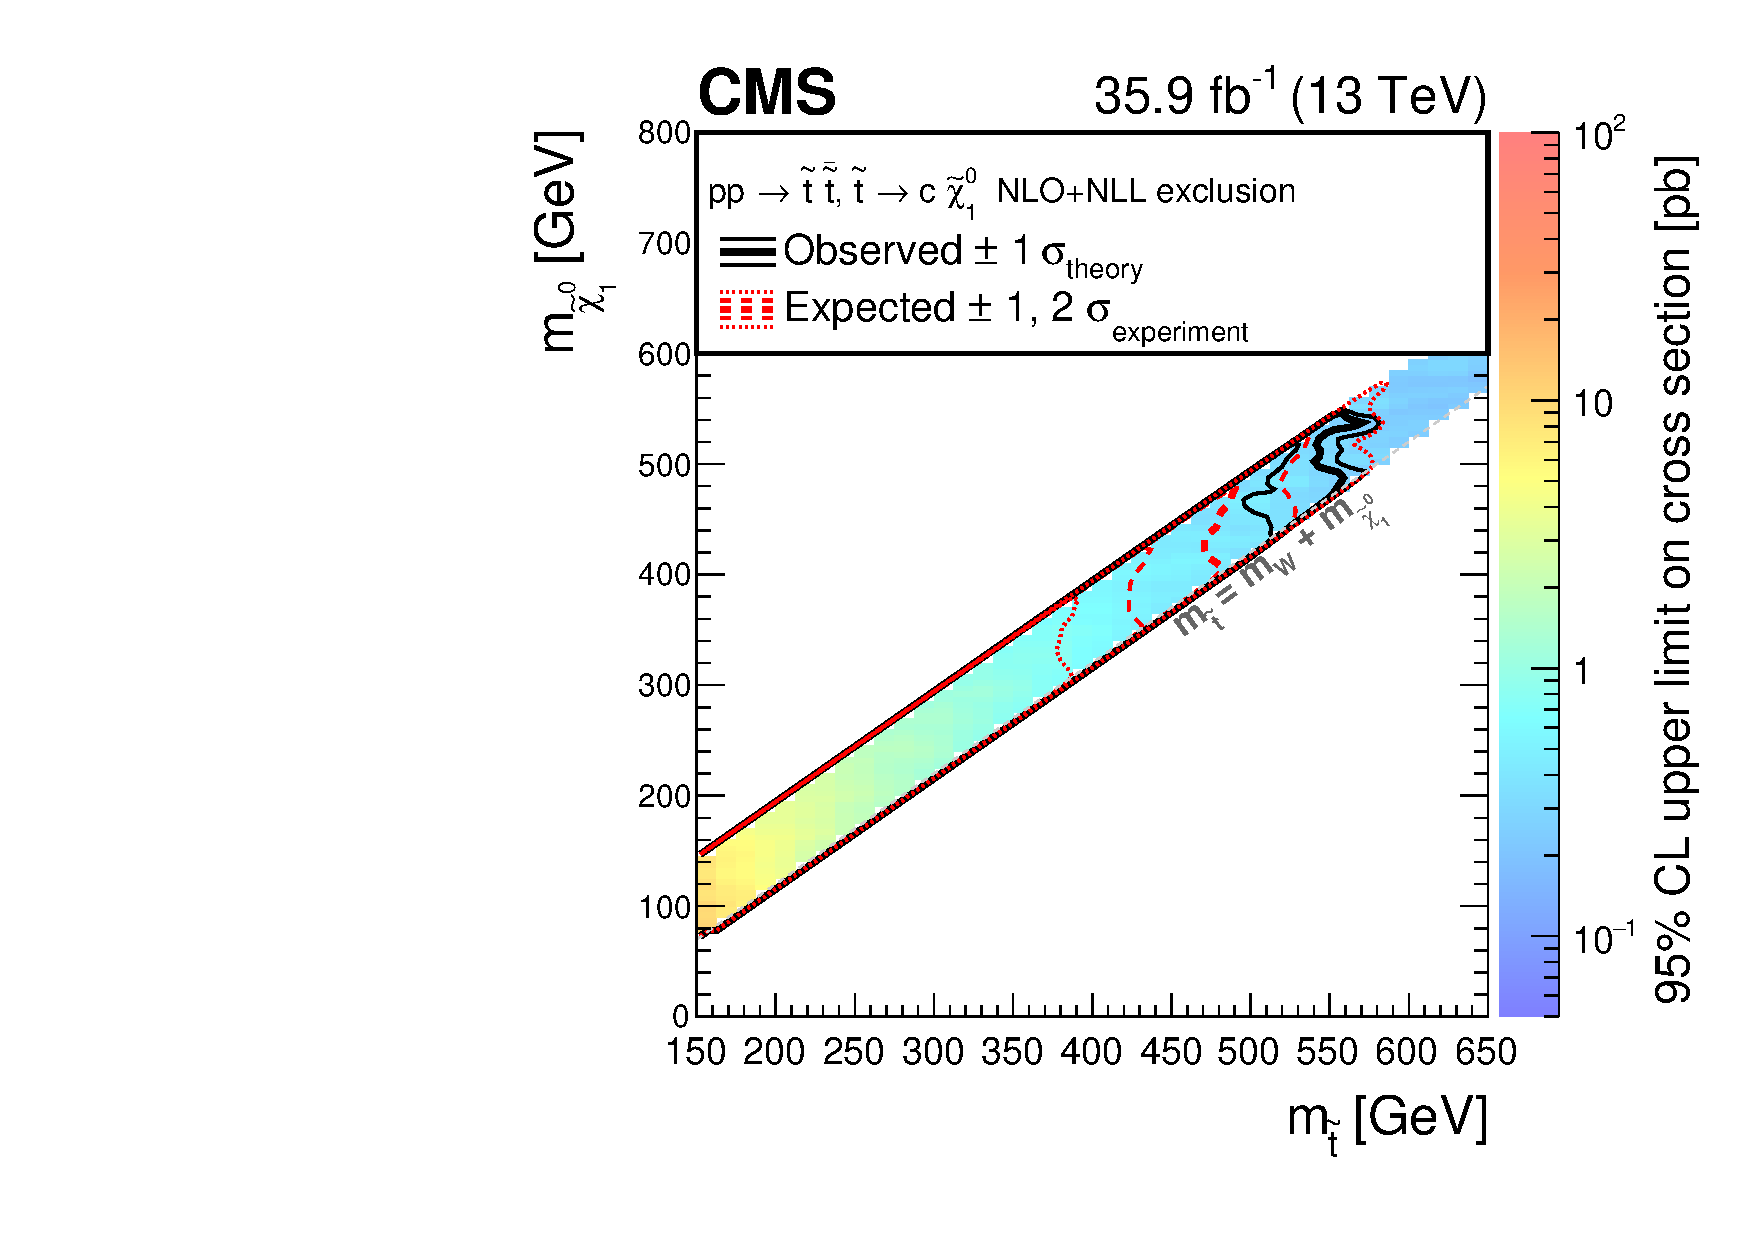
\includegraphics[width=0.45\textwidth]{results/figs/interpretations/T2cc_35p9ifb_Moriond2017_Mar07_XSEC}
	\caption{Exclusion limits at 95\% confidence level for direct top squark production In different decay modes. The top squark may decay through charginos (top left), where the chargino mass is taken as halfway-between the top squark and neutralino; a mixed scenario through charginos and neutralinos (top right), where the chargino mass is fixed to 5\GeV above the neutralino mass; or a compressed scenario, where the top squark is kinematically constrained to decay to charm quarks (bottom). The dashed red lines indicate the expected sensitivity and associated uncertainty, while the black lines indicate the observed exclusion limit and its associated theoretical uncertainty based on the signal cross-section.}
	\label{fig:limitsStop}
\end{figure}

\begin{table}
	\centering
	\begin{tabular}{lrr}
\hline
Simplified & Limit on produced sparticle & Highest limit on the \\
model & mass [GeV] for $m_{\lsp}=$~0\GeV & \lsp mass [GeV] \\
% & (\GeV) & (\GeV)  \\
\hline\hline
Direct squark production: & & \\
Bottom squark & 1175 & 590 \\
Top squark & 1070 & 550 \\
Single light squark & 1050 & 475 \\
Eight degenerate light squarks & 1550 & 775 \\
\hline
Gluino-mediated production: & & \\
$\tilde{g}\rightarrow \bbbar\lsp$ & 2025 & 1400 \\
$\tilde{g}\rightarrow \ttbar\lsp$ & 1900 & 1010 \\
$\tilde{g}\rightarrow q\bar{q}\lsp$ & 1860 & 1100 \\
\hline
\end{tabular}
	\caption{Summary of 95\% CL exclusion limits on the masses of SUSY particles (sparticles) produced by various simplified models. The limit on the produced sparticle is listed for a massless \lsp, along with the greatest excluded mass of \lsp for any mass of produced sparticle.}
	\label{tbl:limits}
\end{table}

% --------------------------------------------------------------------------- %
% --------------------------------------------------------------------------- %


This chapter makes use of figures and tables from the \mttwo paper and internal analysis note to illustrate the analysis design, methodology, and results. This work was made possible by contributions from the rest of the Surf \& Turf group, our collaborators at ETH Zurich, and the many other CMS members in the SUSY group and beyond.

% --------------------------------------------------------------------------- %
% --------------------------------------------------------------------------- %

% --------------------------------------------------------------------------- %
% --------------------------------------------------------------------------- %
\chapter{Extending the All-Hadronic Search}
\label{ch:soft}

The results presented in this analysis thus far exclude significant amounts of SUSY parameter phase space compared to previous searches for similar signatures. However, the spectrum of SUSY models that might be realized in nature is wide and varied. As the LHC continues to deliver an increasing amount of collision data, the ability to probe increasing rare and more subtle signatures increases. 

In this final section we discuss extensions to the \mttwo analysis that modify the search to target additional SUSY models, in particular those which may produces very low-\pt leptons in the final state, otherwise known as {\it soft leptons}. By requiring a lepton in the final state, the previously irreducible invisible Z background of the all-hadronic analysis is greatly suppressed, and in principle one might hope to probe additional phase space for new physics.

\section{Natural Supersymmetry and EWKinos}
\label{sec:natural}

There are a multitude of supersymmetric models which solve some of the theoretical issues of the SM, namely the hierarchy problem discussed in section \ref{sec:smIssues}. However, given the vast parameter of SUSY phase space which might satisfy physical constraints, it is sometimes considered theoretically unfavorable for a particular model to accomodate physical phenomena at the expense of a theoretical explanation, instead relying on the ``fine-tuning'' of physical parameters to remain consistent with observations in nature. The property of a theoretical model that consistently explain observed phenomena with minimal tuning is often referred to as its {\it naturalness}, and can be quantified as a the likeliness for measured observables to be contained in some subset of the total parameter space such that the model satisfies experimental constraints.

A SUSY model that solves some of the fine-tuning problems present in the SM without introducing additional fine-tuning problems of its own is an example of {\it natural supersymmetry}, and is theoretically appealing as an elegant solution to the would-be fine-tuning issues in the SM \cite{Casas:2014eca}. Such natural models often share similar characteristics, including a relative mixing of the supersymmetric partners of the Higgs and electroweak gauge bosons (EWKinos) into mass eigenstates with a highly-degenerate spectrum. Charged EWKinos (\chipm) can decay into neutral EWKinos or the lightest supersymmetric particle (\chiz) in cascades with leptons in the final state. In compressed mass spectra where the mass difference between the charged and neutral EWKinos is small, the outgoing leptons will be soft, and searches targeting soft leptons in the final state can be a useful tool in searches for natural SUSY.

\section{The Soft Lepton Search}
\label{sec:softlep}

A preliminary search extending the all-hadronic analysis was conducted on 2.3\fbinv of data collected by the CMS detector through 2015 \cite{CMS-PAS-SUS-16-011}. The results of this preliminary analysis are presented here and interpreted in the context of two simplified SUSY models with compressed mass spectra.

\subsection{Event Selection}
\label{subsec:softevents}
The soft lepton search defines a baseline selection similar to that used in the \mttwo analysis, with the notable exception of requiring a soft electron (muon) with $5 < \pt < 20\GeV$ in the barrel region, $|\eta| <$ 1.4442 (1.479). Similar \MET triggers are used, with a minimum \MET requirement of 200\GeV to saturate the trigger efficiency. Identical \dphilong and \htovermet requirements are used to protect against \MET mismeasurements, and
to reject dilepton events the same lepton vetoes are applied to additional leptons in the event. There is an additional requirement on transverse mass of the soft leptons such that $\mt > 20\GeV$, in order to reduce the background contribution from $Z\rightarrow\tau\tau$ events. Events must contain at least 1 jet and a minimum of $\HT > 200\GeV$ of hadronic activity.

Following the baseline selection above, events are further categorized into topological regions using the \HT, \MET, and \nj content, as well as the number of b-tags \nbsoft and \nbhard, where a b-jet is considered soft if $20 < \pt < 50\GeV$, and hard if $\pt > 50\GeV$. There are three ``tail'' regions corresponding to different kinematic variables:
\begin{itemize}
	\item \nb (soft or hard) $\geq 3$
	\item $\MET > 500\GeV$ and $\nb \leq 3$
	\item $\HT > 1000\GeV$, $\nb \leq 3$, and $\MET < 500\GeV$
\end{itemize}
The remaining phase space is divided into topological regions as follows:
\begin{itemize}
	\item \MET : [200,300], [300,500] \GeV. These are merged in the monojet regions with b-tags.
	\item \nb : There are four \nb regions, \nb = 0, \nbsoft = [1,2] (with \nbhard = 0), and \nbhard = [1,2], respectively referred to as the 0b, soft b, and hard b regions.
	\item \nj : In regions with no b-tags, events are binned in regions with 1, 2-3, 4-5, or $\geq$6 jets. In regions with one or more b-tags, events are binned in regions with 1, 2-3, or $\geq$4 jets.
\end{itemize}
Finally, each topological region is subdivided into three bins of \mt: [20,90], [90,120], and $\geq$120\GeV. In total, there are 21 topological regions each subdivided into 3 \mt bins.

\subsection{Backgrounds}
\label{subsec:softbkgs}
The background for the soft lepton analysis can be categorized into three separate sources:
\begin{itemize}
	\item {\it Single Lepton}: real SM processes can generate events with a single lepton in the final state. Typically such events contain a single leptonically decaying W boson (from either W production, top quark production, or other rare processes), and also generate significant missing energy due to the neutrino associated with the W decay.
	\item {\it Dilepton}: SM events with two (or more) leptons in the final state can be mischategorized when other leptons are misidentified or not reconstructed. Typically such events are due to two leptonically decaying W bosons (from either \ttbar or diboson production), where one of the W-associated leptons is not found. Because there are usually two neutrinos contributing to the \MET vector, \mt is less effective in discriminating against this background.
	\item {\it Fake Lepton}: events without any lepton in the final state (such as QCD multijet production of \znunu) can enter the signal region if a jet is misidentified as a lepton or a non-prompt lepton passes the lepton selection. This background is highly suppressed and typically negligible in all but some high-\mt regions.
\end{itemize}

%single lepton estimate
\subsection{Single Lepton Estimate}
\label{subsec:soft1Lestimate}
The single lepton background is primarily due to highly-asymmetric W decays where the neutrino carries a large fraction of the W momentum, resulting in a large \MET and a soft lepton. These events are greatly suppressed by sampling the \mt distribution as values greater than the W mass, and is estimated in all signal regions using a control region with an inverted asymmetry. A single high-\pt control region is created by selecting events with a single lepton above the corresponding \MET threshold in a given signal region (\pt $\geq$ 200, 300, or 500 \GeV), with an maximum threshold on the missing energy $\MET <60\GeV$ so that the W momentum distribution is kinematically similar to that in the signal regions. The number of control region events in a given topological region ($N^{\text{CR1L}}$) is multiplied by the ratio of SR-to-CR events as calculated in simulation ($R_{\text{MC}}^{\text{SR/CR1L}}$) for the region, and extrapolated into bins of \mt based on simulation ($k_{\text{MC}}(\mt)$) as described in equation \ref{eq:soft1Lestimate}. The extrapolation in bins of \mt is necessary not only to preserve statistics but because the shape of the \mt distribution in each control region is very different from the signal region distribution, due to the low-\MET requirement in the control region where resolution effects cause a significant smearing in the \mt shape.
\begin{equation}
	N_{1l}^{\text{SR}} = N^{\text{CR1L}} \cdot R_{\text{MC}}^{\text{SR/CR1L}} \cdot k_{\text{MC}}(\mt)
	\label{eq:soft1Lestimate}
\end{equation}

The uncertainties associated with the single lepton estimate account for statistical fluctuations in data and simulation, as well as possible sources of systematic error in simulation propagated to the quantities measured in MC. The polarization modeling is studied in an inclusive W sample and found to be well modeled by simulation, and additional studies reweighting simulation based on W polarization result in an uncertainty of 10-20\% on the transfer factor $R_{\text{MC}}^{\text{SR/CR1L}}$. Additional uncertainties due to the relative fraction of top and W events, renormalization and factorization scales, lepton efficiency, b-tagging efficiency, jet energy corrections, and uncertainty on top momentum are propagated through simulation, with varying effects between 1-10\%. In addition, multiple uncertainties associated with \mt modeling in simulation are studied, with effects due to W-top fraction and \MET resolution yielding uncertainties ranging between 5-30\% in \mt shape, depending on the relative fraction of top events in a given bin.

%dilepton estimate
\subsection{Dilepton Estimate}
\label{subsec:soft2Lestimate}
Backgrounds due to dilepton events where one lepton is not found are estimated using a control region instead requiring two leptons, replacing the second-lepton veto with a tight requirement for a second, high-\pt lepton. To suppress the contribution from events with fake leptons, the second lepton is required to have a minimum \pt of at least 25\GeV, and the expected statistics, kinematics, and composition of the control region is similar to that of the signal region. Because of the low rate of this background in the signal region (and corresponding low statistics in each control region), the estimate is performed in a similar manner to the single lepton estimate, but with an additional extrapolation in the \MET dimension based on simulation. The number of control region events in a given region of \HT, \nj, and \nb ($N^{\text{CR2L}}$) is multiplied by the ratio of SR-to-CR events as calculated in simulation ($R_{\text{MC}}^{\text{SR/CR2L}}$) for that region, and extrapolated into bins of \MET and \mt based on simulation ($k_{\text{MC}}(\MET, \mt)$) as described in equation \ref{eq:soft2Lestimate}. 
\begin{equation}
	N_{2l}^{\text{SR}} = N^{\text{CR2L}} \cdot R_{\text{MC}}^{\text{SR/CR1L}} \cdot k_{\text{MC}}(\MET, \mt)
	\label{eq:soft2Lestimate}
\end{equation}

In addition to statistical fluctuations, the uncertainties associated with the dilepton estimate account for several effects, including lepton acceptance in simulation. Varying the renormalization and factorization scales, lepton efficiency, and jet energy corrections in simulation is propagated to the ratio $R_{\text{MC}}^{\text{SR/CR1L}}$, yielding uncertainties of 1-10\%, 5\%, and 5-20\% respectively (the b-tagging uncertainty is found to be negligible). Because the \zll yield in the control region is slightly different than that in the corresponding signal regions, an additional uncertainty of 5-10\% is assigned to each region based on the relative fraction of \zll events. Possible systematic effects of the \MET and \mt modeling in simulation are also studied in dilepton \ttbar control regions, yielding uncertainties of 10\% (35\%) in the 300-500\GeV ($\geq$500\GeV) \MET regions and 30\% (50\%) in the medium (high) \mt bins.

%fake lepton estimate
\subsection{Fake Lepton Estimate}
\label{subsec:softfakeestimate}
The fake lepton background has multiple contributions from different SM processes. Missing energy mismeasurement may yield a contribution from QCD multijet events, but this background is strongly suppressed due to sufficiently large \MET requirements in every signal region. Additional contributions from electroweak SM processes with zero or one lepton in the final state but significant \MET can also contribute, when a fake lepton is found in a zero lepton event (such as \znunu) or a real lepton lost and a fake lepton found in a one lepton event (such as W production). In most regions, the fake lepton background is negligible (with respect to uncertainties on the other backgrounds), and so the prediction is taken directly from simulation in the low and medium \mt regions with a 100\% uncertainty on the yield. However, because the fake lepton background is not constrained by $\mt < \m_{\text{W}}$ and falls more slowly than other background distributions in \mt, in the high-\mt regions it is more significant and estimated from data. To calculate the predicted yield, a loose-not-tight (L!T) control region is constructed with identical kinematic requirements to the signal region, except the soft lepton is required to pass the loose lepton identification requirements but fail the tight requirements ($N_{\text{data}}^{\text{L!T}}$). Once the contribution from prompt leptons passing the L!T selection ($N_{\text{prompt}}^{\text{L!T}}$), the yield is weighted by the probability that a fake lepton passing the loose selection also passes the tight selection ($\epsilon_{\text{TL}}$). The probability is measured as a function of lepton \pt in a sample of QCD multijet data enriched in fake leptons, selected using a high-statistics sample of QCD events recorded with pure \HT triggers. The fake lepton estimate in each high-\mt signal region is described by equation \ref{eq:softfakeestimate}.
\begin{equation}
	N_{\text{SR}}^{\text{fakes}} = \sum_{\pt} \left( N_{\text{data}}^{\text{L!T}}(\pt) - N_{\text{prompt}}^{\text{L!T}}(\pt) \right) \times \frac{\epsilon_{\text{TL}}(\pt)}{1-\epsilon_{\text{TL}}(\pt)}
	\label{eq:softfakeestimate}
\end{equation}

Based on studies in simulation, the fake-enriched QCD multijet sample has negligible prompt lepton contamination when requiring $\MET < 50\GeV$ and $\mt < 40\GeV$. The tight-to-loose ratio is $\mathcal{O}(10\%)$, and the expected fake yield in the high-\mt bin is $\mathcal{O}(1)$ events. Thus the estimate is dominated by statistics in the L!T region, ranging between 50-100\%.

\subsection{Results and Interpretations}
\label{subsec:softresults}

The predicted background yields are compared with 2.3\fbinv of data collected by the CMS detector through 2015.  No significant deviations from the expected SM background are observed. As with the all-hadronic analysis, the backgrounds are also estimated using a maximum likelihood fitting procedure with a background-only hypothesis as described in section \ref{sec:yields}. Both the pre-fit and post-fit background predictions compared to data are illustrated in figure \ref{fig:softresults}.
\begin{figure}
	\centering
	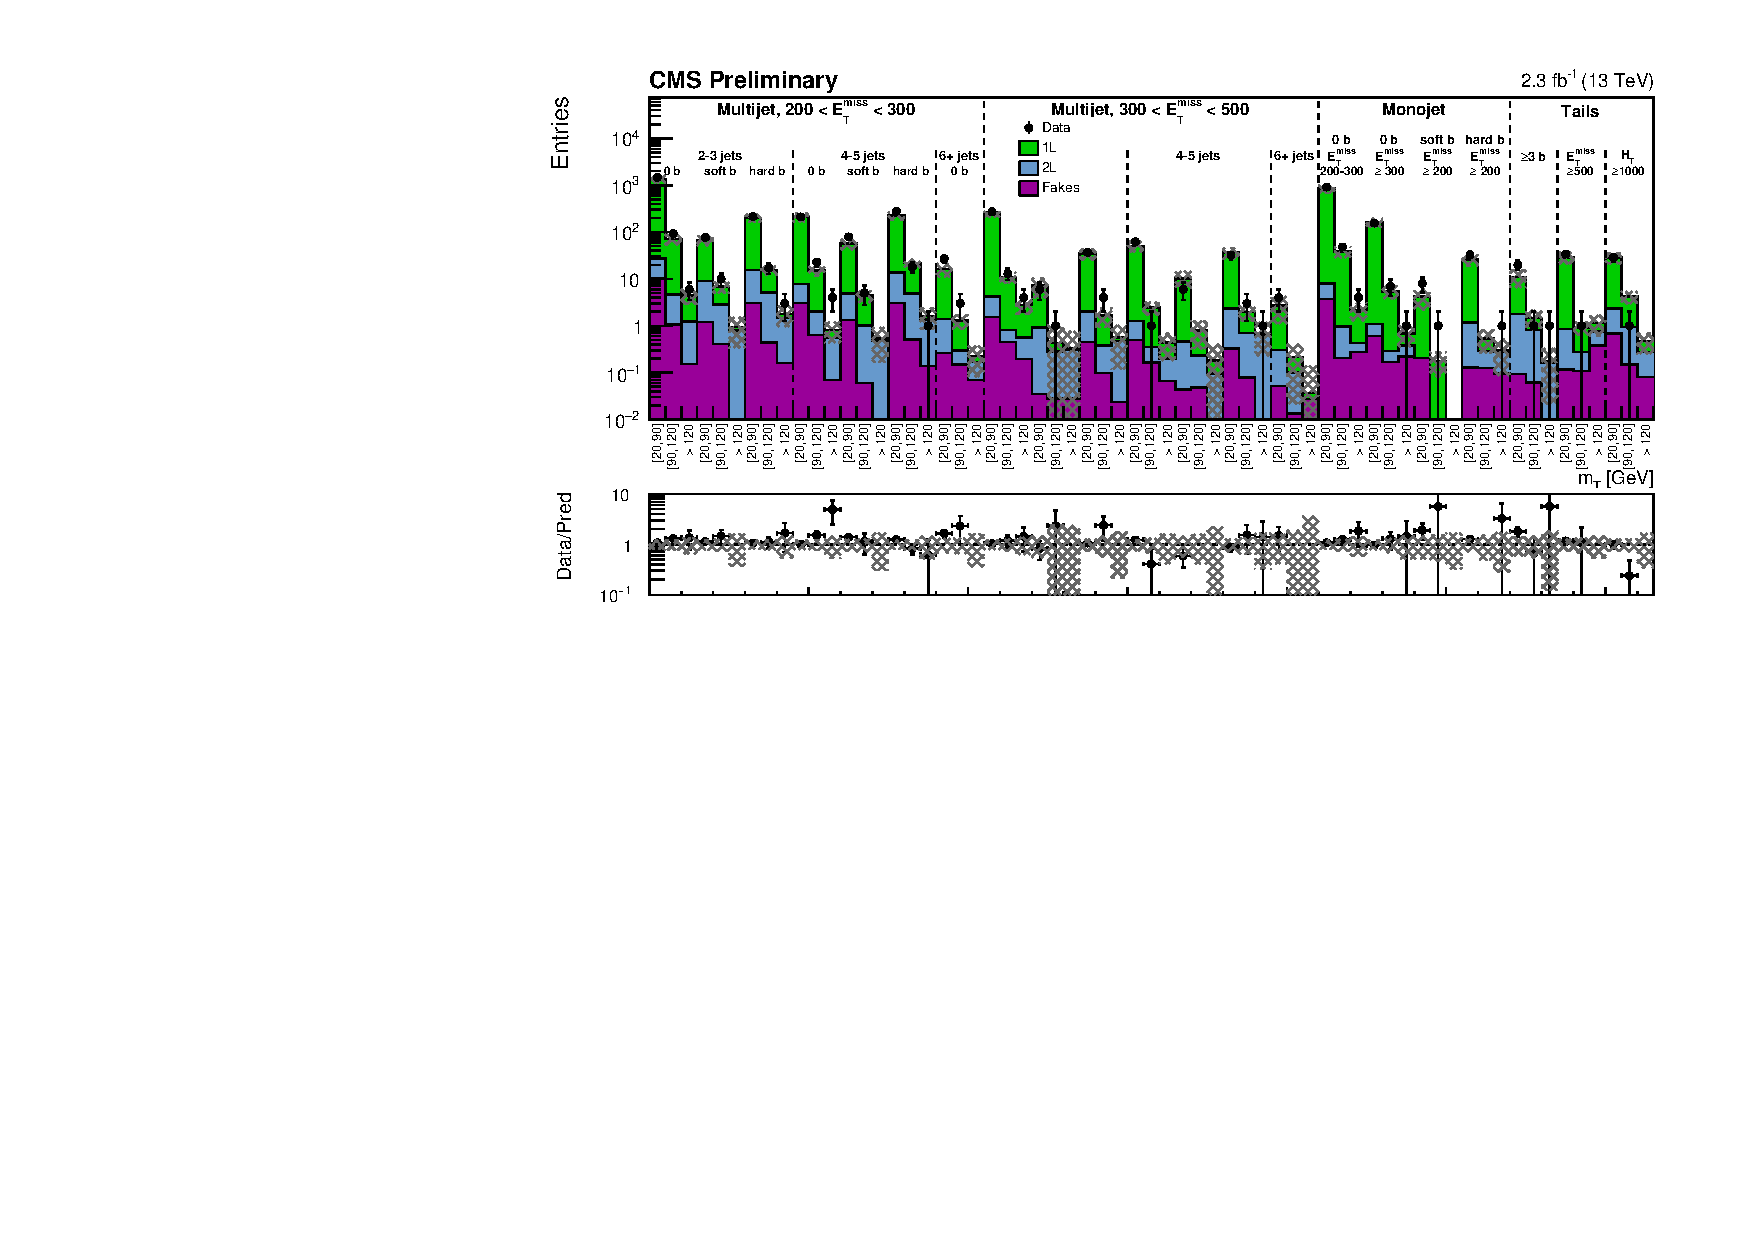
\includegraphics[width=0.95\textwidth]{soft/figs/c_DataVsPrediction_Syst_log}
	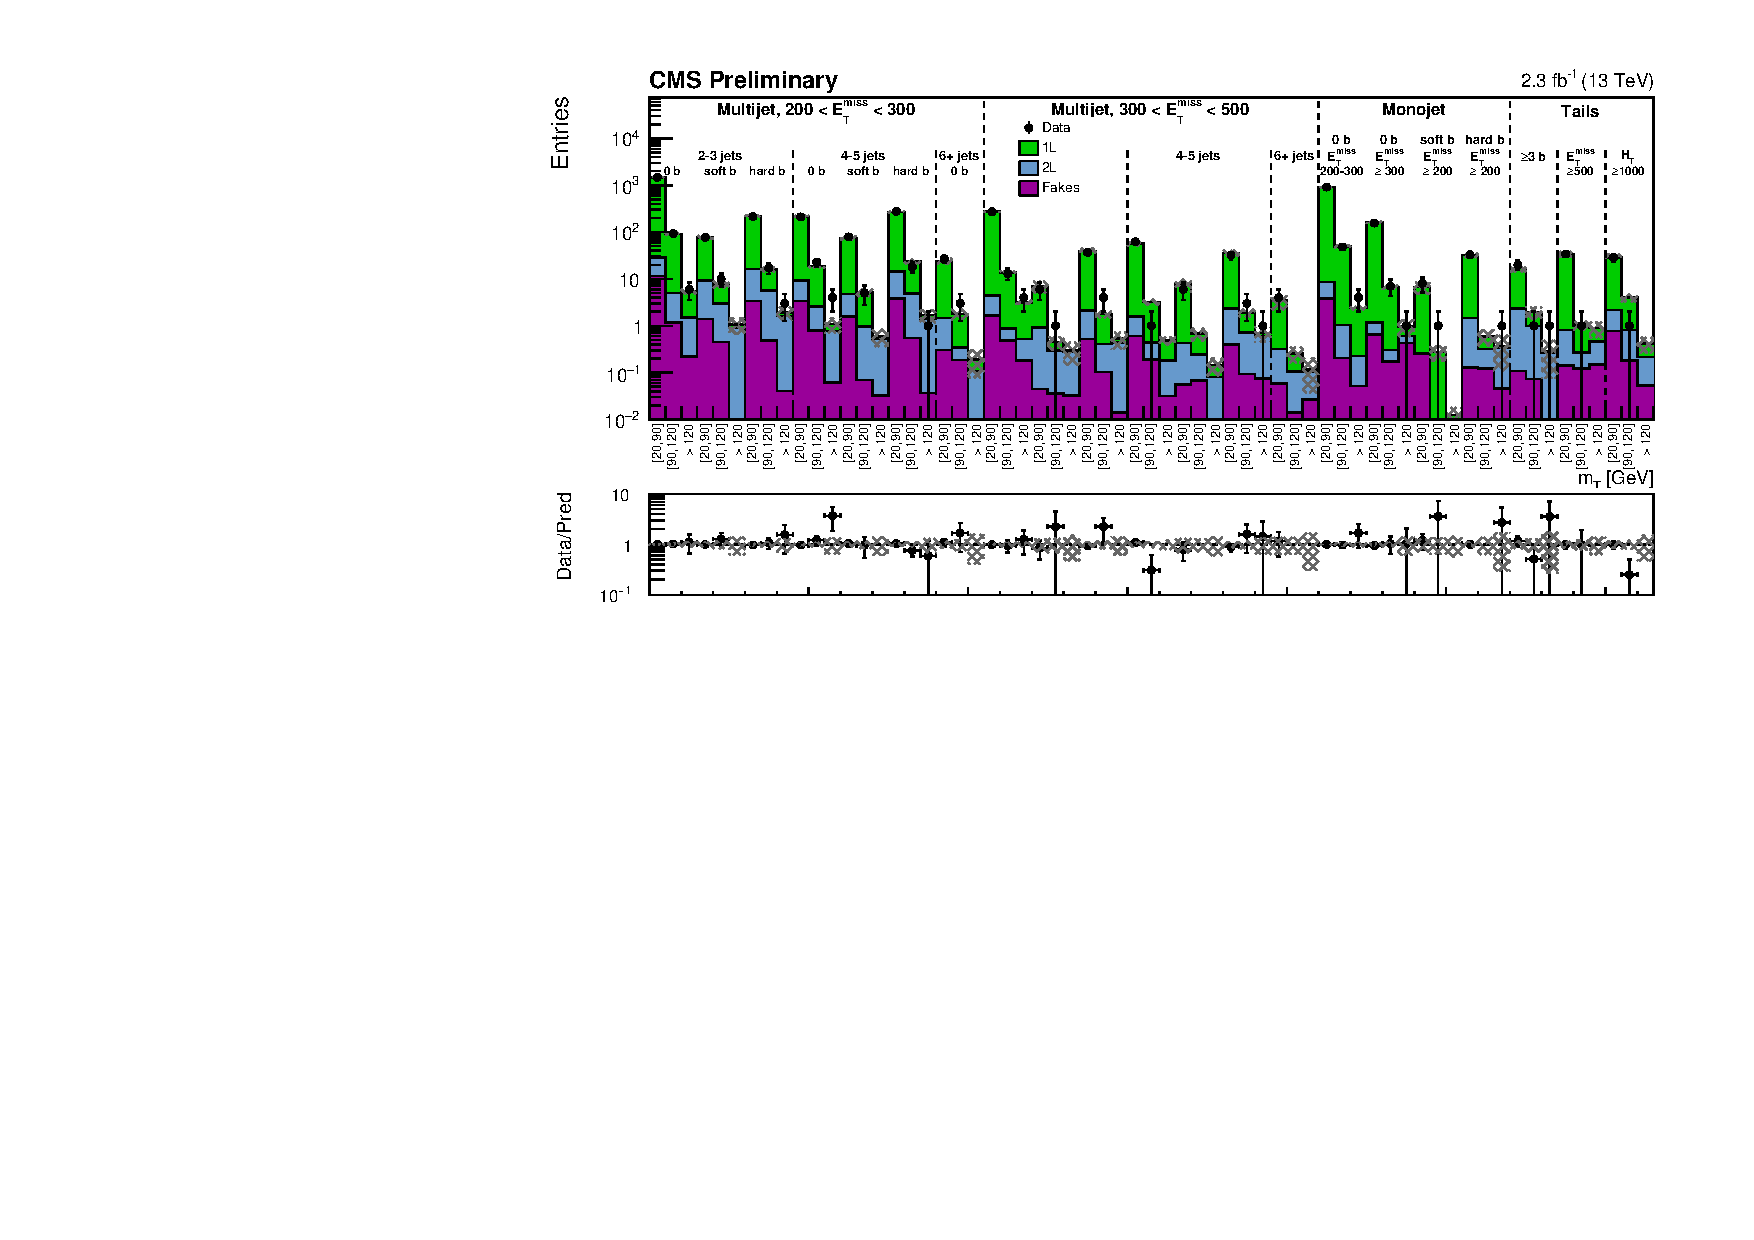
\includegraphics[width=0.95\textwidth]{soft/figs/c_DataVsPostFitEstimates_log}
	\renewcommand{\baselinestretch}{1.0}
	\caption[The predicted background yields compared to the observed number of events in data for pre-fit (top) and post-fit (bottom) background estimates.]{The predicted background yields compared to the observed number of events in data for pre-fit (top) and post-fit (bottom) background estimates. The \mt bins are shown on the $x$-axis, and the grey hatched band represents the total uncertainty on the background yields for the pre-fit background estimates and the fit uncertainty for the post-fit estimates.}
	\label{fig:softresults}
\end{figure}

Additional fits using a background-plus-signal hypothesis are used to set upper limits on the production cross sections of some simplified SUSY models producing soft leptons. A summary of the uncertainties on the simulated signal yield can be found in table \ref{tbl:softsignalSyst}. The post-fit background yield based on these inputs is used to set 95\% confidence level exclusion limits as shown in figure \ref{fig:softlimits}.

\begin{table}
	\centering
	\renewcommand{\baselinestretch}{1.0}
	\caption{Typical values of the systematic uncertainties associated with the simplified SUSY model signal yield for each interpretation in this search.}
	\begin{tabular}{l|c}
\hline
Source & Typical values [\%]  \\
\hline
Integrated luminosity & 2.7  \\
Lepton efficiency & 10  \\
Jet energy scale & 5  \\
b tagging efficiency & 0--20  \\
ISR & 15--30  \\
Renormalization  and factorization scales & 5  \\
Limited size of MC samples & 1--70  \\
\hline
	\end{tabular}
	\label{tbl:softsignalSyst}
\end{table}
\begin{figure}
	\centering
	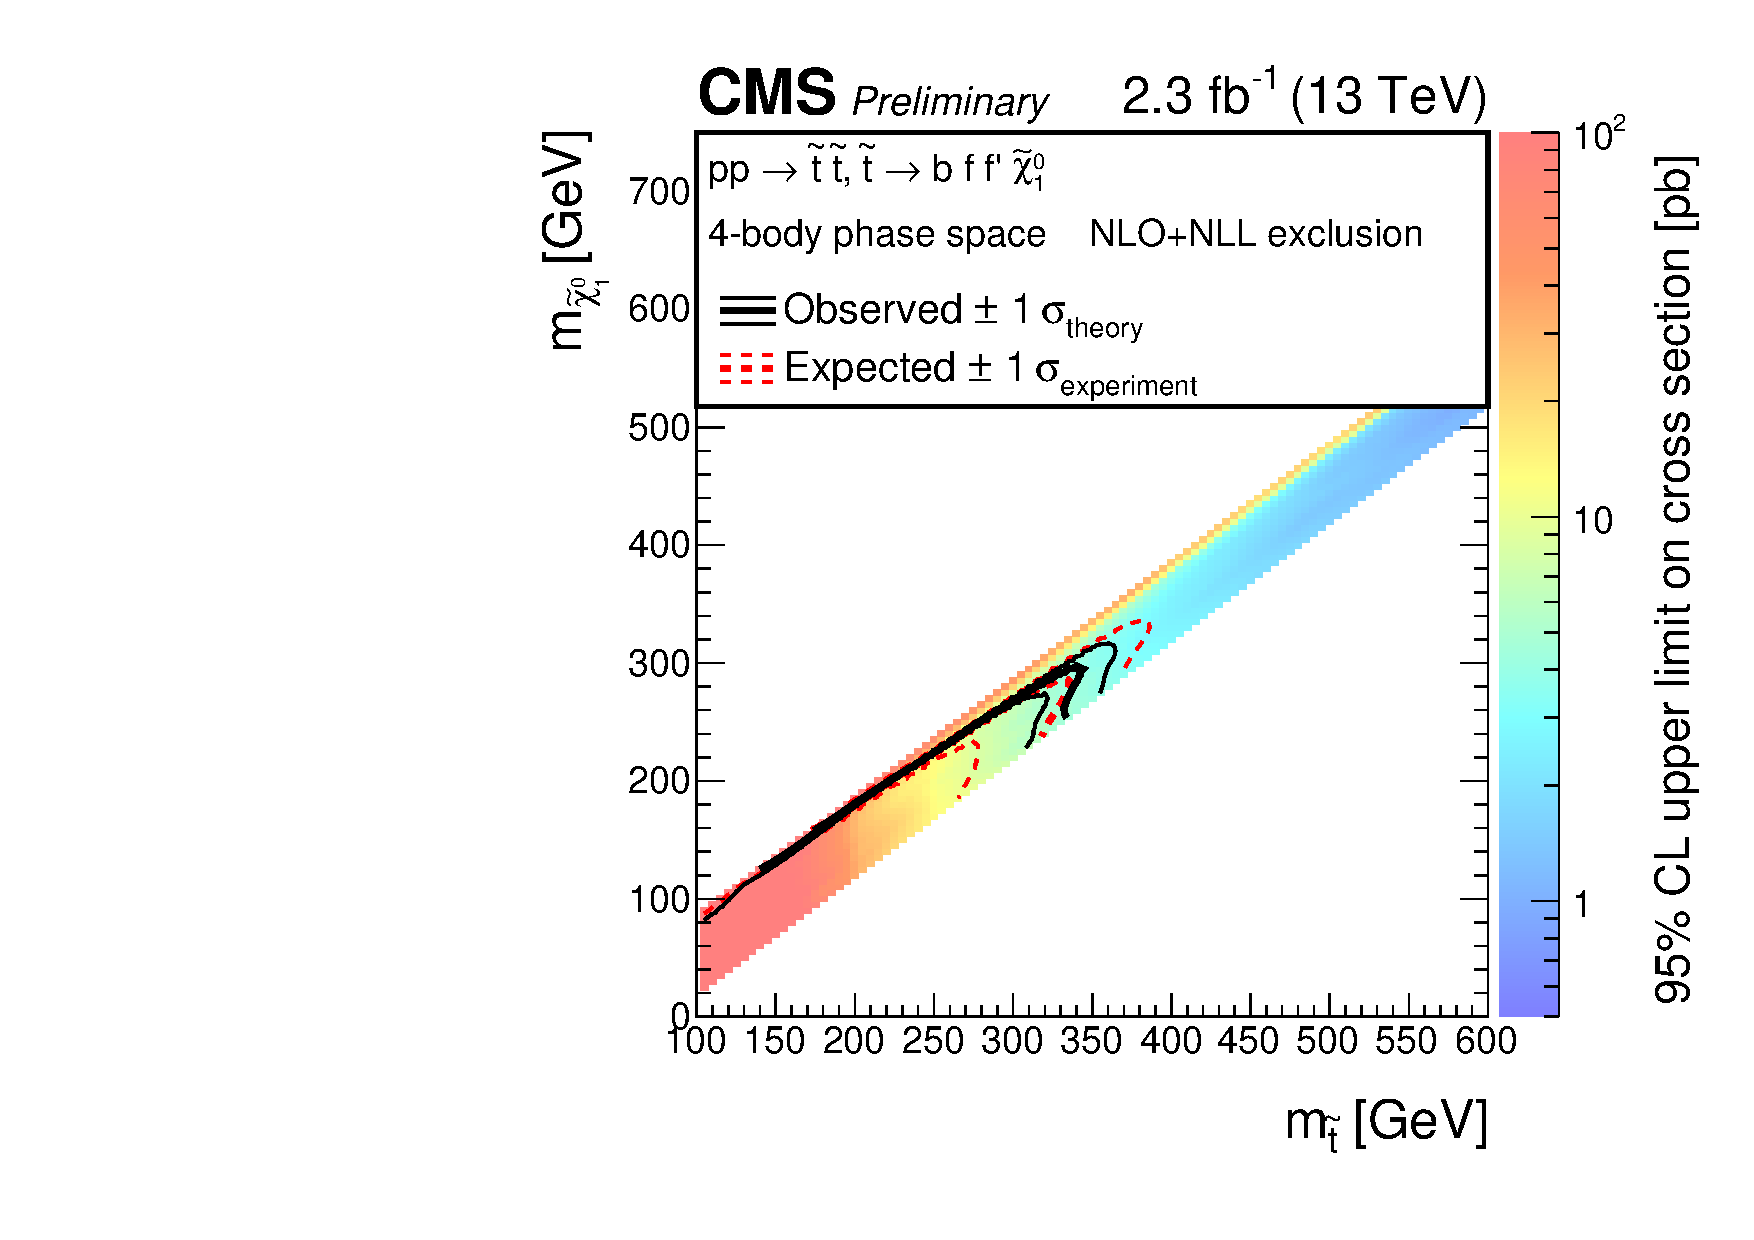
\includegraphics[width=0.48\textwidth]{soft/figs/T2-4bdXSEC}
	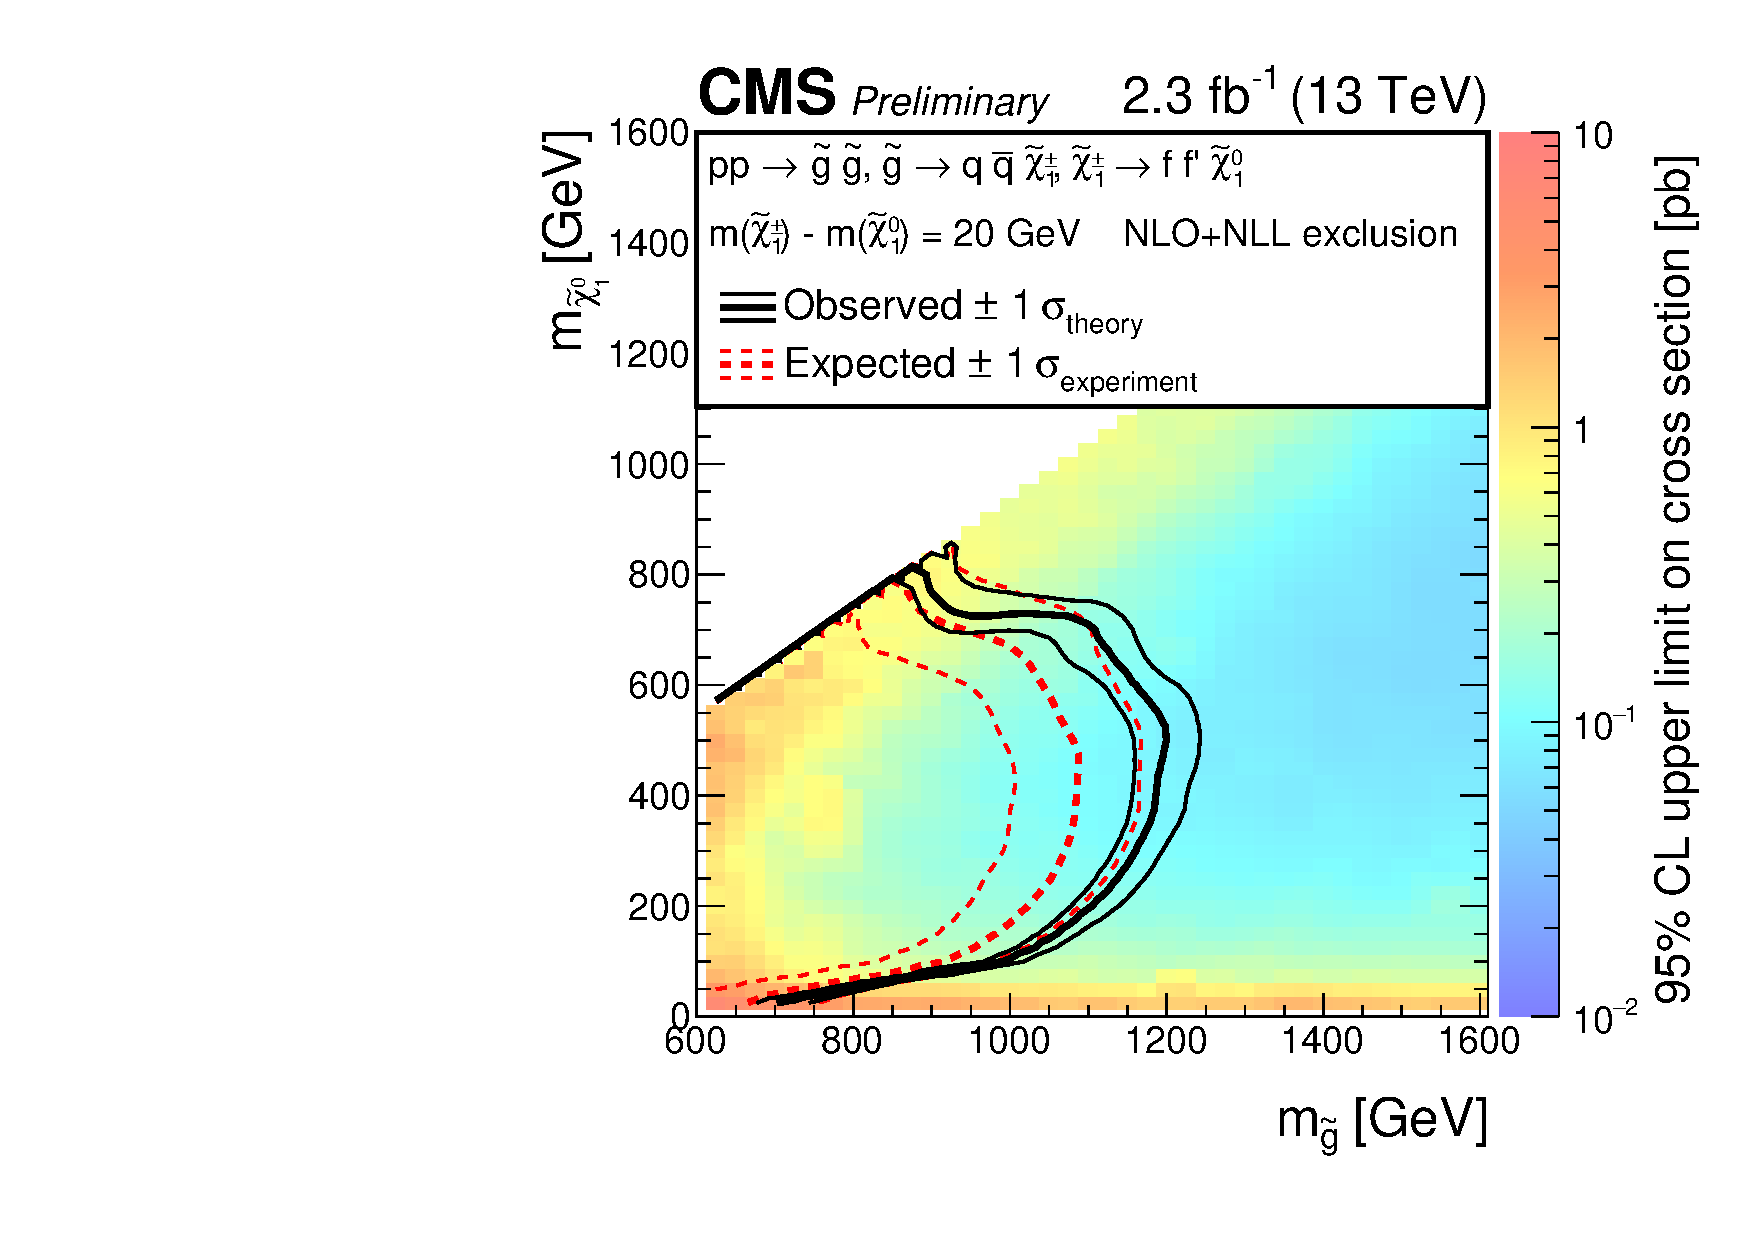
\includegraphics[width=0.48\textwidth]{soft/figs/T5qqqqWWXSEC}
	\renewcommand{\baselinestretch}{1.0}
	\caption[95\% confidence level exclusion limits for top squark (left) and gluino (right) production.]{95\% confidence level exclusion limits for top squark (left) and gluino (right) production. Dashed red lines indicate the expected sensitivity and associated uncertainty, while black lines indicate the observed exclusion limit and its associated theoretical uncertainty based on the signal cross-section.}
	\label{fig:softlimits}
\end{figure}

\section{Future Extensions for an All-Hadronic Search}
\label{sec:future}

The extension of the all-hadronic analysis presented in this section illustrates one possible way to broaden the scope of an all-hadronic search to target additional sectors where new physics might reveal itself. However, there are similar analyses which may supersede the results of a naive single soft lepton search, and an additional question remains -- how much does the extension requiring a soft lepton outperform a traditional all-hadronic analysis? An all-hadronic search should have some discriminating power even against models which always generate soft leptons in the final state (since these leptons will occasionally be lost or mis-identified), and ironically may even have greatly discriminatory power than a soft lepton search when the leptons generated are ultra-soft (\pt $<<5\GeV$) and not reconstructed at all.

To benchmark the possible performance of an improved soft lepton analysis against an all-hadronic search, the performance of the \mttwo analysis on a squark production model generating soft leptons (T5qqWW) is compared to a soft lepton extension. With additional optimization of signal region binning --- in particular a finer binning in the low-\MET regime to target compressed spectra --- and assuming a typical background estimate uncertainty commensurate with previous analyses, it is possible for a soft lepton analysis to outperform an all-hadronic search as illustrated in figure \ref{fig:softfuture}. 
\begin{figure}
	\centering
	\includegraphics[width=0.95\textwidth]{soft/figs/expectedSoftLimit.pdf}
	\renewcommand{\baselinestretch}{1.0}
	\caption[The expected limits of the all-hadronic \mttwo analysis compared with a hypothetical soft lepton extension.]{The expected limits of the all-hadronic \mttwo analysis compared with a hypothetical soft lepton extension. The ``T2qq'' model is a typical squark production model as previously shown in figure \ref{fig:limitsSquark}, whereas the ``T5qqWW'' model is a similar squark production model where the squarks decay in a cascade including charginos, which radiate W bosons that may decay to soft leptons. While the performance of the \mttwo analysis in the hadronic model (green) is similar to the soft lepton model (blue), a soft lepton search can out-perform the all-hadronic equivalent near the diagonal where the mass splitting between the squarks and lightest supersymmetric particle is very small.}
	\label{fig:softfuture}
\end{figure}

Near the mass-diagonal where the parent particle mass (in this case, the squark) is very close to the LSP mass, the soft-lepton search can significantly outperform an all-hadronic equivalent, at the cost of performance in the light-LSP regime. The evidence suggests that a soft-lepton search could be used in conjunction with typical all-hadronic analyses to increase the total excluded phase space when targeting compressed models with nearly-degenerate mass splittings.

This chapter makes use of figures and tables from the soft lepton physics analysis summary to illustrate the analysis design, methodology, and results. This work was made possible by contributions from Giovanni Zevi Della Porta, the rest of the Surf \& Turf group, our collaborators at ETH Zurich, and the many other CMS members in the SUSY group and beyond.

% --------------------------------------------------------------------------- %
% --------------------------------------------------------------------------- %


%% \bibliographystyle{lucas.bst}
\bibliographystyle{plain.bst}
%% \justify
\bibliography{include/refs}

\appendix

\end{document}
